%% =============================================================================
%% main.tex
%% Master Document for Harmonia HIE ArchiMate 3.2 Architecture Specification
%% =============================================================================

\documentclass[10pt,a4paper,oneside]{report}

% Include Custom Styling Packages
\usepackage{styles/harmonia-doc}
\usepackage{styles/harmonia-archimate}

\title{
    \vspace{-2.0cm}
    {\Huge\bfseries\color{harmoniablue} Harmonia}\\[0.4cm]
    {\LARGE\bfseries Health Information Exchange Platform}\\[0.8cm]
    {\large\scshape ArchiMate 3.2 Technical Architecture Specification \& System Reference}
}
\author{
    \textbf{Harmonia Platform Architecture Team}\\
    \texttt{architecture@harmonia.health}
}
\date{September 2026 --- Version 1.0.0}

\begin{document}

% --- Title Page ---
\maketitle
\thispagestyle{empty}

% --- Front Matter ---
\pagenumbering{roman}

%% =============================================================================
%% chapters/00-frontmatter.tex
%% Executive Summary, ArchiMate Foundation & System Terminology
%% =============================================================================

\chapter*{Executive Summary}
\addcontentsline{toc}{chapter}{Executive Summary}

\section*{The Harmonia Platform Overview}

The \textbf{Harmonia Health Information Exchange (HIE)} is a modular, high-availability, distributed healthcare integration platform engineered for HL7 FHIR Release 5 (R5) compliance, real-time HL7 v2 clinical data ingestion, sub-millisecond in-memory cached access, and resilient, audit-compliant workflow execution.

Modern healthcare ecosystems demand zero-loss event streaming, high-throughput message translation, resilient task state persistence, and fine-grained clinical data access across disparate clinical systems. Harmonia addresses these challenges through a cohesive five-tier architectural design and cross-cutting governance framework:
\begin{itemize}
    \item \textbf{Tier 1 --- Presentation Services (\textit{Iris})}: Decoupled Vue 3 / TypeScript single-page applications (\texttt{iris-clinical}, \texttt{iris-console}, \texttt{iris-administration}) supported by a dual-port Jakarta EE Backend-For-Frontend (BEFE) gateway separating clinical read interfaces from administrative operational controls.
    \item \textbf{Tier 2 --- Interface \& Gateway Services (\textit{Pylai})}: High-throughput bidirectional MLLP and REST ingress and egress dispatch gateways, featuring dedicated destination-isolated queues to eliminate head-of-line blocking across external hospital systems (PAS, EMR, LIS, RIS-PACS).
    \item \textbf{Tier 3 --- Transport \& Workflow Services (\textit{Petasos} \& \textit{Energeia})}: An active-active Apache ActiveMQ Artemis messaging cluster providing sub-2-second failover and zero message loss, paired with the Ponos/Praxis/Erga modular Apache Camel workflow execution engine operating on canonical task instances (\textit{Pragma}).
    \item \textbf{Tier 4 --- Distributed Cache Services (\textit{Hestia Mneme})}: An in-memory Infinispan 15+ distributed cache grid delivering sub-millisecond retrieval of active clinical tasks, transaction states, and resource models with asynchronous write-behind persistence.
    \item \textbf{Tier 5 --- Persistence Services (\textit{Hestia Mnemosyne})}: Durable long-term relational persistence uniting PostgreSQL 16+ database engines with Spring Boot HAPI FHIR JPA and Operations JPA servers.
    \item \textbf{Cross-Cutting Governance \& Security (\textit{Themis} \& \textit{Calliope})}: Zero-trust role- and attribute-based access control (RBAC/ABAC), dual-gate Protected Health Information (PHI) audit logging, and centralized canonical domain data schemas (DTOs).
\end{itemize}

\section*{Structure and Scope of the Reference Publication}

This document serves as the authoritative Harmonia Architecture, Implementation, and Deployment Reference. To address the diverse requirements of enterprise architects, integration engineers, system administrators, and clinical application developers, the documentation is divided into nine major Parts and twelve comprehensive Appendices:

\begin{itemize}
    \item \textbf{PART I: Foundations (Chapters 1--4)}: Formulates platform motivation, the healthcare integration context, classical conceptual taxonomy, and business/clinical architecture.
    \item \textbf{PART II: Platform Architecture (Chapters 5--12)}: 5-Tier application component architecture, boundary gateways (Pylai), messaging transport (Petasos), collaboration (Agora), workflow orchestration (Energeia), presentation portals (Iris), and FHIR R5 Provider Registry core services.
    \item \textbf{PART III: Information \& Integration (Chapters 13--15)}: Canonical information models, FHIR R5 schemas, HL7 v2 transformations, and MLLP integration guide.
    \item \textbf{PART IV: Middleware Architecture (Chapters 16--20)}: Clustered ActiveMQ Artemis HA, Infinispan distributed caching, PostgreSQL/HAPI FHIR R5 persistence, and Matrix Synapse homeserver architecture.
    \item \textbf{PART V: Runtime Architecture (Chapters 21--26)}: Container packaging, MicroK8s pod scheduling, single-node resilience, physical deployment, Themis security architecture, and governed PHI logging.
    \item \textbf{PART VI: Normal Deployment (Chapters 27--32)}: Declarative configuration hierarchy, properties reference, Ubuntu host preparation, normal MicroK8s deployment runbooks, and undeployment/retention.
    \item \textbf{PART VII: Paradeigma Simulation (Chapters 33--35)}: Synthetic clinical generators, scenario framework, workload deployment runbooks, and strict production isolation guardrails.
    \item \textbf{PART VIII: Development (Chapters 36--38)}: Development environment, architecture invariants, and implementation guides for Ergon activity modules and Praxis workflow sequences.
    \item \textbf{PART IX: Operations (Chapters 39--40)}: Failure operations, recovery guarantees, operational runbooks, and PHI-aware logging implementation guide.
    \item \textbf{APPENDICES (Appendices A--L)}: Authoritative registers and checklists: Appendix A (Glossary), Appendix B (System Inventory), Appendix C (Module Register), Appendix D (Middleware Matrix), Appendix E (Configuration Register), Appendix F (Port/Protocol Register), Appendix G (Image Register), Appendix H (Kubernetes Register), Appendix I (Persistence Register), Appendix J (Dependency Matrix), Appendix K (Normal Deployment Checklist), Appendix L (Paradeigma Deployment Checklist).
\end{itemize}

\section*{ArchiMate 3.2 Architectural Modeling Framework}
\addcontentsline{toc}{section}{ArchiMate 3.2 Architectural Modeling Framework}

To ensure complete structural rigor, unambiguous domain boundaries, and formal traceability across business, application, and infrastructure tiers, this specification is authored strictly in accordance with \textbf{The Open Group ArchiMate 3.2 Standard}.

\begin{figure}[htbp]
    \centering
    \begin{adjustbox}{max width=\textwidth}
        %% =============================================================================
%% diagrams/legend.tex
%% ArchiMate 3.2 Architectural Notation & Relationship Legend
%% =============================================================================
\begin{tikzpicture}[node distance=1.0cm and 0.8cm, auto]

    % --- Background Plate: Layer Color Palette ---
    \draw[archi-plate-bg] (-0.8, 4.0) rectangle (15.8, 6.2);
    \node[archi-plate-title] at (-0.6, 6.0) {ArchiMate 3.2 Layer Color Palette};

    \node[archi-stakeholder, minimum width=2.1cm, minimum height=0.9cm] (l_motiv) at (0.3, 4.9) {\archibadge{Motivation}Motivation};
    \node[archi-capability, minimum width=2.1cm, minimum height=0.9cm] (l_strat) at (2.7, 4.9) {\archibadge{Strategy}Strategy};
    \node[archi-business-service, minimum width=2.1cm, minimum height=0.9cm] (l_biz) at (5.1, 4.9) {\archibadge{Business}Business};
    \node[archi-app-component, minimum width=2.1cm, minimum height=0.9cm] (l_app) at (7.5, 4.9) {\archibadge{Application}Application};
    \node[archi-data-object, minimum width=2.1cm, minimum height=0.9cm] (l_data) at (9.9, 4.9) {\archibadge{Data}Data Object};
    \node[archi-node, minimum width=2.1cm, minimum height=0.9cm] (l_tech) at (12.3, 4.9) {\archibadge{Technology}Technology};
    \node[archi-deployment-node, minimum width=2.1cm, minimum height=0.9cm] (l_phys) at (14.7, 4.9) {\archibadge{Physical}Physical/K8s};

    % --- Background Plate: Relationships ---
    \draw[archi-plate-bg] (-0.8, 0.4) rectangle (15.8, 3.6);
    \node[archi-plate-title] at (-0.6, 3.4) {Standard ArchiMate 3.2 Relationship Connectors};

    % Row 1 of relationships (Structural & Dependency)
    \node[coordinate] (r1_src) at (0.0, 2.3) {};
    \node[coordinate] (r1_dst) at (2.4, 2.3) {};
    \draw[archi-composition] (r1_src) -- node[above=1pt, font=\sffamily\scriptsize\bfseries]{Composition} (r1_dst);

    \node[coordinate] (r2_src) at (4.0, 2.3) {};
    \node[coordinate] (r2_dst) at (6.4, 2.3) {};
    \draw[archi-aggregation] (r2_src) -- node[above=1pt, font=\sffamily\scriptsize\bfseries]{Aggregation} (r2_dst);

    \node[coordinate] (r3_src) at (8.0, 2.3) {};
    \node[coordinate] (r3_dst) at (10.4, 2.3) {};
    \draw[archi-assignment] (r3_src) -- node[above=1pt, font=\sffamily\scriptsize\bfseries]{Assignment} (r3_dst);

    \node[coordinate] (r4_src) at (12.0, 2.3) {};
    \node[coordinate] (r4_dst) at (14.4, 2.3) {};
    \draw[archi-realization] (r4_src) -- node[above=1pt, font=\sffamily\scriptsize\bfseries]{Realization} (r4_dst);

    % Row 2 of relationships (Dynamic & Dependency)
    \node[coordinate] (r5_src) at (0.0, 1.1) {};
    \node[coordinate] (r5_dst) at (2.4, 1.1) {};
    \draw[archi-serving] (r5_src) -- node[above=1pt, font=\sffamily\scriptsize\bfseries]{Serving} (r5_dst);

    \node[coordinate] (r6_src) at (4.0, 1.1) {};
    \node[coordinate] (r6_dst) at (6.4, 1.1) {};
    \draw[archi-access] (r6_src) -- node[above=1pt, font=\sffamily\scriptsize\bfseries]{Access} (r6_dst);

    \node[coordinate] (r7_src) at (8.0, 1.1) {};
    \node[coordinate] (r7_dst) at (10.4, 1.1) {};
    \draw[archi-flow] (r7_src) -- node[above=1pt, font=\sffamily\scriptsize\bfseries]{Flow} (r7_dst);

    \node[coordinate] (r8_src) at (12.0, 1.1) {};
    \node[coordinate] (r8_dst) at (14.4, 1.1) {};
    \draw[archi-triggering] (r8_src) -- node[above=1pt, font=\sffamily\scriptsize\bfseries]{Triggering} (r8_dst);

\end{tikzpicture}

    \end{adjustbox}
    \caption{ArchiMate 3.2 Visual Modeling Notation, Layer Color Palette, and Relationship Types}
    \label{fig:archimate_legend}
\end{figure}

\section*{Classical Architectural Nomenclature \& System Meanings}
\addcontentsline{toc}{section}{Classical Architectural Nomenclature \& System Meanings}

Harmonia adopts naming conventions rooted in classical Greek mythology and philosophy. Each name explicitly reflects the functional responsibility and domain boundary of the underlying software component.

\begin{table}[htbp]
\centering
\small
\begin{tabularx}{\textwidth}{l p{3.2cm} p{3.5cm} X}
\toprule
\textbf{Subsystem} & \textbf{Architectural Role} & \textbf{Classical Origin} & \textbf{Platform Responsibilities} \\
\midrule
\textbf{\texttt{Harmonia}} & Health Integration Environment & \textit{Harmonia} --- Goddess of concord and balance. & Overall platform uniting clinical protocols, streaming messaging, cache grids, and relational storage. \\
\addlinespace
\textbf{\texttt{Petasos}} & Messaging Transport Subsystem & \textit{Petasos} --- Winged hat of Hermes, symbol of swift dispatch. & Clustered ActiveMQ Artemis messaging, durable queues, client failover, and \texttt{PetasosMessage} envelopes. \\
\addlinespace
\textbf{\texttt{Energeia}} & Workflow Services & \textit{Energeia} --- Aristotelian actuality and continuous activity. & Top-level workflow services aggregator containing Ponos, Praxis, Erga, and Ponos CLI. \\
\addlinespace
\textbf{\texttt{Ponos}} & WorkEngine Execution Container & \textit{Ponos} --- Personification of industrious toil and labor. & WildFly 31 Jakarta EE 10 WAR container hosting Camel contexts, Petasos conduits, and task worker managers. \\
\addlinespace
\textbf{\texttt{Erga}} & Modular Task Activities & \textit{Erga} --- Plural of \textit{Ergon}, works, deeds, or tasks. & Single-responsibility Camel route components (\texttt{ErgonBase}) executing discrete clinical mappings. \\
\addlinespace
\textbf{\texttt{Praxis}} & Workflow Sequence Orchestrator & \textit{Praxis} --- Structured action or enactment of theory. & Sequence orchestrator chaining ordered Ergon steps and recording multi-phase state checkpoints. \\
\addlinespace
\textbf{\texttt{Pragma}} & Task Instance / State Entity & \textit{Pragma} --- That which has been done, concrete deed. & Canonical task state model holding inputs, outputs, checkpoints, and bidirectional FHIR \texttt{Task} mapping. \\
\addlinespace
\textbf{\texttt{Calliope}} & Canonical Schema Repository & \textit{Calliope} --- Chief Muse of eloquence and harmonious order. & Shared information models, domain DTOs, schemas, and payload envelopes used across all modules. \\
\addlinespace
\textbf{\texttt{Themis}} & Policy Governance Subsystem & \textit{Themis} --- Titaness of divine law and order. & Default-deny ABAC/RBAC authorization engine, PEP interceptors, and non-PHI audit event logging. \\
\addlinespace
\textbf{\texttt{Mneme}} & In-Memory Distributed Cache & \textit{Mneme} --- Muse of active memory and rapid recall. & Infinispan distributed L1 cache grid providing low-latency \texttt{task-cache} and \texttt{tasksequence-cache}. \\
\addlinespace
\textbf{\texttt{Mnemosyne}} & Relational Persistence Tier & \textit{Mnemosyne} --- Titaness of durable memory. & Long-term PostgreSQL storage comprising Spring Boot FHIR JPA and Operations JPA servers. \\
\addlinespace
\textbf{\texttt{Hestia}} & Data Services Subsystem & \textit{Hestia} --- Goddess of the hearth and foundational stability. & Data services aggregator managing caching (Mneme) and persistence (Mnemosyne). \\
\addlinespace
\textbf{\texttt{Iris}} & Presentation Services & \textit{Iris} --- Goddess of the rainbow and divine messenger. & Decoupled multi-portal presentation tier comprising Jakarta EE dual-port BEFE gateway, Clinical UI SPA, Console UI SPA, and Administration Dual-Portal SPA. \\
\addlinespace
\textbf{\texttt{Agora}} & Collaboration Services & \textit{Agora} --- Ancient assembly and civic gathering place. & Collaboration gateway projecting clinical events into Matrix Synapse Spaces, child rooms, and multidisciplinary care team chats. \\
\addlinespace
\textbf{\texttt{Pylai}} & Gateway / Interface Services & \textit{Pylai} --- Gateways, portals of entry and exit. & Boundary interface services including inbound MLLP gateways (\texttt{pylai-mllp-in}), multi-instance outbound MLLP gateways (\texttt{pylai-mllp-out}), and FHIR R5 Provider Registry REST gateway (\texttt{pylai-fhir-registry}). \\
\addlinespace
\textbf{\texttt{Paradeigma}} & Clinical Simulation \& Testbed & \textit{Paradeigma} --- Model, pattern, exemplar. & Reference clinical simulation subsystem providing deterministic hospital actor emulators (PAS, EMR, LMS, RIS-PAC), multi-system Patient Journey orchestration, and automated fault injection testbed. \\
\bottomrule
\end{tabularx}
\caption{Harmonia Classical Architectural Nomenclature and System Meaning Matrix}
\label{tab:system_nomenclature}
\end{table}

\newpage


\tableofcontents
\newpage
\listoffigures
\newpage
\listoftables
\newpage

% --- Main Content ---
\pagenumbering{arabic}

%% =============================================================================
%% chapters/01-motivation-strategy.tex
%% ArchiMate Motivation & Strategy Architecture Layer
%% =============================================================================

\chapter{Motivation \& Strategy Architecture}
\label{chap:motivation_strategy}

The Motivation and Strategy layer articulates the fundamental drivers, stakeholder concerns, strategic goals, architecture principles, and business capabilities that shape the Harmonia Health Information Exchange platform.

\begin{figure}[htbp]
    \centering
    \begin{adjustbox}{max width=\textwidth}
        %% =============================================================================
%% diagrams/fig-motivation-map.tex
%% ArchiMate Motivation & Strategy Architecture View
%% =============================================================================
\begin{tikzpicture}[node distance=1.0cm and 0.8cm, auto]

    % --- Background Layer Plates ---
    \draw[archi-plate-bg] (-0.8, 7.5) rectangle (15.8, 9.7);
    \node[archi-plate-title] at (-0.6, 9.5) {Stakeholder Layer};

    \draw[archi-plate-bg] (-0.8, 4.0) rectangle (15.8, 7.2);
    \node[archi-plate-title] at (-0.6, 7.0) {Drivers \& Strategic Goals};

    \draw[archi-plate-bg] (-0.8, 2.2) rectangle (15.8, 3.8);
    \node[archi-plate-title] at (-0.6, 3.6) {Principles \& Requirements};

    \draw[archi-plate-bg] (-0.8, 0.4) rectangle (15.8, 2.0);
    \node[archi-plate-title] at (-0.6, 1.8) {Core Capabilities};

    % --- 1. Stakeholders ---
    \node[archi-stakeholder, minimum width=3.4cm] (stk_hie)  at (0.8, 8.4) {\archibadge{Stakeholder}\archiname{Health Network}\\\archidesc{Regional Operator}};
    \node[archi-stakeholder, minimum width=3.4cm] (stk_prov) at (5.0, 8.4) {\archibadge{Stakeholder}\archiname{Healthcare Provider}\\\archidesc{Hospitals \& Clinics}};
    \node[archi-stakeholder, minimum width=3.4cm] (stk_clin) at (9.2, 8.4) {\archibadge{Stakeholder}\archiname{Care Team}\\\archidesc{Clinicians \& Nurses}};
    \node[archi-stakeholder, minimum width=3.4cm] (stk_pat)  at (13.4, 8.4) {\archibadge{Stakeholder}\archiname{Patient}\\\archidesc{Care Recipient}};

    % --- 2. Drivers ---
    \node[archi-driver, minimum width=4.5cm] (drv_interop) at (1.8, 6.0) {\archibadge{Driver}\archiname{Clinical Interoperability}\\\archidesc{HL7 v2 to FHIR R5 Unified Model}};
    \node[archi-driver, minimum width=4.5cm] (drv_uptime)  at (7.5, 6.0) {\archibadge{Driver}\archiname{24/7 Availability}\\\archidesc{Zero Downtime Fault Tolerance}};
    \node[archi-driver, minimum width=4.5cm] (drv_privacy) at (13.2, 6.0) {\archibadge{Driver}\archiname{Audit \& PHI Privacy}\\\archidesc{Strict Security \& Compliance}};

    % --- 3. Goals ---
    \node[archi-goal, minimum width=4.5cm] (gol_realtime) at (1.8, 4.6) {\archibadge{Goal}\archiname{Real-Time Ingestion}\\\archidesc{Sub-second Pipeline Ingestion}};
    \node[archi-goal, minimum width=4.5cm] (gol_zeroloss) at (7.5, 4.6) {\archibadge{Goal}\archiname{Zero Message Loss}\\\archidesc{Durable Clustered Transport}};
    \node[archi-goal, minimum width=4.5cm] (gol_subms)    at (13.2, 4.6) {\archibadge{Goal}\archiname{Sub-ms Cache Access}\\\archidesc{Distributed Low-Latency Grid}};

    % --- 4. Principles & Requirements ---
    \node[archi-principle, minimum width=3.5cm]   (prn_atleastonce) at (0.9, 3.0) {\archibadge{Principle}\archiname{At-Least-Once}\\\archidesc{Idempotent Processing}};
    \node[archi-requirement, minimum width=3.5cm] (req_fhir5)       at (5.1, 3.0) {\archibadge{Requirement}\archiname{FHIR R5 Schemas}\\\archidesc{14 Core Resource Models}};
    \node[archi-requirement, minimum width=3.5cm] (req_ha)          at (9.3, 3.0) {\archibadge{Requirement}\archiname{Artemis HA Failover}\\\archidesc{Automatic <2s Recovery}};
    \node[archi-principle, minimum width=3.5cm]   (prn_writebehind) at (13.5, 3.0) {\archibadge{Principle}\archiname{Write-Behind}\\\archidesc{Decoupled Relational IO}};

    % --- 5. Capabilities ---
    \node[archi-capability, minimum width=3.5cm] (cap_ingest)   at (0.9, 1.2) {\archibadge{Capability}\archiname{Gateway Ingestion}\\\archidesc{Pylai MLLP / REST}};
    \node[archi-capability, minimum width=3.5cm] (cap_msg)      at (5.1, 1.2) {\archibadge{Capability}\archiname{Clustered Messaging}\\\archidesc{Petasos HA Backbone}};
    \node[archi-capability, minimum width=3.5cm] (cap_workflow) at (9.3, 1.2) {\archibadge{Capability}\archiname{Modular Workflows}\\\archidesc{Ponos / Praxis / Erga}};
    \node[archi-capability, minimum width=3.5cm] (cap_grid)     at (13.5, 1.2) {\archibadge{Capability}\archiname{In-Memory Cache}\\\archidesc{Hestia Mneme Grid}};

    % --- Connecting Relationships ---
    % Stakeholder -> Driver (Association)
    \draw[archi-association] (stk_hie) -- (drv_interop);
    \draw[archi-association] (stk_prov) -- (drv_uptime);
    \draw[archi-association] (stk_clin) -- (drv_interop);
    \draw[archi-association] (stk_pat) -- (drv_privacy);

    % Driver -> Goal (Influence)
    \draw[archi-influence] (drv_interop) -- (gol_realtime);
    \draw[archi-influence] (drv_uptime) -- (gol_zeroloss);
    \draw[archi-influence] (drv_privacy) -- (gol_subms);

    % Goal -> Principle / Requirement (Realization)
    \draw[archi-realization] (prn_atleastonce) -- (gol_zeroloss);
    \draw[archi-realization] (req_fhir5) -- (gol_realtime);
    \draw[archi-realization] (req_ha) -- (gol_zeroloss);
    \draw[archi-realization] (prn_writebehind) -- (gol_subms);

    % Principle/Requirement -> Capability (Realization)
    \draw[archi-realization] (cap_ingest) -- (req_fhir5);
    \draw[archi-realization] (cap_msg) -- (prn_atleastonce);
    \draw[archi-realization] (cap_msg) -- (req_ha);
    \draw[archi-realization] (cap_workflow) -- (req_fhir5);
    \draw[archi-realization] (cap_grid) -- (prn_writebehind);

\end{tikzpicture}

    \end{adjustbox}
    \caption{ArchiMate Motivation and Strategy Architecture View for Harmonia HIE}
    \label{fig:motivation_map}
\end{figure}

\section{Stakeholders \& Key Drivers}

Harmonia is designed to serve its primary healthcare stakeholders, addressing their distinct operational, clinical, governance, and regulatory drivers:

\subsection{Stakeholder Analysis}
\begin{description}
    \item[\textbf{Regional Health Network Operator}] Responsible for governing regional health data exchange, ensuring service-level agreement (SLA) adherence, managing cross-facility data governance, and maintaining uninterrupted interoperability bridges.

    \item[\textbf{Healthcare Providers (Hospitals, Health Systems, Diagnostic Labs)}] Organizations that produce and consume high volumes of clinical messages (e.g. ADT admissions, ORU lab observations, MDM clinical notes) via legacy MLLP streams and modern REST APIs.

    \item[\textbf{Healthcare Directory Stewards \& Credentialing Authorities}] Governance officers, medical registrars, and directory administrators charged with validating practitioner qualifications, managing organizational hierarchies, verifying electronic service endpoints, and maintaining master practitioner registries.

    \item[\textbf{Clinicians \& Care Teams}] Physicians, nurses, and allied health staff requiring immediate, accurate, and consolidated longitudinal patient records and up-to-date provider directories at the point of care.

    \item[\textbf{Patients \& Care Recipients}] The ultimate beneficiaries of timely, coordinated healthcare delivery whose Protected Health Information (PHI) must be safeguarded with absolute confidentiality.
\end{description}

\subsection{Core Drivers}
\begin{itemize}
    \item \textbf{Clinical Interoperability Mandates}: The necessity to bridge heterogeneous health protocols (HL7 v2.3--v2.5, HL7 v3, CDA) into standardized HL7 FHIR Release 5 schemas without loss of clinical nuance.

    \item \textbf{National Healthcare Directory Interoperability}: The requirement to maintain synchronized, standards-compliant FHIR R5 provider directories (\texttt{Practitioner}, \texttt{PractitionerRole}, \texttt{Organization}, \texttt{Location}, \texttt{HealthcareService}, \texttt{Endpoint}, \texttt{Group}) with strict referential integrity and national provider identifier governance (e.g., Australian HPI-I, HPI-O).

    \item \textbf{Clinical Information Independence}: Clinical information must remain accessible through open, standards-based interfaces independently of proprietary Electronic Medical Record (EMR), laboratory, diagnostic, and departmental system data models and vendor-specific licensing constraints. Harmonia provides a durable, vendor-neutral FHIR representation of clinically relevant information while preserving the authority and provenance of the originating source systems.

    \item \textbf{24/7/365 High-Availability Operations}: Mission-critical healthcare environments cannot tolerate system outages, message loss, or pipeline stalls during emergency admissions or acute care events.

    \item \textbf{Patient Safety \& Identity Integrity}: Mismatched patient identities lead to severe clinical errors. Automated, deterministic master patient index (EMPI) reconciliation is paramount.

    \item \textbf{PHI Privacy \& Regulatory Compliance}: Strict adherence to applicable privacy and healthcare information-protection obligations requires encrypted transport, controlled access, comprehensive audit trails (\texttt{AuditEvent}, \texttt{Provenance}), and prevention of inappropriate PHI leakage into operational logs.
\end{itemize}

\section{Strategic Goals}

To satisfy these drivers, Harmonia establishes six measurable architectural goals:

\begin{enumerate}
    \item \textbf{Goal 1: Real-Time Ingestion \& Transformation}: Ingest, parse, transform, and persist clinical trigger events in under 500 milliseconds end-to-end.

    \item \textbf{Goal 2: Zero In-Flight Message Loss}: Guarantee that acknowledged messages survive hardware failures, broker restarts, network partitions, and process crashes.

    \item \textbf{Goal 3: Sub-Millisecond Cache Response}: Deliver read query response times under 1 millisecond for active clinical entities via distributed in-memory data grids.

    \item \textbf{Goal 4: Automated Identity \& Demographics Reconciliation}: Resolve and merge patient identifiers, practitioner roles, and organizational hierarchies across facilities automatically.

    \item \textbf{Goal 5: Governed Healthcare Directory Lifecycle}: Expose standards-compliant FHIR R5 Provider Registry REST endpoints with sub-50ms synchronous read/search response and asynchronous, resilient change request workflows enforcing referential validation, optimistic concurrency control, and auditability.

    \item \textbf{Goal 6: Vendor-Neutral Longitudinal Clinical Record}: Maintain a durable, standards-based longitudinal representation of clinically relevant patient information aggregated from source systems, exposed through FHIR R5 APIs and human-facing clinical views without requiring consumers to depend upon proprietary source-system interfaces.
\end{enumerate}

\section{Core Architectural Principles}

\begin{principlebox}{At-Least-Once Delivery \& Idempotent Processing}
The platform assumes at-least-once message delivery across all messaging transports. Consuming components must be idempotent. Deduplication is enforced at broker level (via ActiveMQ Artemis \texttt{\_AMQ\_DUPL\_ID} caches), client transport level (\texttt{DuplicateDetector}), and business persistence level.
\end{principlebox}

\begin{principlebox}{Separation of Transport from Business Logic}
The messaging framework (\texttt{Petasos}) treats all payloads as opaque byte arrays. Transport routes are unaware of clinical schemas. Transformation logic is strictly isolated in modular task activities (\texttt{Erga}).
\end{principlebox}

\begin{principlebox}{Governed Asynchronous Change Management for Directory Entities}
HTTP \texttt{POST} and \texttt{PUT} interactions on directory resources represent requests for change rather than immediate direct mutations of authoritative state. Every write request generates an immutable \texttt{ProviderRegistryChangePragma}, undergoes validation and automated referential verification in the \texttt{Energeia} pipeline, and commits only upon successful verification.
\end{principlebox}

\begin{principlebox}{Write-Behind In-Memory Cache Persistence}
Workflow pipelines write state snapshots exclusively to the in-memory cache grid (\texttt{Mneme}) to prevent disk I/O bottlenecks. Mneme asynchronously persists snapshots to relational storage (\texttt{Mnemosyne}) via non-blocking write-behind cache stores.
\end{principlebox}

\begin{principlebox}{Canonical Modeling with Standardized FHIR R5 Boundaries}
Internal workflow state is represented using the canonical \texttt{Pragma} domain model in \texttt{Calliope}. All external boundary interactions and REST APIs adhere strictly to HL7 FHIR R5 resource definitions.
\end{principlebox}

\begin{principlebox}{Provenance and Information Authority}
All information entering Harmonia must retain sufficient provenance to identify its origin and processing history. Information authority is evaluated separately from provenance and security.

Sources, ingress packets, and individual information assertions may be classified as \texttt{AUTHORITATIVE}, \texttt{INFORMATIONAL}, or \texttt{ANECDOTAL} within a defined information context.

Authority classification does not assert clinical truth. It expresses the degree of authority Harmonia assigns to an assertion for reconciliation, longitudinal record maintenance, and workflow processing.

A source may be authoritative for one information domain and informational or anecdotal for another. Source-level defaults may be supplemented or overridden by ingress-packet or assertion-level classifications where permitted by governance.

Ponos and Erga processing rules determine how information is accepted, reconciled, retained, superseded, referred for review, or rejected according to resource type, source, authority, provenance, current state, and processing context. The authority classifications themselves do not prescribe fixed processing outcomes.
\end{principlebox}

\begin{principlebox}{Governed PHI Logging \& Dual-Logger Privacy Controls}
Operational log streams (\texttt{INFO}, \texttt{WARN}, \texttt{ERROR}) must remain strictly devoid of Protected Health Information (PHI), personally identifiable demographics, and security credentials under all conditions. Clinical payload data and diagnostic identifiers are permitted exclusively at \texttt{DEBUG} and \texttt{TRACE} severity levels via the dedicated \texttt{PhiLogger} dual-gate security evaluation mechanism, routing non-additively to isolated, encrypted diagnostic storage (documented in Appendix~\ref{app:phi_logging}).
\end{principlebox}

\section{Strategic Capabilities \& End-to-End Value Stream}

Harmonia delivers seven core business capabilities organized into a strategic value stream:

\begin{table}[htbp]
\centering
\small
\begin{tabularx}{\textwidth}{l p{3.5cm} X}
\toprule
\textbf{Capability} & \textbf{Owning Subsystem} & \textbf{Business Value Delivered} \\
\midrule

\textbf{Clinical Gateway Interfaces}
& \texttt{Pylai}
& Multi-protocol MLLP/TCP and REST ingress and reliable egress dispatch accepting and delivering continuous HL7 v2 and FHIR feeds to/from external hospital systems. \\

\addlinespace
\textbf{FHIR Provider Registry}
& \texttt{Pylai} / \texttt{Energeia} / \texttt{Mnemosyne}
& Standards-compliant FHIR R5 Provider Registry exposing synchronous read/search and governed asynchronous change APIs for practitioners, roles, organizations, locations, services, endpoints, and groups. \\

\addlinespace
\textbf{Clinical FHIR Information Service}
& \texttt{Pylai} / \texttt{Mnemosyne} / \texttt{Calliope}
& Vendor-neutral, durable longitudinal FHIR representation of clinically relevant information with standards-based read/search APIs, governed semantics, provenance, and information-authority context independent of proprietary source-system interfaces. \\

\addlinespace
\textbf{High-Availability Messaging}
& \texttt{Petasos}
& Clustered, replicated ActiveMQ Artemis transport ensuring message durability, load redistribution, and automatic failover. \\

\addlinespace
\textbf{Modular Task Execution}
& \texttt{Energeia} (\texttt{Ponos}/\texttt{Praxis}/\texttt{Erga})
& Composable Apache Camel processing routes performing parsing, validation, enrichment, transformation, reconciliation, and governed longitudinal-record update processing on canonical \texttt{Pragma} tasks. \\

\addlinespace
\textbf{In-Memory Cache Grid}
& \texttt{Hestia} (\texttt{Mneme})
& Low-latency Infinispan data grid maintaining active clinical state, task sequences, and write-behind persistence. \\

\addlinespace
\textbf{Longitudinal Clinical Record Presentation}
& \texttt{Iris-Clinical}
& Human-facing, primarily read-oriented longitudinal patient record providing consolidated access to demographics, flags, allergies/intolerances, episodes and encounters, problems, medications, observations, diagnostics, referrals, and source/provenance context. \\

\bottomrule
\end{tabularx}
\caption{Harmonia Strategic Capabilities and Subsystem Realization}
\label{tab:strategic_capabilities}
\end{table}

\subsection{Strategic Value Stream Flow}

The end-to-end flow of clinical information across Harmonia realizes the following sequential value stream:

\begin{equation*}
\begin{aligned}
\text{Ingest Trigger}
&\longrightarrow \text{Transport \& Deduplicate}
\longrightarrow \text{Orchestrate Erga} \\
&\longrightarrow \text{Validate \& Reconcile}
\longrightarrow \text{Update Clinical State}
\longrightarrow \text{Dispatch Egress / Serve FHIR APIs}
\end{aligned}
\end{equation*}

\newpage

%% =============================================================================
%% chapters/02-business-layer.tex
%% ArchiMate Business & Clinical Process Architecture Layer
%% =============================================================================

\chapter{Business \& Clinical Architecture}
\label{chap:business_layer}

The Business Layer specifies the healthcare business environment, defining external business actors, internal operational roles, business services exposed to healthcare facilities, business processes, and the core business objects exchanged across clinical pathways.

\begin{figure}[htbp]
    \centering
    \begin{adjustbox}{max width=\textwidth}
        %% =============================================================================
%% diagrams/fig-clinical-process.tex
%% ArchiMate Business & Clinical Architecture View
%% =============================================================================
\begin{tikzpicture}[node distance=1.0cm and 0.8cm, auto]

    % --- Background Layer Plates ---
    \draw[archi-plate-bg] (-0.8, 6.2) rectangle (15.8, 9.8);
    \node[archi-plate-title] at (-0.6, 9.6) {Business Actors \& Roles};

    \draw[archi-plate-bg] (-0.8, 4.2) rectangle (15.8, 6.0);
    \node[archi-plate-title] at (-0.6, 5.8) {Clinical Business Services};

    \draw[archi-plate-bg] (-0.8, 2.2) rectangle (15.8, 4.0);
    \node[archi-plate-title] at (-0.6, 3.8) {End-to-End Business Process Sequence};

    \draw[archi-plate-bg] (-0.8, 0.2) rectangle (15.8, 2.0);
    \node[archi-plate-title] at (-0.6, 1.8) {Clinical Business Objects \& Information};

    % --- Business Actors & Roles ---
    \node[archi-business-actor, minimum width=3.4cm] (act_hospital)  at (1.0, 8.5) {\archibadge{Business Actor}\archiname{Hospital EHR}\\\archidesc{Clinical Source System}};
    \node[archi-business-actor, minimum width=3.4cm] (act_lab)       at (5.5, 8.5) {\archibadge{Business Actor}\archiname{Diagnostic Lab}\\\archidesc{LIS / Pathology System}};
    \node[archi-business-actor, minimum width=3.4cm] (act_clinician) at (12.5, 8.5) {\archibadge{Business Actor}\archiname{Practitioner}\\\archidesc{Clinician / Care Team}};

    \node[archi-business-role, minimum width=4.5cm]  (rol_producer)  at (3.25, 7.0) {\archibadge{Business Role}\archiname{Clinical Data Producer}\\\archidesc{HL7 Sender / Ingestion Agent}};
    \node[archi-business-role, minimum width=4.0cm]  (rol_consumer)  at (12.5, 7.0) {\archibadge{Business Role}\archiname{Clinical Care Provider}\\\archidesc{FHIR Consumer / Analyst}};

    % --- Business Services ---
    \node[archi-business-service, minimum width=3.8cm] (srv_adt)   at (1.2, 5.0) {\archibadge{Business Service}\archiname{Admission Service}\\\archidesc{HL7 ADT Gateway}};
    \node[archi-business-service, minimum width=3.8cm] (srv_mfn)   at (5.6, 5.0) {\archibadge{Business Service}\archiname{Directory Service}\\\archidesc{HL7 MFN Ingestion}};
    \node[archi-business-service, minimum width=4.2cm] (srv_query) at (12.5, 5.0) {\archibadge{Business Service}\archiname{FHIR Clinical Access}\\\archidesc{Resource Discovery \& REST}};

    % --- Business Processes ---
    \node[archi-business-process, minimum width=3.5cm] (prc_ingest)  at (0.9, 3.0) {\archibadge{Business Process}\archiname{1. Ingest Trigger}\\\archidesc{Capture \& Verify Payload}};
    \node[archi-business-process, minimum width=3.5cm] (prc_match)   at (5.1, 3.0) {\archibadge{Business Process}\archiname{2. Reconcile}\\\archidesc{EMPI Resolution \& ID}};
    \node[archi-business-process, minimum width=3.5cm] (prc_persist) at (9.3, 3.0) {\archibadge{Business Process}\archiname{3. Store Record}\\\archidesc{Canonical Persistence}};
    \node[archi-business-process, minimum width=3.5cm] (prc_serve)   at (13.5, 3.0) {\archibadge{Business Process}\archiname{4. Expose Resource}\\\archidesc{FHIR Query \& Subscriptions}};

    % --- Business Objects ---
    \node[archi-business-object, minimum width=3.5cm] (obj_hl7)     at (0.9, 1.0) {\archibadge{Business Object}\archiname{HL7 v2 Message}\\\archidesc{ADT / MFN Frame}};
    \node[archi-business-object, minimum width=5.5cm] (obj_patient) at (6.8, 1.0) {\archibadge{Business Object}\archiname{Clinical Entity Model}\\\archidesc{FHIR Patient, Practitioner, Provenance}};
    \node[archi-business-object, minimum width=3.5cm] (obj_audit)   at (13.5, 1.0) {\archibadge{Business Object}\archiname{AuditEvent Record}\\\archidesc{Audit Trail \& Safety}};

    % --- Relationships ---
    % Actor -> Role (Assignment)
    \draw[archi-assignment] (act_hospital) -- (rol_producer);
    \draw[archi-assignment] (act_lab) -- (rol_producer);
    \draw[archi-assignment] (act_clinician) -- (rol_consumer);

    % Role -> Service (Serving)
    \draw[archi-serving] (srv_adt) -- (rol_producer);
    \draw[archi-serving] (srv_mfn) -- (rol_producer);
    \draw[archi-serving] (srv_query) -- (rol_consumer);

    % Process Realizes Service
    \draw[archi-realization] (prc_ingest) -- (srv_adt);
    \draw[archi-realization] (prc_match) -- (srv_adt);
    \draw[archi-realization] (prc_persist) -- (srv_adt);
    \draw[archi-realization] (prc_serve) -- (srv_query);

    % Process Flow (Triggering)
    \draw[archi-triggering] (prc_ingest) -- (prc_match);
    \draw[archi-triggering] (prc_match) -- (prc_persist);
    \draw[archi-triggering] (prc_persist) -- (prc_serve);

    % Process Accesses Business Objects
    \draw[archi-access] (prc_ingest) -- (obj_hl7);
    \draw[archi-access] (prc_match) -- (obj_patient);
    \draw[archi-access] (prc_persist) -- (obj_patient);
    \draw[archi-access] (prc_persist) -- (obj_audit);
    \draw[archi-access] (prc_serve) -- (obj_patient);

\end{tikzpicture}

    \end{adjustbox}
    \caption{ArchiMate Business and Clinical Architecture View for Harmonia HIE}
    \label{fig:clinical_process}
\end{figure}

\section{Healthcare Business Actors \& Operational Roles}

Harmonia interacts with a diverse ecosystem of clinical actors, abstracting their interactions through formal business roles:

\begin{table}[htbp]
\centering
\small
\begin{tabularx}{\textwidth}{l p{4.0cm} X}
\toprule
\textbf{Business Actor} & \textbf{Assigned Business Role} & \textbf{Healthcare Operational Scope} \\
\midrule
\textbf{Hospital EHR / PAS} & \textit{Clinical Data Producer} & Sends continuous real-time HL7 v2 ADT feeds (admit, discharge, transfer, demographic updates) over MLLP connections. \\
\addlinespace
\textbf{Diagnostic Laboratory} & \textit{Diagnostic Result Producer} & Dispatches lab order notifications and observation reports (HL7 ORU / FHIR \texttt{Observation}) to the platform. \\
\addlinespace
\textbf{External System (HIS / LIS)} & \textit{Clinical Data Consumer} & Receives outbound HL7 v2 triggers, ADT notifications, and MFN directory updates via MLLP connections and returns synchronous acknowledgments (\texttt{ACK}). \\
\addlinespace
\textbf{Practitioner / Clinician} & \textit{Clinical Care Provider} & Queries longitudinal patient records, reviews historical clinical encounters, inspects diagnostic summaries, and looks up provider directory entries via web UI or FHIR APIs. \\
\addlinespace
\textbf{Directory Steward} & \textit{Directory Governance Authority} & Governs healthcare provider directory entries, verifies practitioner credentialing, oversees organizational hierarchies, and reviews flagged directory change requests. \\
\addlinespace
\textbf{Credentialing Authority} & \textit{Authoritative Identity Source} & National or state medical boards (e.g. AHPRA, HI Service) publishing authoritative provider identifiers (HPI-I, HPI-O) and qualification updates. \\
\addlinespace
\textbf{Health Network Admin} & \textit{Operations Administrator} & Monitors message queue depths, inspects Artemis cluster topologies, triggers task sequence reload, and audits failed pipelines. \\
\bottomrule
\end{tabularx}
\caption{Harmonia Business Actors, Assigned Roles, and Operational Responsibilities}
\label{tab:business_actors}
\end{table}

\section{Clinical Business Services}

Harmonia exposes six core business services to external healthcare organizations:

\subsection{1. Patient Admission \& Movement Service (\texttt{HL7-ADT})}
Accepts real-time patient admission, discharge, and transfer (ADT) event streams adhering to HL7 v2.3--v2.5 standards across standard trigger events:
\begin{itemize}
    \item \textbf{ADT\^{}A01 / A04}: Patient Admission / Outpatient Registration.
    \item \textbf{ADT\^{}A03}: Patient Discharge / End of Encounter.
    \item \textbf{ADT\^{}A08}: Patient Demographics / Record Update.
    \item \textbf{ADT\^{}A40}: Merge Patient Identifiers (MRN / EMPI consolidation).
\end{itemize}

\subsection{2. Practitioner \& Staff Directory Service (\texttt{HL7-MFN})}
Maintains an authoritative, synchronized regional directory of healthcare practitioners, specialties, role assignments, and organizational facility hierarchies via HL7 MFN master file notifications.

\subsection{3. FHIR R5 Clinical Data Discovery Service}
Provides RESTful search, retrieval, and subscription capabilities across 15 FHIR R5 resource types, enabling authorized clinical applications to query patient histories, encounters, and audit logs.

\subsection{4. Operations Telemetry \& Workflow Administration Service}
Exposes real-time health metrics, ActiveMQ Artemis broker statistics, Infinispan cache hit rates, and Ponos task execution statuses to health network operators.

\subsection{5. Clinical Outbound Notification \& Egress Service (\texttt{HL7-MLLP-OUT})}
Dispatches transformed, enriched clinical trigger events (ADT, MFN, ORU) and outbound clinical notifications to remote hospital information systems and diagnostic endpoints over resilient MLLP/TCP connections, enforcing synchronous HL7 ACK/NACK validation, automatic retries, and audit tracking.

\subsection{6. FHIR R5 Provider Directory Management Service}
Exposes synchronous read/search and governed asynchronous change management APIs for healthcare directory entities (\texttt{Practitioner}, \texttt{PractitionerRole}, \texttt{Organization}, \texttt{Location}, \texttt{HealthcareService}, \texttt{Endpoint}, \texttt{Group}). It enforces automated referential verification, optimistic concurrency locking, duplicate identifier protection, and auditable FHIR \texttt{Task} tracking.

\section{Clinical Business Process Workflows}

\subsection{Process: Ingest and Reconcile HL7 ADT Trigger}
The primary clinical ingestion workflow executes through five discrete business stages:
\begin{enumerate}
    \item \textbf{Stage 1: Capture MLLP Frame}: Inbound MLLP gateway receives the TCP stream, validates the MLLP envelope framing (\texttt{<VT>} and \texttt{<FS><CR>}), and returns an immediate HL7 \texttt{ACK} to release the source hospital system.
    \item \textbf{Stage 2: Envelope Encapsulation}: The raw message is wrapped into a \texttt{PetasosMessage} and published onto the clustered Petasos queue (\texttt{clinical.tasks.inbound}).
    \item \textbf{Stage 3: Patient Identity Resolution (EMPI)}: The \texttt{PatientIdentityUpdateErgon} activity extracts the Medical Record Number (MRN), queries the Enterprise Master Patient Index (EMPI) in Mneme cache, and assigns a canonical patient identifier.
    \item \textbf{Stage 4: Demographics Merge \& Enrichment}: The \texttt{PatientDemographicsUpdateErgon} merges telecom, residential addresses, contact persons, and marital status into a consolidated FHIR \texttt{Patient} resource.
    \item \textbf{Stage 5: Audit \& Persistence}: A \texttt{Provenance} and \texttt{AuditEvent} record is linked to the transaction, and the resulting resources are stored in Mneme cache and Mnemosyne PostgreSQL.
\end{enumerate}

\subsection{Process: Outbound MLLP Dispatch and ACK Validation Lifecycle}
The outbound clinical egress workflow executes through five structured business stages:
\begin{enumerate}
    \item \textbf{Stage 1: Egress Queue Enqueue}: The Ponos WorkEngine or upstream routing activity publishes an outbound dispatch task to the endpoint's dedicated Petasos queue (\texttt{petasos.queue.mllp.outbound.<endpoint-id>}).
    \item \textbf{Stage 2: Endpoint Resolution \& Dequeue}: The dedicated \texttt{pylai-mllp-out} instance consumes the task and verifies target destination parameters (host, port, timeouts) via the dynamic \texttt{MllpDestinationRegistry}.
    \item \textbf{Stage 3: MLLP Framing \& Wire Transmission}: The Apache Camel MLLP client component frames the HL7 v2 payload with standard delimiters (\texttt{<VT>} and \texttt{<FS><CR>}) and transmits the message over a dedicated TCP socket.
    \item \textbf{Stage 4: Synchronous ACK / NACK Evaluation}: The gateway awaits the remote system's acknowledgment frame, parsing the \texttt{MSH} and \texttt{MSA} segments to validate acknowledgment codes (\texttt{AA}/\texttt{CA} for success vs \texttt{AE}/\texttt{AR}/\texttt{CE}/\texttt{CR} for application/commit errors).
    \item \textbf{Stage 5: State Machine Finalization \& Audit}: The task status is updated in the Mneme cache grid, recording FHIR \texttt{Communication}, \texttt{Task} (\texttt{Pragma}), and \texttt{Provenance} records with remote acknowledgment details and transmission metrics.
\end{enumerate}

\subsection{Process: Governed Provider Registry Change Ingestion \& Verification}
The governed provider directory change workflow executes through five structured business stages:
\begin{enumerate}
    \item \textbf{Stage 1: Ingestion \& Pragma Generation}: The \texttt{pylai-fhir-registry} gateway receives a \texttt{POST} or \texttt{PUT} change request, performs structural validation, generates a \texttt{ProviderRegistryChangePragma}, and dispatches a \texttt{PetasosMessage} to Artemis queue \texttt{harmonia.provider.registry.change.request}, returning \texttt{HTTP 202 Accepted} with \texttt{Location: /Task/\{id\}}.
    \item \textbf{Stage 2: Sequence Orchestration}: The Ponos WorkEngine consumes the change request and triggers the Praxis sequence \texttt{seq-provider-registry-change-pipeline}, routing the task to the dedicated resource Ergon activity.
    \item \textbf{Stage 3: Referential \& Business Rule Verification}: The Ergon activity queries \texttt{ProviderRegistryReferenceValidator} to verify that all referenced target entities (Practitioner, Organization, Location, HealthcareService, Endpoint) exist and are active in Mnemosyne storage, while verifying identifier uniqueness.
    \item \textbf{Stage 4: Automated Approval \& Versioned Persistence}: If verification passes, the change is approved and committed to Mnemosyne PostgreSQL (\texttt{hie\_fhir\_resources}), incrementing the resource \texttt{version\_id} and updating \texttt{last\_updated}. If verification fails, the request transitions to \texttt{REJECTED} with an embedded FHIR \texttt{OperationOutcome}.
    \item \textbf{Stage 5: Task Status Reflection}: The underlying \texttt{Pragma} transitions to \texttt{COMPLETED} (or \texttt{REJECTED}), making the updated resource immediately visible on synchronous \texttt{GET} read/search paths and reflecting completion on \texttt{GET /Task/\{id\}}.
\end{enumerate}

\section{Core Business Objects}

\begin{description}
    \item[\textbf{HL7 v2 Message Stream}] The raw wire-format clinical transmission received from legacy hospital interface engines.
    \item[\textbf{Canonical Patient Record (\texttt{FHIR::Patient})}] The consolidated, deduplicated clinical identity representing the care recipient.
    \item[\textbf{Task State Record (\texttt{Pragma})}] The authoritative audit representation of an in-flight integration task, including all historical state checkpoints.
    \item[\textbf{Provider Registry Change Pragma}] Specialized canonical task entity capturing directory change requests, target resources, correlation IDs, and validation outcomes.
    \item[\textbf{Authoritative Provider Graph}] Interconnected FHIR R5 directory resources representing practitioners, roles, organizations, locations, healthcare services, endpoints, and groups.
    \item[\textbf{Audit \& Provenance Trail (\texttt{FHIR::AuditEvent} / \texttt{FHIR::Provenance})}] Immutable compliance records establishing source attribution, timestamping, and processing integrity.
\end{description}

\newpage

%% =============================================================================
%% chapters/03-application-layer.tex
%% ArchiMate Application Component & Service Architecture Layer
%% =============================================================================

\chapter{Application Architecture}
\label{chap:application_layer}

The Application Architecture layer models the core software components, internal subsystem collaborations, application services, and application interfaces across Harmonia's 26 Maven modules and presentation SPAs.

\begin{figure}[htbp]
    \centering
    \begin{adjustbox}{max width=\textwidth}
        %% =============================================================================
%% diagrams/fig-app-overview-5tier.tex
%% ArchiMate 5-Tier Application Component Landscape View
%% =============================================================================
\begin{tikzpicture}[node distance=1.0cm and 0.8cm, auto]

    % --- 5-Tier Background Swimlanes ---
    \draw[archi-plate-bg] (-0.8, 8.0) rectangle (15.8, 10.8);
    \node[archi-plate-title] at (-0.6, 10.6) {Tier 1: Presentation Layer (Iris)};

    \draw[archi-plate-bg] (-0.8, 5.8) rectangle (15.8, 7.8);
    \node[archi-plate-title] at (-0.6, 7.6) {Tier 2: Ingress \& Egress Gateways (Pylai)};

    \draw[archi-plate-bg] (-0.8, 3.6) rectangle (15.8, 5.6);
    \node[archi-plate-title] at (-0.6, 5.4) {Tier 3: Clustered Transport \& Workflow (Petasos \& Energeia)};

    \draw[archi-plate-bg] (-0.8, 1.8) rectangle (15.8, 3.4);
    \node[archi-plate-title] at (-0.6, 3.2) {Tier 4: Distributed Cache Grid (Hestia Mneme)};

    \draw[archi-plate-bg] (-0.8, 0.0) rectangle (15.8, 1.6);
    \node[archi-plate-title] at (-0.6, 1.4) {Tier 5: Relational \& FHIR Persistence (Mnemosyne)};

    % --- Tier 1: Presentation Tier (Iris) ---
    \node[archi-app-component, minimum width=3.2cm] (ui_clinical) at (1.5, 9.8) {\archibadge{App Component}\archiname{Iris Clinical UI}\\\archidesc{Vue 3 / Port 3000}};
    \node[archi-app-component, minimum width=3.2cm] (ui_console)  at (5.5, 9.8) {\archibadge{App Component}\archiname{Iris Console UI}\\\archidesc{Vue 3 / Port 3001}};
    \node[archi-app-component, minimum width=4.0cm] (befe)        at (3.5, 8.6) {\archibadge{App Component}\archiname{Iris BEFE Gateway}\\\archidesc{WildFly / Ports 8080/8090}};

    % --- Tier 2: Ingress & Egress Tier (Pylai) ---
    \node[archi-app-component, minimum width=3.6cm] (pylai_mllp) at (9.5, 6.8) {\archibadge{App Component}\archiname{Pylai Inbound}\\\archidesc{Camel / Port 2575}};
    \node[archi-app-component, minimum width=3.6cm] (pylai_out)  at (13.5, 6.8) {\archibadge{App Component}\archiname{Pylai Outbound}\\\archidesc{Camel / Ports 8087/8088}};

    % --- Tier 3: Transport & Workflow Tier ---
    \node[archi-app-component, minimum width=3.2cm] (praxis_seq)   at (1.0, 4.6) {\archibadge{App Component}\archiname{Praxis Engine}\\\archidesc{Pipeline Sequence}};
    \node[archi-app-component, minimum width=3.2cm] (erga_acts)    at (4.6, 4.6) {\archibadge{App Component}\archiname{Erga Activities}\\\archidesc{Camel Ergon Routes}};
    \node[archi-app-component, minimum width=3.4cm] (ponos_engine) at (8.4, 4.6) {\archibadge{App Component}\archiname{Ponos WorkEngine}\\\archidesc{WildFly / Port 8083}};
    \node[archi-app-component, minimum width=3.4cm] (petasos_msg)  at (12.8, 4.6) {\archibadge{App Component}\archiname{Petasos Messaging}\\\archidesc{ActiveMQ HA Cluster}};

    % --- Tier 4: Cache Tier (Hestia / Mneme) & Domain DTOs ---
    \node[archi-app-component, minimum width=4.5cm] (mneme_grid) at (3.5, 2.6) {\archibadge{App Component}\archiname{Mneme Cache Grid}\\\archidesc{Infinispan / 11222--11223}};
    \node[archi-app-component, minimum width=4.0cm] (mneme_spi)  at (8.8, 2.6) {\archibadge{App Component}\archiname{Mneme Persistence SPI}\\\archidesc{Write-Behind Store}};
    \node[archi-data-object, minimum width=2.8cm]   (calliope)   at (13.5, 2.6) {\archibadge{Data Schema}\archiname{Calliope Library}\\\archidesc{Domain Models}};

    % --- Tier 5: Persistence Tier (Mnemosyne) ---
    \node[archi-app-component, minimum width=4.5cm] (mnemo_clin) at (4.0, 0.8) {\archibadge{App Component}\archiname{Mnemosyne Clinical}\\\archidesc{HAPI FHIR JPA / 8081--8082}};
    \node[archi-app-component, minimum width=4.5cm] (mnemo_ops)  at (11.0, 0.8) {\archibadge{App Component}\archiname{Mnemosyne Operations}\\\archidesc{Operations JPA / 8085--8086}};

    % --- Relationships ---
    % Presentation Tier Internal Serving
    \draw[archi-serving] (befe) -- (ui_clinical);
    \draw[archi-serving] (befe) -- (ui_console);

    % Ingress to Transport & Workflow
    \draw[archi-flow] (pylai_mllp) -- node[archi-lbl]{JMS} (petasos_msg);
    \draw[archi-flow] (petasos_msg) -- node[archi-lbl]{Dispatch} (ponos_engine);
    \draw[archi-flow] (ponos_engine) -- node[archi-lbl]{Complete} (petasos_msg);
    \draw[archi-flow] (petasos_msg) -- node[archi-lbl]{Egress} (pylai_out);

    % Workflow Internal Chaining
    \draw[archi-serving] (ponos_engine) -- (erga_acts);
    \draw[archi-serving] (praxis_seq) -- (erga_acts);

    % Cache Grid Access
    \draw[archi-serving] (mneme_grid) -- node[archi-lbl]{Hot Rod} (befe);
    \draw[archi-serving] (mneme_grid) -- node[archi-lbl]{Hot Rod} (ponos_engine);
    \draw[archi-flow]    (praxis_seq) -- node[archi-lbl]{Audit} (mneme_grid);

    % Persistence Write-Behind & Serving
    \draw[archi-flow] (mneme_grid) -- node[archi-lbl]{Async} (mneme_spi);
    \draw[archi-flow] (mneme_spi) -- node[archi-lbl]{JDBC} (mnemo_clin);
    \draw[archi-flow] (mneme_spi) -- node[archi-lbl]{JDBC} (mnemo_ops);

    % Calliope Schema Access
    \draw[archi-access] (erga_acts) -- (calliope);
    \draw[archi-access] (pylai_out) -- (calliope);

\end{tikzpicture}

    \end{adjustbox}
    \caption{ArchiMate 5-Tier Application Component Landscape for Harmonia HIE}
    \label{fig:app_overview_5tier}
\end{figure}

\section{Presentation Tier: \texttt{Iris} Subsystem}

The \texttt{Iris} subsystem delivers user interfaces and API mediation for clinicians, operations engineers, and administrative operators.

\subsection{\texttt{iris-befe} (Backend-For-Frontend Gateway)}
\texttt{iris-befe} is a Jakarta EE 10 microprofile application deployed on WildFly providing dual-port isolated REST endpoints:
\begin{itemize}
    \item \textbf{Clinical FHIR Port 8080} (\texttt{/api/fhir/\{resourceType\}}): Handles clinical resource queries, FHIR search operations, and CRUD verbs, routing requests directly to the \texttt{Mneme} Infinispan data grid via HotRod protocol.
    \item \textbf{Operations Port 8090} (\texttt{/api/operations/\{resourceType\}}): Exposes operational telemetry, \texttt{Pragma} task audit histories, and Artemis cluster monitoring endpoints.
\end{itemize}

\subsection{\texttt{iris-clinical} (Clinical Single-Page Application)}
A modern web application built with Vue 3, Vite, TypeScript, and Pinia. Provides clinicians with real-time patient lookup, longitudinal medical history timelines, encounter summaries, and diagnostic observation views.

\subsection{\texttt{iris-console} (Operations \& Workflow Console)}
An administrative single-page application built with Vue 3 and TypeScript. Enables systems engineers to inspect ActiveMQ Artemis broker queue depths, view Infinispan cache topologies, trigger live reload of task sequence configurations, and inspect failing \texttt{Pragma} pipelines.

\section{Interface \& Gateway Tier: \texttt{Pylai} Subsystem}

\texttt{Pylai} serves as the secure edge gateway through which external healthcare facilities exchange data with Harmonia, providing bidirectional ingestion and egress capabilities.

\subsection{\texttt{pylai-mllp-in} (Inbound Clinical MLLP Gateway)}
Hosts an Apache Camel MLLP listener on TCP port \texttt{2575}. It captures HL7 v2 frames (\texttt{<VT>...<FS><CR>}), verifies message integrity, issues immediate HL7 commit acknowledgements (\texttt{ACK}), wraps the payload into a \texttt{PetasosMessage}, and publishes it to the Petasos messaging cluster for asynchronous workflow execution.

\subsection{\texttt{pylai-mllp-out} (Resilient Multi-Instance Outbound MLLP Gateway)}
\texttt{pylai-mllp-out} is a dedicated, high-reliability outbound integration gateway deployed as a WildFly Jakarta EE 10 microservice. It provides comprehensive HL7 v2 message transmission to external clinical systems (e.g. Hospital Information Systems, Laboratory Information Systems, and Picture Archiving and Communication Systems).

Key architectural characteristics include:
\begin{itemize}
    \item \textbf{Multi-Instance Egress Architecture}: Each external clinical destination or tenant is serviced by an independent, isolated gateway instance (e.g., \texttt{mllp-outbound-his} on port \texttt{8087} and \texttt{mllp-outbound-lis} on port \texttt{8088}). This multi-instance model provides hardware and process isolation across remote clinical endpoints.
    \item \textbf{Independent Petasos Queues per Destination}: Outbound tasks are partitioned into dedicated, destination-specific messaging queues (e.g., \texttt{petasos.queue.mllp.outbound.<endpoint-id>}). Slow, lagging, or offline hospital destinations cannot cause head-of-line blocking or degrade dispatch performance for other destinations.
    \item \textbf{Apache Camel MLLP Client Routes}: The \texttt{OutboundMllpRouteBuilder} configures synchronous Camel MLLP producer endpoints (\texttt{direct:mllp-outbound-send}), managing TCP socket connections, socket timeouts, keep-alives, and automatic reconnection policies.
    \item \textbf{Outbound Processing \& ACK/NACK Validation}: The \texttt{OutboundMllpProcessor} serializes payloads into standard MLLP frames, while the \texttt{Hl7AckProcessor} performs deep inspection of the returned HL7 \texttt{ACK} frame (\texttt{MSH} and \texttt{MSA} segments), validating acknowledgment codes (\texttt{AA}/\texttt{CA} for success, \texttt{AE}/\texttt{AR}/\texttt{CE}/\texttt{CR} for error states) and extracting error condition descriptions.
    \item \textbf{Synchronous REST Dispatch APIs}: The \texttt{OutboundMllpResource} exposes high-performance JAX-RS REST endpoints:
    \begin{itemize}
        \item \texttt{POST /api/mllp/outbound/send}: Generic HL7 v2 outbound dispatch endpoint.
        \item \texttt{POST /api/mllp/outbound/adt/send}: Specialized clinical ADT trigger event dispatch.
        \item \texttt{POST /api/mllp/outbound/mfn/send}: Master file notification directory dispatch.
        \item \texttt{GET /api/mllp/outbound/health}: Real-time destination connectivity and circuit health status.
    \end{itemize}
    \item \textbf{Dynamic Destination Management}: The \texttt{MllpDestinationRegistry} resolves target endpoint hostnames, TCP ports, timeout thresholds, and retry policies dynamically via \texttt{MllpDestinationConfig}.
    \item \textbf{Mneme Cache State Auditing}: Every outbound dispatch updates the \texttt{Mneme} Infinispan data grid with FHIR \texttt{Communication} (sent message, response ACK, latency), \texttt{Task} (\texttt{Pragma} state transition), and \texttt{Provenance} resources.
\end{itemize}

\subsection{\texttt{pylai-mllp-base} (Shared Gateway Integration Library)}
Provides core domain models and shared infrastructure for the Pylai gateway tier, including the \texttt{OutboundMllpRequest} and \texttt{OutboundMllpResponse} DTOs, \texttt{MllpDestinationConfig}, \texttt{MllpDestinationRegistry}, MLLP framing utilities, and \texttt{Mneme} cache connectors.

\subsection{\texttt{pylai-mllp-cli} (Synthetic Test \& Diagnostic Utility)}
A command-line diagnostic tool used by integration engineers to generate and dispatch parameterized HL7 v2.4/v2.5 ADT (A01--A40) messages to Pylai gateways for end-to-end functional, egress verification, and throughput benchmarking.

\section{Messaging Transport Subsystem: \texttt{Petasos}}

\texttt{Petasos} provides reliable, durable, and asynchronous message transportation between all Harmonia subsystems, fully encapsulating Apache ActiveMQ Artemis JMS and Core protocol complexity behind clean domain interfaces.

\begin{figure}[htbp]
    \centering
    \begin{adjustbox}{max width=\textwidth}
        %% =============================================================================
%% diagrams/fig-petasos-messaging.tex
%% ArchiMate Petasos Messaging Subsystem & Artemis Cluster View
%% =============================================================================
\begin{tikzpicture}[node distance=1.0cm and 0.8cm, auto]

    % Producer & Ponos
    \node[archi-app-component] (pylai_prod) at (0.0, 7.5) {\archibadge{Producer}\archiname{Pylai Gateway}\\\archidesc{Inbound HL7}};
    \node[archi-app-component] (ponos_cons) at (12.0, 7.5) {\archibadge{Consumer}\archiname{Ponos WorkEngine}\\\archidesc{Task Dispatcher}};

    % Petasos API Layer
    \node[archi-app-interface] (pet_prod_api) at (0.0, 5.5) {\archibadge{API Interface}\archiname{PetasosProducer}\\\archidesc{Durable Publish}};
    \node[archi-app-interface] (pet_cons_api) at (12.0, 5.5) {\archibadge{API Interface}\archiname{PetasosConsumer}\\\archidesc{At-Least-Once Pull}};

    % Petasos Core & Adapter
    \node[archi-app-component] (pet_core) at (3.0, 4.0) {\archibadge{App Component}\archiname{Petasos Core}\\\archidesc{Metrics \& Dedup}};
    \node[archi-app-component] (pet_adapter) at (9.0, 4.0) {\archibadge{App Component}\archiname{Artemis Adapter}\\\archidesc{Failover \& Pooling}};

    % Queue Destination
    \node[archi-app-interface] (queue_dest) at (6.0, 5.5) {\archibadge{Queue Address}\archiname{clinical.tasks.inbound}\\\archidesc{Durable JMS Queue}};

    % Artemis Clustered Nodes
    \node[archi-system-software] (art_pri_a) at (2.5, 1.8) {\archibadge{Artemis Live}\archiname{Primary A}\\\archidesc{Port 61616 / Live}};
    \node[archi-system-software] (art_bak_a) at (2.5, 0.0) {\archibadge{Artemis Replica}\archiname{Backup A}\\\archidesc{Port 61617 / Replica}};

    \node[archi-system-software] (art_pri_b) at (9.5, 1.8) {\archibadge{Artemis Live}\archiname{Primary B}\\\archidesc{Port 61618 / Live}};
    \node[archi-system-software] (art_bak_b) at (9.5, 0.0) {\archibadge{Artemis Replica}\archiname{Backup B}\\\archidesc{Port 61619 / Replica}};

    % --- Relationships ---
    \draw[archi-serving] (pet_prod_api) -- (pylai_prod);
    \draw[archi-serving] (pet_cons_api) -- (ponos_cons);

    \draw[archi-serving] (pet_core) -- (pet_prod_api);
    \draw[archi-serving] (pet_adapter) -- (pet_cons_api);

    \draw[archi-flow] (pet_prod_api) -- (queue_dest);
    \draw[archi-flow] (queue_dest) -- (pet_cons_api);

    % Replication Channels
    \draw[archi-flow] (art_pri_a) -- node[left, font=\sffamily\scriptsize]{Replication} (art_bak_a);
    \draw[archi-flow] (art_pri_b) -- node[right, font=\sffamily\scriptsize]{Replication} (art_bak_b);

    % Server-Side Cluster Bridge
    \draw[archi-triggering] (art_pri_a) -- node[above, font=\sffamily\scriptsize]{ON\_DEMAND Clustering} (art_pri_b);
    \draw[archi-triggering] (art_pri_b) -- (art_pri_a);

    % Adapter Connections to Brokers
    \draw[archi-serving] (art_pri_a) -- (pet_adapter);
    \draw[archi-serving] (art_pri_b) -- (pet_adapter);

\end{tikzpicture}

    \end{adjustbox}
    \caption{ArchiMate Petasos Messaging Subsystem \& Clustered Transport Architecture}
    \label{fig:petasos_messaging}
\end{figure}

\subsection{\texttt{petasos-api} (Core Abstractions)}
Defines the client-facing contracts used across Harmonia:
\begin{itemize}
    \item \texttt{PetasosProducer}: Synchronous and asynchronous durable message publishing.
    \item \texttt{PetasosConsumer}: Thread-safe queue polling and event subscription with lifecycle context hooks.
    \item \texttt{PetasosMessage}: Immutable metadata envelope encapsulating \texttt{messageId}, \texttt{correlationId}, \texttt{causationId}, schema URIs, and payload byte arrays.
    \item \texttt{PetasosDestination}: Logical address and queue routing identifiers.
\end{itemize}

\subsection{\texttt{petasos-core} (Serialization \& Deduplication)}
\begin{itemize}
    \item \textbf{JSON Envelope Serialization}: High-speed Jackson-based serialization of message headers and payloads.
    \item \textbf{\texttt{DuplicateDetector}}: An in-memory sliding window cache tracking message IDs to suppress client-side duplicates.
    \item \textbf{\texttt{PetasosMetricsCollector}}: Thread-safe metrics registry tracking message send/receive counters, failure rates, and reconnection events.
\end{itemize}

\subsection{\texttt{petasos-artemis} (Artemis Adapter)}
\begin{itemize}
    \item \textbf{\texttt{ArtemisConnectionManager}}: Manages pooled JMS connections with automatic reconnect loops, failover listeners (\texttt{FAILURE\_DETECTED}, \texttt{FAILOVER\_COMPLETED}), and exponential backoff retry policies.
    \item \textbf{\texttt{ArtemisMessageConverter}}: Bidirectional mapping between \texttt{PetasosMessage} and Artemis Core/JMS messages, automatically setting \texttt{\_AMQ\_DUPL\_ID} for broker-level deduplication.
\end{itemize}

\section{Workflow Services Subsystem: \texttt{Energeia}}

\texttt{Energeia} hosts the task execution and workflow pipeline framework.

\begin{figure}[htbp]
    \centering
    \begin{adjustbox}{max width=\textwidth}
        %% =============================================================================
%% diagrams/fig-energeia-workflow.tex
%% ArchiMate Energeia Workflow Engine & Camel Sequence View
%% =============================================================================
\begin{tikzpicture}[node distance=1.0cm and 0.8cm, auto]

    % Ponos Ingress
    \node[archi-app-component] (conduit) at (0.0, 7.5) {\archibadge{Conduit}\archiname{Petasos Ingress Conduit}\\\archidesc{Queue Consumer}};
    \node[archi-app-component] (dispatcher) at (5.0, 7.5) {\archibadge{Dispatcher}\archiname{Workflow Dispatcher}\\\archidesc{Praxis Resolver}};
    \node[archi-app-component] (praxis) at (10.5, 7.5) {\archibadge{Orchestrator}\archiname{Praxis Implementation}\\\archidesc{Pipeline Sequence}};

    % Checkpoint Manager & Cache
    \node[archi-app-component] (chk_mgr) at (5.0, 5.2) {\archibadge{Checkpoint Mgr}\archiname{PraxisCheckpointMgr}\\\archidesc{5-Phase Auditor}};
    \node[archi-app-component] (cache_svc) at (10.5, 5.2) {\archibadge{Cache Client}\archiname{PragmaCacheService}\\\archidesc{HotRod Client}};
    \node[archi-data-object] (mneme_box) at (10.5, 3.2) {\archibadge{Data Grid}\archiname{Mneme task-cache}\\\archidesc{Infinispan Store}};

    % Erga Pipeline Steps
    \node[archi-app-process] (erg_step0) at (0.0, 1.0) {\archibadge{Ergon Step 0}\archiname{Adt2FhirMapper}\\\archidesc{Parse HL7 ADT}};
    \node[archi-app-process] (erg_step1) at (3.8, 1.0) {\archibadge{Ergon Step 1}\archiname{ExtractPatient}\\\archidesc{Bundle Unpack}};
    \node[archi-app-process] (erg_step2) at (7.6, 1.0) {\archibadge{Ergon Step 2}\archiname{PatientIdentity}\\\archidesc{EMPI Resolution}};
    \node[archi-app-process] (erg_step3) at (11.4, 1.0) {\archibadge{Ergon Step 3}\archiname{PatientDemographics}\\\archidesc{Attribute Merge}};

    % --- Relationships ---
    % Ingress flow
    \draw[archi-flow] (conduit) -- (dispatcher);
    \draw[archi-flow] (dispatcher) -- (praxis);

    % Praxis to Checkpoint Manager
    \draw[archi-serving] (chk_mgr) -- (praxis);
    \draw[archi-flow] (chk_mgr) -- (cache_svc);
    \draw[archi-flow] (cache_svc) -- (mneme_box);

    % Praxis routes to Erga Steps
    \draw[archi-triggering] (praxis) -- node[left, font=\sffamily\scriptsize]{direct:seq-step-0} (erg_step0);
    \draw[archi-triggering] (erg_step0) -- node[above, font=\sffamily\scriptsize]{step-1} (erg_step1);
    \draw[archi-triggering] (erg_step1) -- node[above, font=\sffamily\scriptsize]{step-2} (erg_step2);
    \draw[archi-triggering] (erg_step2) -- node[above, font=\sffamily\scriptsize]{step-3} (erg_step3);

    % Checkpoint recording flows
    \draw[archi-flow] (erg_step0) -- (chk_mgr);
    \draw[archi-flow] (erg_step1) -- (chk_mgr);
    \draw[archi-flow] (erg_step2) -- (chk_mgr);
    \draw[archi-flow] (erg_step3) -- (chk_mgr);

\end{tikzpicture}

    \end{adjustbox}
    \caption{ArchiMate Energeia Workflow Engine \& Sequential Erga Pipeline View}
    \label{fig:energeia_workflow}
\end{figure}

\subsection{\texttt{energeia/ponos} (WorkEngine Runtime Container)}
Deployed on WildFly Jakarta EE 10 (port \texttt{8083}), Ponos hosts the execution environment:
\begin{itemize}
    \item \textbf{\texttt{PetasosQueueToExchangeConduit}}: Ingress consumer listening on Petasos queues, extracting incoming \texttt{Pragma} payloads, creating Camel exchanges, and managing acknowledgement lifecycles.
    \item \textbf{\texttt{PragmaWorkflowDispatcher}}: Resolves matching \texttt{Praxis} workflow definitions based on task metadata and routes exchanges to entry direct endpoints.
    \item \textbf{\texttt{CamelContextManager}}: Manages the lifecycle of Apache Camel contexts and thread pools.
\end{itemize}

\subsection{\texttt{energeia/praxis} (Workflow Sequence Orchestration)}
\begin{itemize}
    \item \textbf{\texttt{PraxisImplementation}}: Orchestrates ordered sequences of Ergon activities over synchronous Camel direct endpoints (\texttt{direct:seq-<praxisId>-step-<N>}).
    \item \textbf{\texttt{PraxisCheckpointManager}}: Records the 5-phase execution audit checkpoints (\texttt{PIPELINE\_INGRESS}, \texttt{PRE\_ERGON}, \texttt{POST\_ERGON}, \texttt{PIPELINE\_COMPLETE}, \texttt{PIPELINE\_FAILED}) and snapshots state to Mneme cache.
    \item \textbf{\texttt{PragmaCacheService}}: Interfaces directly with Mneme's \texttt{task-cache}.
\end{itemize}

\subsection{\texttt{energeia/erga} (Modular Task Activities)}
\begin{itemize}
    \item \textbf{\texttt{ErgonBase}}: Abstract Camel \texttt{RouteBuilder} enforcing the single-responsibility contract: reads from \texttt{pragma.getInput()}, executes domain logic via \texttt{processErgon(Pragma, Exchange)}, and appends resulting artifacts to \texttt{pragma.getOutput()}.
    \item \textbf{Activity Catalog}: Includes \texttt{Adt2FhirMapper}, \texttt{Mfn2FhirBundle}, \texttt{ExtractPatientFromBundle}, \texttt{PatientIdentityUpdateErgon}, and \texttt{PatientDemographicsUpdateErgon}.
\end{itemize}

\section{Data Services Subsystem: \texttt{Hestia}}

\texttt{Hestia} delivers multi-tier caching and durable relational persistence:
\begin{itemize}
    \item \textbf{\texttt{mneme-cluster}}: 2-node Infinispan 15+ replicated data grid (ports \texttt{11222}--\texttt{11223}) maintaining \texttt{task-cache}, \texttt{tasksequence-cache}, and \texttt{communication-cache}.
    \item \textbf{\texttt{mneme-persistence}}: Custom \texttt{NonBlockingStore} SPI implementations (\texttt{OperationsRestCacheStore}, \texttt{FhirRestCacheStore}) providing asynchronous write-behind synchronization to Mnemosyne.
    \item \textbf{\texttt{mnemosyne-clinical}}: Spring Boot HAPI FHIR JPA server (ports \texttt{8081}--\texttt{8082}) backed by PostgreSQL storing canonical FHIR R5 resources.
    \item \textbf{\texttt{mnemosyne-operations}}: Spring Boot JPA server (ports \texttt{8085}--\texttt{8086}) backed by PostgreSQL storing operational task sequences, Pragmas, and audit logs.
\end{itemize}

\section{Canonical Schema Repository: \texttt{Calliope}}

\texttt{Calliope} is the shared canonical library defining domain DTOs, the \texttt{Pragma} model, \texttt{ErgonPayload}, and bidirectional converters for FHIR R5 \texttt{Task} resources, guaranteeing type safety across all platform tiers.

\newpage

%% =============================================================================
%% chapters/04-data-architecture.tex
%% ArchiMate Data & Information Architecture Layer
%% =============================================================================

\chapter{Data \& Information Architecture}
\label{chap:data_architecture}

The Data and Information Architecture layer defines the canonical information models, the task state lifecycle, message transport envelopes, clinical mapping dictionaries, and the 14 supported HL7 FHIR Release 5 (R5) resource schemas.

\section{Canonical Domain Models (\texttt{Calliope})}

Harmonia avoids coupling workflow logic to proprietary or concrete wire formats by establishing strongly-typed canonical domain entities in the \texttt{Calliope} library.

\subsection{1. \texttt{Pragma} (Task State Entity)}
\texttt{Pragma} represents the single authoritative state representation for an execution task:
\begin{lstlisting}[language=Java, caption={Canonical Pragma Model Definition in Calliope}]
public class Pragma implements Serializable {
    private String pragmaId;         // Unique UUID
    private String correlationId;    // End-to-end transaction thread
    private String causationId;      // Triggering event or message ID
    private String praxisId;         // Workflow sequence definition ID
    private PragmaStatus status;     // DRAFT, REQUESTED, IN_PROGRESS, COMPLETED, FAILED
    private Integer priority;        // 1 (Lowest) - 100 (Highest)
    private Date authoredOn;
    private Date lastModified;
    private String source;           // Originating gateway / interface
    private String destination;      // Target queue or service address
    private List<ErgonPayload> input = new ArrayList<>();
    private List<ErgonPayload> output = new ArrayList<>();
    private List<PragmaCheckpoint> checkpoints = new ArrayList<>();
    private Map<String, String> metadata = new LinkedHashMap<>();
}
\end{lstlisting}

\subsection{2. \texttt{PragmaCheckpoint} (Execution Audit Snapshot)}
Captures an immutable audit milestone recorded at pipeline transitions:
\begin{lstlisting}[language=Java, caption={PragmaCheckpoint Model Definition}]
public class PragmaCheckpoint implements Serializable {
    private String checkpointId;
    private String pragmaId;
    private String ergonId;          // Active Ergon activity
    private String stageName;        // PIPELINE_INGRESS, PRE_ERGON, POST_ERGON, etc.
    private Date timestamp;
    private PragmaStatus status;
    private String statusMessage;
    private Integer stepIndex;       // 0-based sequence step
}
\end{lstlisting}

\section{The 5-Phase Checkpoint Lifecycle State Flow}

\begin{figure}[htbp]
    \centering
    \begin{adjustbox}{max width=\textwidth}
        %% =============================================================================
%% diagrams/fig-pragma-state-flow.tex
%% ArchiMate Pragma Task Lifecycle & 5-Phase Checkpoint State Flow
%% =============================================================================
\begin{tikzpicture}[node distance=1.2cm and 1.2cm, auto]

    % --- Background Plate ---
    \draw[archi-plate-bg] (-0.8, 0.4) rectangle (15.8, 7.2);
    \node[archi-plate-title] at (-0.6, 7.0) {Pragma Task State Machine \& 5-Phase Checkpoint Lifecycle};

    % States
    \node[archi-data-object, fill=archimotivfill, draw=archimotivdraw, minimum width=3.4cm] (st_draft)     at (1.0, 4.0) {\archibadge{Initial State}\archiname{DRAFT / REQUESTED}\\\archidesc{Gateway Ingestion}};
    \node[archi-data-object, fill=archiappfill,   draw=archiappdraw,   minimum width=3.4cm] (st_progress)  at (7.0, 4.0) {\archibadge{Active State}\archiname{IN\_PROGRESS}\\\archidesc{Pipeline Executing}};
    \node[archi-data-object, fill=architechfill, draw=architechdraw, minimum width=3.2cm] (st_completed) at (13.5, 5.5) {\archibadge{Terminal State}\archiname{COMPLETED}\\\archidesc{All Erga Success}};
    \node[archi-data-object, fill=archiimplfill, draw=archiimpldraw, minimum width=3.2cm] (st_failed)    at (13.5, 2.2) {\archibadge{Terminal State}\archiname{FAILED}\\\archidesc{Fault / Error}};

    % Checkpoints & Stages
    \node[archi-app-process, minimum width=3.2cm] (cp_ingress)  at (4.0, 5.8) {\archibadge{Checkpoint 1}\archiname{PIPELINE\_INGRESS}\\\archidesc{Conduit Ingestion}};
    \node[archi-app-process, minimum width=3.5cm] (cp_ergon)    at (7.0, 1.5) {\archibadge{Checkpoints 2 \& 3}\archiname{PRE / POST\_ERGON}\\\archidesc{Step Transitions}};
    \node[archi-app-process, minimum width=3.2cm] (cp_complete) at (10.2, 5.5) {\archibadge{Checkpoint 4}\archiname{PIPELINE\_COMPLETE}\\\archidesc{Success Audit}};
    \node[archi-app-process, minimum width=3.2cm] (cp_fail)     at (10.2, 2.2) {\archibadge{Checkpoint 5}\archiname{PIPELINE\_FAILED}\\\archidesc{Exception Context}};

    % Transitions
    \draw[archi-triggering] (st_draft) |- (cp_ingress);
    \draw[archi-triggering] (cp_ingress) -| (st_progress);

    \draw[archi-triggering] (st_progress) -- (cp_ergon);
    \draw[archi-triggering] (cp_ergon) -- (st_progress);

    \draw[archi-triggering] (st_progress) |- (cp_complete);
    \draw[archi-triggering] (cp_complete) -- (st_completed);

    \draw[archi-triggering] (st_progress) |- (cp_fail);
    \draw[archi-triggering] (cp_fail) -- (st_failed);

\end{tikzpicture}

    \end{adjustbox}
    \caption{ArchiMate Pragma Task State Machine and 5-Phase Checkpoint Lifecycle}
    \label{fig:pragma_state_flow}
\end{figure}

The \texttt{PraxisCheckpointManager} stamps and persists snapshots across five deterministic boundaries:
\begin{enumerate}
    \item \textbf{\texttt{PIPELINE\_INGRESS}}: Fired when \texttt{PetasosQueueToExchangeConduit} ingests a task from Artemis. Sets status to \texttt{IN\_PROGRESS} and step to \texttt{0}.
    \item \textbf{\texttt{PRE\_ERGON}}: Fired immediately prior to invoking an individual \texttt{ErgonBase} activity, capturing input payload counts.
    \item \textbf{\texttt{POST\_ERGON}}: Fired upon successful return from an Ergon step, recording generated output counts and execution duration.
    \item \textbf{\texttt{PIPELINE\_COMPLETE}}: Fired when the entire Praxis sequence finishes successfully. Sets terminal status to \texttt{COMPLETED}.
    \item \textbf{\texttt{PIPELINE\_FAILED}}: Fired upon any uncaught exception or \texttt{ErgonException}. Records faulting step, exception class, and stack trace, setting terminal status to \texttt{FAILED}.
\end{enumerate}

\section{\texttt{PetasosMessage} Transport Envelope}

All asynchronous transport operations across ActiveMQ Artemis use the standard immutable \texttt{PetasosMessage} envelope:

\begin{table}[htbp]
\centering
\small
\begin{tabularx}{\textwidth}{l l X}
\toprule
\textbf{Field} & \textbf{Data Type} & \textbf{Transport Semantic \& Function} \\
\midrule
\texttt{messageId} & \texttt{String} & Globally unique UUID. \\
\texttt{correlationId} & \texttt{String} & Tracks conversational thread or clinical episode. \\
\texttt{causationId} & \texttt{String} & Identifies immediate predecessor event. \\
\texttt{messageType} & \texttt{String} & Logical event type (e.g. \texttt{PatientAdmitEvent}). \\
\texttt{source} / \texttt{destination} & \texttt{String} / \texttt{Destination} & Originating module and target queue address. \\
\texttt{timestamp} & \texttt{Instant} & Creation timestamp. \\
\texttt{contentType} & \texttt{String} & MIME type (\texttt{application/json}, \texttt{application/fhir+json}). \\
\texttt{schemaIdentifier} & \texttt{String} & Canonical StructureDefinition URI. \\
\texttt{schemaVersion} & \texttt{String} & Model version (\texttt{5.0.0}, \texttt{R5}). \\
\texttt{payload} & \texttt{byte[]} & Opaque serialized binary/text payload (uninspected by transport). \\
\texttt{duplicateDetectionId}& \texttt{String} & Mapped to Artemis \texttt{\_AMQ\_DUPL\_ID} for broker deduplication. \\
\texttt{durable} & \texttt{boolean} & Directs Artemis to write to persistent journal before commit. \\
\bottomrule
\end{tabularx}
\caption{Petasos Standard Message Envelope Attribute Specification}
\label{tab:petasos_envelope}
\end{table}

\section{Supported FHIR R5 Resource Schemas}

Harmonia implements full lifecycle CRUD and search capabilities for 14 core FHIR R5 resources:

\begin{table}[htbp]
\centering
\small
\begin{tabularx}{\textwidth}{l p{4.0cm} X}
\toprule
\textbf{FHIR R5 Resource} & \textbf{Domain Classification} & \textbf{Harmonia Platform Role} \\
\midrule
\texttt{Patient} & Clinical Individual & Primary care recipient entity with consolidated identifiers. \\
\texttt{Person} & Demographic Master & Cross-facility master demographic identity. \\
\texttt{RelatedPerson} & Family / Carer & Emergency contacts, next-of-kin, and legal guardians. \\
\texttt{Practitioner} & Healthcare Provider & Medical professionals, physicians, and clinical staff. \\
\texttt{PractitionerRole} & Operational Role & Specialty, location, and organizational assignments for practitioners. \\
\texttt{Organization} & Facility / Authority & Hospitals, clinics, labs, and health network authorities. \\
\texttt{Location} & Physical Facility & Wards, rooms, clinics, and physical service delivery sites. \\
\texttt{HealthcareService} & Clinical Offering & Medical specialties and care services offered at locations. \\
\texttt{Group} & Cohort Entity & Patient cohorts and specialized care teams. \\
\texttt{Task} & Workflow Entity & Direct bidirectional projection of \texttt{Pragma} state instances. \\
\texttt{Communication} & Exchange Audit & Record of incoming MLLP messages and raw wire payloads. \\
\texttt{DocumentReference} & Clinical Document & Metadata indexing for external clinical notes, CDA, and PDFs. \\
\texttt{Provenance} & Lineage Tracking & Source attribution, creator identities, and transformation history. \\
\texttt{AuditEvent} & Security / Access Audit & Detailed audit records capturing all read, write, and failover events. \\
\bottomrule
\end{tabularx}
\caption{Harmonia Supported FHIR R5 Resource Schema Catalog}
\label{tab:fhir_resources}
\end{table}

\newpage

%% =============================================================================
%% chapters/05-technology-layer.tex
%% ArchiMate Technology & System Software Architecture Layer
%% =============================================================================

\chapter{Technology \& Infrastructure Architecture}
\label{chap:technology_layer}

The Technology Architecture layer defines the underlying system software runtimes, execution nodes, communication paths, network protocols, and the master platform port allocation specification.

\begin{figure}[htbp]
    \centering
    \begin{adjustbox}{max width=\textwidth}
        %% =============================================================================
%% diagrams/fig-technology-nodes.tex
%% ArchiMate Technology Infrastructure, Node & Port Allocation View
%% =============================================================================
\begin{tikzpicture}[node distance=0.9cm and 0.8cm, auto]

    % --- Background Plates ---
    \draw[archi-plate-bg] (-0.8, 6.8) rectangle (15.8, 9.4);
    \node[archi-plate-title] at (-0.6, 9.2) {Application Execution Environments \& Web Runtimes};

    \draw[archi-plate-bg] (-0.8, 4.4) rectangle (15.8, 6.6);
    \node[archi-plate-title] at (-0.6, 6.4) {Clustered Messaging Nodes (ActiveMQ Artemis)};

    \draw[archi-plate-bg] (-0.8, 2.2) rectangle (15.8, 4.2);
    \node[archi-plate-title] at (-0.6, 4.0) {Distributed In-Memory Data Grid Nodes (Infinispan)};

    \draw[archi-plate-bg] (-0.8, -0.6) rectangle (15.8, 2.0);
    \node[archi-plate-title] at (-0.6, 1.8) {Persistence Services \& Relational Storage Nodes};

    % Row 1: Presentation & Gateways
    \node[archi-node, minimum width=2.6cm] (node_ui)        at (0.6, 7.8) {\archibadge{Web Node}\archiname{Iris SPAs}\\\archidesc{3000/3001}};
    \node[archi-node, minimum width=2.6cm] (node_befe)      at (3.8, 7.8) {\archibadge{WildFly 31}\archiname{Iris BEFE}\\\archidesc{8080/8090}};
    \node[archi-node, minimum width=2.6cm] (node_pylai)     at (7.2, 7.8) {\archibadge{Camel Node}\archiname{Pylai Ingress}\\\archidesc{2575/8084}};
    \node[archi-node, minimum width=2.6cm] (node_pylai_out) at (10.6, 7.8) {\archibadge{WildFly 31}\archiname{Pylai Egress}\\\archidesc{8087/8088}};
    \node[archi-node, minimum width=2.6cm] (node_ponos)     at (14.0, 7.8) {\archibadge{WildFly 31}\archiname{Ponos Engine}\\\archidesc{Port 8083}};

    % Row 2: Clustered Messaging (Artemis Nodes)
    \node[archi-system-software, minimum width=3.2cm] (node_art_pa) at (2.0, 5.3) {\archibadge{ActiveMQ}\archiname{Primary A}\\\archidesc{61616/8161}};
    \node[archi-system-software, minimum width=3.2cm] (node_art_ba) at (5.7, 5.3) {\archibadge{ActiveMQ}\archiname{Backup A}\\\archidesc{61617/8162}};
    \node[archi-system-software, minimum width=3.2cm] (node_art_pb) at (9.4, 5.3) {\archibadge{ActiveMQ}\archiname{Primary B}\\\archidesc{61618/8163}};
    \node[archi-system-software, minimum width=3.2cm] (node_art_bb) at (13.1, 5.3) {\archibadge{ActiveMQ}\archiname{Backup B}\\\archidesc{61619/8164}};

    % Row 3: In-Memory Data Grid (Infinispan Nodes)
    \node[archi-system-software, minimum width=5.5cm] (node_mneme_1) at (3.8, 3.0) {\archibadge{Infinispan Grid}\archiname{Mneme-1 Node}\\\archidesc{HotRod :11222 | JGroups :7800}};
    \node[archi-system-software, minimum width=5.5cm] (node_mneme_2) at (11.2, 3.0) {\archibadge{Infinispan Grid}\archiname{Mneme-2 Node}\\\archidesc{HotRod :11223 | JGroups :7801}};

    % Row 4: Persistence Servers & Relational Databases
    \node[archi-system-software, minimum width=3.2cm] (node_jpa_clin) at (1.8, 0.4) {\archibadge{Spring Boot}\archiname{Mnemosyne Clin}\\\archidesc{Ports 8081/8082}};
    \node[archi-system-software, minimum width=3.2cm] (node_db_clin)  at (5.5, 0.4) {\archibadge{PostgreSQL 16}\archiname{Clinical DB}\\\archidesc{Ports 5432/5433}};
    \node[archi-system-software, minimum width=3.2cm] (node_jpa_ops)  at (9.5, 0.4) {\archibadge{Spring Boot}\archiname{Mnemosyne Ops}\\\archidesc{Ports 8085/8086}};
    \node[archi-system-software, minimum width=3.2cm] (node_db_ops)   at (13.2, 0.4) {\archibadge{PostgreSQL 16}\archiname{Operations DB}\\\archidesc{Ports 5434/5435}};

    % --- Inter-Node Paths ---
    \draw[archi-serving] (node_befe) -- node[archi-lbl]{REST} (node_ui);
    \draw[archi-flow] (node_pylai) -- node[archi-lbl]{Core TCP} (node_art_pa);
    \draw[archi-flow] (node_art_pb) -- node[archi-lbl]{Core TCP} (node_ponos);
    \draw[archi-flow] (node_art_pb) -- node[archi-lbl]{Core TCP} (node_pylai_out);

    \draw[archi-serving] (node_mneme_1) -- node[archi-lbl]{HotRod} (node_befe);
    \draw[archi-serving] (node_mneme_2) -- node[archi-lbl]{HotRod} (node_ponos);
    \draw[archi-serving] (node_mneme_2) -- node[archi-lbl]{HotRod} (node_pylai_out);

    \draw[archi-flow] (node_mneme_1) -- (node_jpa_clin);
    \draw[archi-flow] (node_mneme_2) -- (node_jpa_ops);

    \draw[archi-flow] (node_jpa_clin) -- node[archi-lbl]{JDBC} (node_db_clin);
    \draw[archi-flow] (node_jpa_ops) -- node[archi-lbl]{JDBC} (node_db_ops);

\end{tikzpicture}

    \end{adjustbox}
    \caption{ArchiMate Technology Infrastructure, System Software \& Communication Paths}
    \label{fig:technology_nodes}
\end{figure}

\section{System Software Runtimes}

Harmonia standardizes on production-grade, enterprise open-source software runtimes:

\begin{description}
    \item[\textbf{WildFly Jakarta EE 10 / Java 21}] Provides the enterprise container runtime for \texttt{iris-befe}, \texttt{ponos}, \texttt{pylai-mllp-in}, and \texttt{pylai-mllp-out}, delivering CDI dependency injection, JAX-RS REST endpoints, Apache Camel routes, and managed thread pools.
    \item[\textbf{Apache ActiveMQ Artemis 2.38+}] High-performance, non-blocking asynchronous message broker providing asynchronous NIO journal durability, server-side clustering, and real-time replication.
    \item[\textbf{Infinispan 15+ Distributed Cache Grid}] In-memory data grid providing partitioned and replicated L1 caching, non-blocking write-behind SPI stores, and HotRod binary protocol access.
    \item[\textbf{Spring Boot 3.x / HAPI FHIR JPA}] Serves as the persistence framework for \texttt{mnemosyne-clinical} and \texttt{mnemosyne-operations}, encapsulating JPA 3.1 entity mapping, Liquibase migrations, and HAPI FHIR storage engines.
    \item[\textbf{PostgreSQL 16+ Relational Database}] ACID-compliant relational persistence backend for clinical resources and operational task histories.
    \item[\textbf{Node.js / Vite / Vue 3}] Presentation runtime for the Iris Clinical and Console Single Page Applications.
\end{description}

\section{In-Memory Cache Grid \& Persistence SPI (\texttt{Hestia})}

\begin{figure}[htbp]
    \centering
    \begin{adjustbox}{max width=\textwidth}
        %% =============================================================================
%% diagrams/fig-hestia-data-grid.tex
%% ArchiMate Hestia Data Grid & Write-Behind Persistence Architecture
%% =============================================================================
\begin{tikzpicture}[node distance=1.0cm and 0.8cm, auto]

    % --- Background Plates ---
    \draw[archi-plate-bg] (-0.8, 7.0) rectangle (15.8, 9.6);
    \node[archi-plate-title] at (-0.6, 9.4) {Application Tier: HotRod Clients};

    \draw[archi-plate-bg] (-0.8, 2.6) rectangle (15.8, 6.6);
    \node[archi-plate-title] at (-0.6, 6.4) {Hestia Mneme: Distributed In-Memory Cache Grid (Infinispan 15)};

    \draw[archi-plate-bg] (-0.8, -0.6) rectangle (15.8, 2.2);
    \node[archi-plate-title] at (-0.6, 2.0) {Write-Behind SPI \& Mnemosyne Relational Persistence};

    % Application Clients
    \node[archi-app-component, minimum width=3.6cm] (cli_befe)  at (1.8, 8.2) {\archibadge{Client}\archiname{Iris BEFE}\\\archidesc{Clinical/Ops REST}};
    \node[archi-app-component, minimum width=3.6cm] (cli_ponos) at (7.5, 8.2) {\archibadge{Client}\archiname{Ponos Engine}\\\archidesc{Checkpoint Writer}};
    \node[archi-app-component, minimum width=3.6cm] (cli_pylai) at (13.2, 8.2) {\archibadge{Client}\archiname{Pylai Ingress}\\\archidesc{Communication Log}};

    % HotRod Interface
    \node[archi-tech-interface, minimum width=5.5cm] (if_hotrod) at (7.5, 5.7) {\archibadge{Protocol Interface}\archiname{Infinispan HotRod Protocol}\\\archidesc{TCP Ports 11222 / 11223}};

    % Mneme Cache Nodes (Group)
    \node[archi-system-software, minimum width=4.5cm] (mneme_node1) at (3.5, 4.2) {\archibadge{Infinispan Node}\archiname{Mneme Node 1}\\\archidesc{Port 11222 / Replica}};
    \node[archi-system-software, minimum width=4.5cm] (mneme_node2) at (11.5, 4.2) {\archibadge{Infinispan Node}\archiname{Mneme Node 2}\\\archidesc{Port 11223 / Replica}};

    % Caches
    \node[archi-data-object, minimum width=5.5cm] (cache_task) at (7.5, 3.2) {\archibadge{Replicated Cache}\archiname{task-cache / pragma-cache}\\\archidesc{L1 In-Memory State / Off-Heap}};

    % Persistence SPI
    \node[archi-app-component, minimum width=4.5cm] (spi_ops)  at (3.5, 1.2) {\archibadge{Write-Behind SPI}\archiname{OperationsCacheStore}\\\archidesc{Async REST Store}};
    \node[archi-app-component, minimum width=4.5cm] (spi_fhir) at (11.5, 1.2) {\archibadge{Write-Behind SPI}\archiname{FhirRestCacheStore}\\\archidesc{Async REST Store}};

    % Relational Tier
    \node[archi-app-component, minimum width=4.5cm] (jpa_ops)  at (3.5, -0.1) {\archibadge{Persistence Server}\archiname{Mnemosyne Operations}\\\archidesc{Spring Boot / 8085--8086}};
    \node[archi-app-component, minimum width=4.5cm] (jpa_fhir) at (11.5, -0.1) {\archibadge{Persistence Server}\archiname{Mnemosyne Clinical}\\\archidesc{HAPI FHIR / 8081--8082}};

    % --- Relationships ---
    \draw[archi-serving] (if_hotrod) -- (cli_befe);
    \draw[archi-serving] (if_hotrod) -- (cli_ponos);
    \draw[archi-serving] (if_hotrod) -- (cli_pylai);

    \draw[archi-serving] (mneme_node1) -- (if_hotrod);
    \draw[archi-serving] (mneme_node2) -- (if_hotrod);

    \draw[archi-triggering] (mneme_node1) -- node[archi-lbl]{JGroups Sync} (mneme_node2);
    \draw[archi-triggering] (mneme_node2) -- (mneme_node1);

    \draw[archi-access] (mneme_node1) -- (cache_task);
    \draw[archi-access] (mneme_node2) -- (cache_task);

    \draw[archi-flow] (cache_task) -- node[archi-lbl]{Async Queue} (spi_ops);
    \draw[archi-flow] (cache_task) -- node[archi-lbl]{Async Queue} (spi_fhir);

    \draw[archi-flow] (spi_ops) -- (jpa_ops);
    \draw[archi-flow] (spi_fhir) -- (jpa_fhir);

\end{tikzpicture}

    \end{adjustbox}
    \caption{ArchiMate Hestia In-Memory Data Grid \& Write-Behind Persistence SPI Architecture}
    \label{fig:hestia_data_grid}
\end{figure}

The \texttt{Hestia} data tier separates fast in-memory execution from relational database I/O:
\begin{itemize}
    \item \textbf{HotRod Binary Protocol}: Applications connect to Infinispan nodes over TCP ports \texttt{11222} and \texttt{11223} using near-zero latency HotRod serialization.
    \item \textbf{Asynchronous Write-Behind Queue}: When a \texttt{Pragma} checkpoint or \texttt{Communication} is put to the cache, Infinispan immediately acknowledges the write in RAM and places the entry on an asynchronous write-behind persistence queue.
    \item \textbf{\texttt{NonBlockingStore} SPI}: Custom SPI handlers (\texttt{OperationsRestCacheStore}) drain the queue and issue batched HTTP \texttt{PUT}/\texttt{POST} requests to the Mnemosyne REST APIs, preventing pipeline stalls.
\end{itemize}

\section{Master Platform Port Allocation Specification}

To ensure complete isolation and zero port collisions across development, test, and containerized production environments, Harmonia enforces the following deterministic port allocation matrix:

\begin{table}[htbp]
\centering
\small
\begin{tabularx}{\textwidth}{l l l X}
\toprule
\textbf{Port} & \textbf{Protocol} & \textbf{Target Component} & \textbf{Functional Purpose} \\
\midrule
\texttt{2575} & MLLP / TCP & \texttt{pylai-mllp-in} & Inbound HL7 v2.x clinical trigger event stream. \\
\texttt{3000} & HTTP & \texttt{iris-clinical} & Vue 3 Clinical Exploration User Interface. \\
\texttt{3001} & HTTP & \texttt{iris-console} & Vue 3 Operations \& Monitoring Console. \\
\texttt{5432} & PostgreSQL & \texttt{clinical-db-primary} & Primary PostgreSQL clinical database. \\
\texttt{5433} & PostgreSQL & \texttt{clinical-db-replica} & Streaming replica PostgreSQL clinical database. \\
\texttt{5434} & PostgreSQL & \texttt{operations-db-primary} & Primary PostgreSQL operations/task database. \\
\texttt{5435} & PostgreSQL & \texttt{operations-db-replica} & Streaming replica PostgreSQL operations database. \\
\texttt{61616}& Artemis Core & \texttt{artemis-primary-a} & Artemis HA Primary broker A (Messaging). \\
\texttt{61617}& Artemis Core & \texttt{artemis-backup-a} & Artemis HA Backup broker A (Replication). \\
\texttt{61618}& Artemis Core & \texttt{artemis-primary-b} & Artemis HA Primary broker B (Messaging). \\
\texttt{61619}& Artemis Core & \texttt{artemis-backup-b} & Artemis HA Backup broker B (Replication). \\
\texttt{8080} & HTTP REST & \texttt{iris-befe} & Clinical FHIR R5 REST API. \\
\texttt{8081} & HTTP REST & \texttt{mnemosyne-clinical-1} & Clinical JPA persistence server (Primary). \\
\texttt{8082} & HTTP REST & \texttt{mnemosyne-clinical-2} & Clinical JPA persistence server (Secondary). \\
\texttt{8083} & HTTP REST & \texttt{ponos} & Ponos WorkEngine management \& telemetry. \\
\texttt{8084} & HTTP REST & \texttt{pylai-mllp-in} & Pylai MLLP gateway health \& administration. \\
\texttt{8085} & HTTP REST & \texttt{mnemosyne-operations-1} & Operations JPA persistence server (Primary). \\
\texttt{8086} & HTTP REST & \texttt{mnemosyne-operations-2} & Operations JPA persistence server (Secondary). \\
\texttt{8087} & HTTP REST & \texttt{pylai-mllp-out-his} & Outbound MLLP gateway (HIS instance) REST dispatch \& telemetry. \\
\texttt{8088} & HTTP REST & \texttt{pylai-mllp-out-lis} & Outbound MLLP gateway (LIS instance) REST dispatch \& telemetry. \\
\texttt{8090} & HTTP REST & \texttt{iris-befe} & Operations and task sequence management REST API. \\
\texttt{8161} & HTTP Web & \texttt{artemis-primary-a} & Artemis Primary A web administration console. \\
\texttt{8162} & HTTP Web & \texttt{artemis-backup-a} & Artemis Backup A web administration console. \\
\texttt{8163} & HTTP Web & \texttt{artemis-primary-b} & Artemis Primary B web administration console. \\
\texttt{8164} & HTTP Web & \texttt{artemis-backup-b} & Artemis Backup B web administration console. \\
\texttt{11222}& HotRod / TCP & \texttt{mneme-node-1} & Infinispan data grid cluster node 1. \\
\texttt{11223}& HotRod / TCP & \texttt{mneme-node-2} & Infinispan data grid cluster node 2. \\
\bottomrule
\end{tabularx}
\caption{Harmonia Master Technology Infrastructure Port Allocation Matrix}
\label{tab:port_allocation}
\end{table}

\newpage

%% =============================================================================
%% chapters/06-deployment-ha.tex
%% ArchiMate Physical & High Availability Deployment Architecture Layer
%% =============================================================================

\chapter{Physical \& High Availability Deployment}
\label{chap:deployment_ha}

The Physical and Deployment Architecture layer specifies the high-availability infrastructure topology, Apache ActiveMQ Artemis multi-broker replication groups, Infinispan cache grid clustering, Docker Compose deployment configurations, and failover/recovery mechanics.

\begin{figure}[htbp]
    \centering
    \begin{adjustbox}{max width=\textwidth}
        %% =============================================================================
%% diagrams/fig-deployment-ha.tex
%% ArchiMate Physical Deployment & Artemis HA Replication Topology
%% =============================================================================
\begin{tikzpicture}[node distance=1.0cm and 0.8cm, auto]

    % --- Background Plates ---
    \draw[archi-plate-bg] (-0.8, 6.2) rectangle (15.8, 8.8);
    \node[archi-plate-title] at (-0.6, 8.6) {Client Connection Pool \& HA Topology Resolver};

    \draw[archi-plate-solid] (-0.8, 0.4) rectangle (7.2, 5.8);
    \node[archi-plate-title] at (-0.6, 5.6) {Replication Group A (group-a)};

    \draw[archi-plate-solid] (7.8, 0.4) rectangle (15.8, 5.8);
    \node[archi-plate-title] at (8.0, 5.6) {Replication Group B (group-b)};

    % Client Tier
    \node[archi-deployment-node, minimum width=14.5cm] (client_pool) at (7.5, 7.3) {
        \archibadge{Client Connection Pool}\archiname{Petasos HA Client Runtime}\\
        \archidesc{Bootstrap: (tcp://pri-a:61616, tcp://bak-a:61617, tcp://pri-b:61618, tcp://bak-b:61619)?ha=true}
    };

    % Replication Group A Nodes
    \node[archi-deployment-node, minimum width=6.5cm] (pri_a) at (3.2, 4.4) {
        \archibadge{Live Primary}\archiname{Artemis Primary A}\\
        \archidesc{Host: 61616, Web: 8161 | Storage: /vol/artemis-pa}
    };
    \node[archi-deployment-node, minimum width=6.5cm] (bak_a) at (3.2, 1.8) {
        \archibadge{Passive Backup}\archiname{Artemis Backup A}\\
        \archidesc{Host: 61617, Web: 8162 | Storage: /vol/artemis-ba}
    };

    % Replication Group B Nodes
    \node[archi-deployment-node, minimum width=6.5cm] (pri_b) at (11.8, 4.4) {
        \archibadge{Live Primary}\archiname{Artemis Primary B}\\
        \archidesc{Host: 61618, Web: 8163 | Storage: /vol/artemis-pb}
    };
    \node[archi-deployment-node, minimum width=6.5cm] (bak_b) at (11.8, 1.8) {
        \archibadge{Passive Backup}\archiname{Artemis Backup B}\\
        \archidesc{Host: 61619, Web: 8164 | Storage: /vol/artemis-bb}
    };

    % --- Connections ---
    % Client connections to primaries
    \draw[archi-serving] (pri_a) -- node[archi-lbl]{Active Core TCP} (pri_a |- client_pool.south);
    \draw[archi-serving] (pri_b) -- node[archi-lbl]{Active Core TCP} (pri_b |- client_pool.south);

    % Replication Channels (Group A & Group B)
    \draw[archi-flow] (pri_a) -- node[archi-lbl]{Replication group-a} (bak_a);
    \draw[archi-flow] (bak_a) -- node[archi-lbl]{Failback Resync} (pri_a);

    \draw[archi-flow] (pri_b) -- node[archi-lbl]{Replication group-b} (bak_b);
    \draw[archi-flow] (bak_b) -- node[archi-lbl]{Failback Resync} (pri_b);

    % Server-Side Cluster Mesh
    \draw[archi-triggering] (pri_a) -- node[archi-lbl]{ON\_DEMAND Cluster Mesh (Redistribution Delay = 0)} (pri_b);
    \draw[archi-triggering] (pri_b) -- (pri_a);

\end{tikzpicture}

    \end{adjustbox}
    \caption{ArchiMate Physical Deployment \& Multi-Broker ActiveMQ Artemis HA Architecture}
    \label{fig:deployment_ha}
\end{figure}

\section{Clustering vs. High Availability (HA) Replication}

Harmonia establishes a clear architectural distinction between horizontal clustering and instance-level replication:

\subsection{1. Server-Side Clustering (\texttt{petasos-cluster})}
\begin{itemize}
    \item \textbf{Active-Active Mesh}: Unites multiple live brokers (\texttt{Primary A} and \texttt{Primary B}) into a distributed message routing fabric.
    \item \textbf{Dynamic Load Distribution (\texttt{ON\_DEMAND})}: Messages published to \texttt{Primary A} are dynamically forwarded across the cluster bridge to \texttt{Primary B} if consumers exist on \texttt{Primary B} and not on \texttt{Primary A}.
    \item \textbf{Immediate Message Redistribution (\texttt{redistribution-delay = 0})}: When all consumers on one broker disconnect, unconsumed messages are immediately redistributed to alternative nodes with active consumers, preventing queue starvation.
    \item \textbf{Horizontal Scalability}: Additional Primary/Backup pairs can be introduced dynamically without disrupting existing message flows.
\end{itemize}

\subsection{2. Journal Replication Groups (\texttt{group-a}, \texttt{group-b})}
\begin{itemize}
    \item \textbf{NIO Journal Streaming}: An active Primary continuously streams file journal updates over TCP to its paired passive Backup replica.
    \item \textbf{Activation on Failure}: If \texttt{Primary A} terminates or loses network connectivity, \texttt{Backup A} detects connection loss within 10 seconds and promotes itself to become the live active broker for \texttt{group-a}.
    \item \textbf{Automatic Failback (\texttt{allow-failback = true})}: When the failed Primary recovers, it connects to the active Backup, resynchronizes any journal deltas written during downtime, and gracefully resumes the Primary role.
\end{itemize}

\section{Isolated Persistent Storage Ownership}

To eliminate single points of failure and storage lock contention, multiple brokers \textbf{never share journal directories or filesystems}. Each broker instance owns an independent persistent Docker volume:

\begin{table}[htbp]
\centering
\small
\begin{tabularx}{\textwidth}{l l p{4.0cm} X}
\toprule
\textbf{Instance Name} & \textbf{HA Role} & \textbf{Docker Volume} & \textbf{Isolated Storage Path} \\
\midrule
\texttt{artemis-primary-a} & Live Primary A & \texttt{artemis\_primary\_a\_data} & \texttt{/var/lib/artemis/data} \\
\texttt{artemis-backup-a} & Replicating Backup A & \texttt{artemis\_backup\_a\_data} & \texttt{/var/lib/artemis/data} \\
\texttt{artemis-primary-b} & Live Primary B & \texttt{artemis\_primary\_b\_data} & \texttt{/var/lib/artemis/data} \\
\texttt{artemis-backup-b} & Replicating Backup B & \texttt{artemis\_backup\_b\_data} & \texttt{/var/lib/artemis/data} \\
\bottomrule
\end{tabularx}
\caption{ActiveMQ Artemis Broker Storage Isolation and Persistent Volume Mapping}
\label{tab:storage_isolation}
\end{table}

\section{Client Reconnection \& Failover Configuration}

All Harmonia modules connect to Petasos using a multi-endpoint high-availability bootstrap URL:
\begin{lstlisting}[language=bash, caption={Petasos Multi-Broker HA Client Bootstrap URL}]
(tcp://artemis-primary-a:61616,tcp://artemis-backup-a:61617,tcp://artemis-primary-b:61618,tcp://artemis-backup-b:61619)?ha=true&reconnectAttempts=-1&retryInterval=500&maxRetryInterval=2000&retryIntervalMultiplier=1.5&connectionTTL=60000&clientFailureCheckPeriod=10000
\end{lstlisting}

\begin{itemize}
    \item \texttt{ha=true}: Enables automatic cluster topology discovery. The client continuously receives live node lists from the brokers.
    \item \texttt{reconnectAttempts=-1}: Directs the client to attempt reconnection indefinitely during transient network partitions.
    \item \texttt{retryInterval=500} \& \texttt{maxRetryInterval=2000}: Exponential backoff with jitter prevents thundering herd reconnection storms on broker reboot.
    \item \texttt{failoverListener}: The \texttt{PetasosArtemisAdapter} registers failover lifecycle listeners to record reconnect telemetry and ensure in-flight transaction integrity.
\end{itemize}

\section{In-Memory Cache Grid HA Topology (\texttt{Mneme})}

The \texttt{Mneme} distributed cache grid deploys across two clustered Infinispan nodes:
\begin{itemize}
    \item \textbf{Replication Strategy}: Caches are configured with \texttt{REPL\_SYNC} mode across \texttt{mneme-node-1} (port \texttt{11222}) and \texttt{mneme-node-2} (port \texttt{11223}).
    \item \textbf{HotRod Client Smart Routing}: Clients maintain TCP connections to both nodes, automatically routing read/write operations to the nearest available replica.
    \item \textbf{Node Crash Resilience}: If either node crashes, the surviving node serves read and write traffic without data loss or interruption.
\end{itemize}

\section{Docker Compose Multi-Container Deployment}

The complete Harmonia platform stack is orchestrated via a unified \texttt{docker-compose.yml} containing:
\begin{itemize}
    \item 4 PostgreSQL 16 relational database containers (2 Clinical nodes, 2 Operations nodes) with persistent isolated volumes.
    \item 4 Spring Boot Mnemosyne JPA persistence servers (2 Clinical HAPI FHIR nodes, 2 Operations nodes).
    \item 2 Infinispan 15+ distributed cache grid nodes (\texttt{infinispan-1}, \texttt{infinispan-2}).
    \item 5 WildFly Jakarta EE 10 application containers (\texttt{pylai-mllp-in}, \texttt{pylai-mllp-out-his}, \texttt{pylai-mllp-out-lis}, \texttt{ponos}, \texttt{iris-befe}).
    \item 2 Vue 3 / Nginx frontend web containers (\texttt{iris-clinical}, \texttt{iris-console}).
\end{itemize}

Health checks with configurable start periods ensure that dependent containers only boot once their prerequisite messaging, caching, and database services report operational readiness.

\subsection{Egress Failure Domain Isolation}
The multi-instance outbound architecture guarantees complete failure domain isolation across external clinical systems. Each egress instance (\texttt{mllp-outbound-his}, \texttt{mllp-outbound-lis}) consumes from its own dedicated Petasos queue (e.g. \texttt{petasos.queue.mllp.outbound.his}). If a destination hospital system experiences downtime, network unreachability, or socket timeouts:
\begin{itemize}
    \item Egress queue backlog is strictly contained within that destination's specific queue without affecting inbound processing or alternate outbound destinations.
    \item Thread pools and socket resources in the faulting gateway instance remain isolated, preventing thread starvation or memory leaks from propagating to other services.
    \item Ponos task sequences can continue dispatching messages to healthy clinical destinations concurrently.
\end{itemize}

\newpage


% --- Appendices ---
\appendix
%% =============================================================================
%% chapters/appendix-paradeigma.tex
%% Appendix A: Paradeigma Clinical Simulation & Testbed Subsystem
%% =============================================================================

\chapter{Paradeigma Clinical Simulation Subsystem}
\label{app:paradeigma}

\section{Subsystem Overview \& Architectural Principles}
\label{sec:paradeigma_overview}

The \texttt{Paradeigma} subsystem constitutes Harmonia's dedicated clinical simulation environment, reference testbed, and resilience verification framework. In enterprise healthcare integration, testing against live clinical systems (such as hospital PAS, EMR, LMS, and RIS-PACS platforms) introduces substantial clinical risk, privacy constraints under health data regulations, and non-deterministic environment behavior. \texttt{Paradeigma} resolves these constraints by providing deterministic, stateful, and autonomous microservice emulators for each major hospital actor.

\subsection{Core Design Principles}

\begin{enumerate}
    \item \textbf{High-Fidelity HL7 v2 and MLLP Emulation}: Each simulator operates as an authentic network actor over Minimal Lower Layer Protocol (MLLP) over TCP/IP, adhering to the standard \texttt{<VT>...<FS><CR>} framing protocol and standard HL7 v2.4/v2.5 message structures.
    \item \textbf{Deterministic Synthetic Generation}: All clinical identities, patient demographics, accession numbers, lab observations, and imaging findings are generated using pseudorandom seed algorithms (\texttt{SeedRandom}). Given the same seed, the generator produces identical, reproducible clinical records across test runs.
    \item \textbf{Synchronous Acknowledgement Contracts}: Inbound and outbound interfaces strictly enforce HL7 acknowledgment contracts (\texttt{ACK\^{}R01}, \texttt{ACK\^{}O01}, \texttt{ACK\^{}A01}), requiring MSA-2 acknowledgment codes (\texttt{AA}, \texttt{AE}, \texttt{AR}) to reference the originating MSH-10 Message Control ID.
    \item \textbf{Autonomous and Orchestrated Operating Modes}: Simulators can execute either autonomously on configurable background timer schedules or deterministically driven via the \texttt{ParadeigmaScenarioEngine} REST API.
    \item \textbf{Integrated Fault Injection}: Every simulator embeds the \texttt{FailureSimulator} engine, permitting runtime injection of connection drops, acknowledgment timeouts, artificial latency, and application rejections for automated resilience verification.
\end{enumerate}

\section{ArchiMate Application \& Interface Landscape}
\label{sec:paradeigma_landscape}

Figure~\ref{fig:paradeigma_architecture} illustrates the ArchiMate 3.2 application component landscape for \texttt{Paradeigma} and its integration with Harmonia's \texttt{Pylai} interface gateway and \texttt{Petasos} messaging bus.

\begin{figure}[htbp]
    \centering
    \begin{adjustbox}{max width=\textwidth}
        %% =============================================================================
%% diagrams/fig-paradeigma-architecture.tex
%% ArchiMate 3.2 Paradeigma Clinical Simulation & Testbed Architecture View
%% =============================================================================
\begin{tikzpicture}[node distance=1.0cm and 0.8cm, auto]

    % --- Background Plates ---
    \draw[archi-plate-bg] (-0.8, 2.0) rectangle (4.2, 10.4);
    \node[archi-plate-title] at (-0.6, 10.2) {Upstream Simulators};

    \draw[archi-plate-solid] (4.8, 2.0) rectangle (16.2, 10.4);
    \node[archi-plate-title] at (5.0, 10.2) {Harmonia HIE Core Platform Under Test};

    \draw[archi-plate-bg] (16.8, 2.0) rectangle (21.8, 10.4);
    \node[archi-plate-title] at (17.0, 10.2) {Downstream Receivers};

    % --- Left Column: Paradeigma Upstream Simulators ---
    \node[archi-app-component, minimum width=3.8cm] (scenario_engine) at (1.7, 8.8) {%
        \archibadge{App Component}\archiname{Scenario Engine}\\\archidesc{paradeigma-scenarios / :8090}%
    };

    \node[archi-app-component, minimum width=3.8cm] (pas_sim) at (1.7, 6.4) {%
        \archibadge{App Component}\archiname{PAS Simulator}\\\archidesc{paradeigma-pas / :8091}%
    };

    \node[archi-app-component, minimum width=3.8cm] (emr_sim) at (1.7, 4.0) {%
        \archibadge{App Component}\archiname{EMR Simulator}\\\archidesc{paradeigma-emr / :8092}%
    };

    % --- Center-Left Column: Harmonia Ingress Gateway ---
    \node[archi-app-interface, minimum width=3.2cm] (pylai_in) at (6.5, 5.25) {%
        \archibadge{App Interface}\archiname{Pylai Inbound MLLP}\\\archidesc{Ports 2101--2104}%
    };

    % --- Center Column: Harmonia Core Messaging & Workflow ---
    \node[archi-app-component, minimum width=3.2cm] (petasos_bus) at (10.5, 6.6) {%
        \archibadge{App Component}\archiname{Petasos Message Bus}\\\archidesc{Artemis Journal}%
    };

    \node[archi-app-component, minimum width=3.2cm] (ponos_erga) at (10.5, 4.0) {%
        \archibadge{App Component}\archiname{Ponos \& Erga Core}\\\archidesc{Workflow Engine}%
    };

    % --- Center-Right Column: Harmonia Egress Gateway ---
    \node[archi-app-interface, minimum width=3.2cm] (pylai_out) at (14.5, 5.25) {%
        \archibadge{App Interface}\archiname{Pylai Outbound MLLP}\\\archidesc{Ports 2201--2205}%
    };

    % --- Right Column: Downstream Clinical Subsystem Simulators ---
    \node[archi-app-component, minimum width=3.8cm] (lms_sim) at (19.3, 8.2) {%
        \archibadge{App Component}\archiname{LMS Simulator}\\\archidesc{paradeigma-lms / :8093}%
    };

    \node[archi-app-component, minimum width=3.8cm] (rispac_sim) at (19.3, 5.7) {%
        \archibadge{App Component}\archiname{RIS-PAC Simulator}\\\archidesc{paradeigma-rispac / :8094}%
    };

    \node[archi-app-component, minimum width=3.8cm] (emr_down) at (19.3, 3.2) {%
        \archibadge{App Component}\archiname{EMR Recipient}\\\archidesc{paradeigma-emr / :2201}%
    };

    % --- Test & Fault Injection Shared Artifact ---
    \node[archi-data-object, minimum width=3.2cm] (failure_sim) at (6.5, 8.8) {%
        \archibadge{Data Object}\archiname{Fault Injection}\\\archidesc{Latency / Fault Config}%
    };

    % --- Flow & Serving Relationships ---
    % Scenario Engine Orchestration
    \draw[archi-serving] (scenario_engine) -- node[archi-lbl]{Journey} (pas_sim);
    \draw[archi-serving] (scenario_engine) -- node[archi-lbl]{Orders} (emr_sim);
    \draw[archi-access]  (scenario_engine) -- (failure_sim);

    % Ingress Inbound MLLP Flows (PD-01, PD-04)
    \draw[archi-flow] (pas_sim) -- node[archi-lbl, sloped]{PD-01 (ADT :2101)} (pylai_in);
    \draw[archi-flow] (emr_sim) -- node[archi-lbl, sloped]{PD-04 (ORM :2104)} (pylai_in);

    % Return Inbound Flows from LMS / RIS-PAC (PD-02, PD-03)
    \draw[archi-flow] (lms_sim) to[bend right=25] node[archi-lbl, sloped]{PD-02 (ORU Lab :2102)} (pylai_in);
    \draw[archi-flow] (rispac_sim) to[bend right=20] node[archi-lbl, sloped]{PD-03 (ORU Rad :2103)} (pylai_in);

    % Harmonia Internal Transport & Execution
    \draw[archi-flow] (pylai_in) -- (petasos_bus);
    \draw[archi-flow] (petasos_bus) -- (ponos_erga);
    \draw[archi-flow] (ponos_erga) -- (petasos_bus);
    \draw[archi-flow] (petasos_bus) -- (pylai_out);

    % Egress Outbound MLLP Flows (PD-05, PD-06, PD-07, PD-08, PD-09)
    \draw[archi-flow] (pylai_out) -- node[archi-lbl, sloped]{PD-06 / PD-08 (:2202/:2204)} (lms_sim);
    \draw[archi-flow] (pylai_out) -- node[archi-lbl, sloped]{PD-07 / PD-09 (:2203/:2205)} (rispac_sim);
    \draw[archi-flow] (pylai_out) -- node[archi-lbl, sloped]{PD-05 (ADT :2201)} (emr_down);

\end{tikzpicture}

    \end{adjustbox}
    \caption{ArchiMate 3.2 Component Landscape for the Paradeigma Simulation Subsystem}
    \label{fig:paradeigma_architecture}
\end{figure}

The architecture partitions into five microservices:
\begin{itemize}
    \item \textbf{\texttt{paradeigma-pas}}: Simulates the Patient Administration System (PAS), initiating patient registration, admission, transfer, demographic updates, and discharge events over interface \texttt{PD-01}.
    \item \textbf{\texttt{paradeigma-emr}}: Simulates the Electronic Medical Record (EMR), receiving ADT notifications over \texttt{PD-05} and originating laboratory and diagnostic imaging orders over \texttt{PD-04}.
    \item \textbf{\texttt{paradeigma-lms}}: Simulates the Laboratory Information System (LMS), receiving ADT updates (\texttt{PD-06}) and pathology orders (\texttt{PD-08}), and transmitting structured LOINC pathology results over \texttt{PD-02}.
    \item \textbf{\texttt{paradeigma-rispac}}: Simulates the Radiology Information System \& PACS, receiving ADT updates (\texttt{PD-07}) and radiology orders (\texttt{PD-09}), and returning DICOM-linked diagnostic imaging reports over \texttt{PD-03}.
    \item \textbf{\texttt{paradeigma-scenarios}}: Orchestrates multi-system clinical workflows (Patient Journeys) and controls fault injection parameters across the simulation fleet via REST APIs.
\end{itemize}

\section{Formal Interface Catalogue (PD-01 through PD-09)}
\label{sec:paradeigma_interfaces}

Table~\ref{tab:paradeigma_interfaces} specifies the formal interface catalogue spanning ingress, egress, and routing channels across the Paradeigma simulation fleet and Harmonia.

\begin{table}[htbp]
\centering
\small
\begin{tabularx}{\textwidth}{l p{2.2cm} p{2.2cm} p{2.5cm} c p{2.5cm}}
\toprule
\textbf{ID} & \textbf{Source Actor} & \textbf{Target Actor} & \textbf{HL7 Message} & \textbf{Port} & \textbf{Trigger / Purpose} \\
\midrule
\texttt{PD-01} & \texttt{paradeigma-pas} & Harmonia Inbound & \texttt{ADT\^{}A01..A08} & 2101 & Patient Lifecycle Events \\
\texttt{PD-02} & \texttt{paradeigma-lms} & Harmonia Inbound & \texttt{ORU\^{}R01} & 2102 & LOINC Lab Results \\
\texttt{PD-03} & \texttt{paradeigma-rispac} & Harmonia Inbound & \texttt{ORU\^{}R01} & 2103 & Imaging Diagnostic Reports \\
\texttt{PD-04} & \texttt{paradeigma-emr} & Harmonia Inbound & \texttt{ORM\^{}O01} & 2104 & Lab \& Imaging Orders \\
\texttt{PD-05} & Harmonia Outbound & \texttt{paradeigma-emr} & \texttt{ADT\^{}A01..A08} & 2201 & EMR Demographics Fan-Out \\
\texttt{PD-06} & Harmonia Outbound & \texttt{paradeigma-lms} & \texttt{ADT\^{}A01..A08} & 2202 & LMS Demographics Fan-Out \\
\texttt{PD-07} & Harmonia Outbound & \texttt{paradeigma-rispac} & \texttt{ADT\^{}A01..A08} & 2203 & RIS Demographics Fan-Out \\
\texttt{PD-08} & Harmonia Outbound & \texttt{paradeigma-lms} & \texttt{ORM\^{}O01} & 2204 & Pathology Order Routing \\
\texttt{PD-09} & Harmonia Outbound & \texttt{paradeigma-rispac} & \texttt{ORM\^{}O01} & 2205 & Radiology Order Routing \\
\bottomrule
\end{tabularx}
\caption{Paradeigma Interface Catalogue and Port Mappings}
\label{tab:paradeigma_interfaces}
\end{table}

\subsection{MLLP Framing \& Transport Protocol}

All network interfaces (PD-01 through PD-09) communicate using the Minimal Lower Layer Protocol (MLLP) over dedicated persistent TCP/IP sockets. An MLLP payload is framed strictly as:
\begin{equation}
\langle\text{MLLP Frame}\rangle ::= \texttt{0x0B}\ (\text{Start-of-Block / \texttt{<VT>}}) + \langle\text{HL7 v2 Payload}\rangle + \texttt{0x1C}\ (\text{End-of-Block / \texttt{<FS>}}) + \texttt{0x0D}\ (\text{Trailer / \texttt{<CR>}})
\end{equation}

\subsection{Synchronous Acknowledgement Contract}

Every transmitted HL7 v2 message requires an immediate, synchronous HL7 acknowledgement (\texttt{ACK}) over the established TCP socket prior to socket closure. The acknowledgment status in \texttt{MSA-1} determines downstream transmission handling:
\begin{itemize}
    \item \textbf{\texttt{AA} (Application Accept)}: Indicates successful receipt, structural validation, and internal queue persistence. The sending client marks the transmission as successfully completed.
    \item \textbf{\texttt{AE} (Application Error)}: Indicates a recoverable or transient downstream processing condition. Triggering clients engage exponential backoff retry.
    \item \textbf{\texttt{AR} (Application Reject)}: Indicates an unrecoverable structural or schema violation (such as missing required \texttt{PID-3} or malformed segment delimiters). The message is immediately routed to the Dead Letter Queue without automatic retry.
\end{itemize}

\section{Hospital Simulator Microservice Specifications}
\label{sec:paradeigma_simulators}

\subsection{Patient Administration System Simulator (\texttt{paradeigma-pas})}

The \texttt{paradeigma-pas} service models an acute care hospital Patient Administration System responsible for master patient identity and encounter tracking.
\begin{itemize}
    \item \textbf{Internal State Engine}: Maintains an active in-memory patient directory transitioning through state phases: $\text{UNREGISTERED} \to \text{REGISTERED} \to \text{ADMITTED} \to \text{TRANSFERRED} \to \text{UPDATED} \to \text{DISCHARGED}$.
    \item \textbf{Autonomous Scheduling Modes}:
    \begin{itemize}
        \item \texttt{FIXED}: Emits patient events at a deterministic interval (default 5000\,ms).
        \item \texttt{RANDOM\_RANGE}: Emits events at random intervals within a bounded window (e.g., 2000--10000\,ms).
        \item \texttt{OFF}: Background timers disabled; events triggered exclusively via REST endpoints.
    \end{itemize}
    \item \textbf{REST Management Interface} (Port \texttt{8091}):
    \begin{itemize}
        \item \texttt{GET /api/pas/status}: Returns active configuration, simulated patient count, and message telemetry.
        \item \texttt{POST /api/pas/config}: Updates generation mode, delay intervals, and target MLLP endpoints.
        \item \texttt{POST /api/pas/register}, \texttt{POST /api/pas/admit}, \texttt{POST /api/pas/transfer}, \texttt{POST /api/pas/update}, \texttt{POST /api/pas/discharge}: Triggers discrete patient state transitions.
        \item \texttt{POST /api/pas/trigger-next}: Advances the next patient in the demographic queue through their lifecycle.
    \end{itemize}
\end{itemize}

\subsection{Electronic Medical Record Simulator (\texttt{paradeigma-emr})}

The \texttt{paradeigma-emr} service simulates clinician interaction within an Electronic Medical Record:
\begin{itemize}
    \item \textbf{Inbound Ingestion} (Port \texttt{2201}, \texttt{PD-05}): Receives inbound \texttt{ADT\^{}A01}--\texttt{A08} broadcasts fanned out from Harmonia, synchronizing local patient and encounter tables.
    \item \textbf{Order Placement Engine} (Outbound Port \texttt{2104}, \texttt{PD-04}): Generates synthetic \texttt{ORM\^{}O01} orders containing clinical indications, placer order numbers, priority flags (\texttt{STAT} vs. \texttt{ROUTINE}), and attending physician metadata.
    \item \textbf{REST API} (Port \texttt{8092}):
    \begin{itemize}
        \item \texttt{GET /api/emr/status}: Simulator health and received ADT counters.
        \item \texttt{POST /api/emr/orders/laboratory}: Originates pathology orders for registered patients.
        \item \texttt{POST /api/emr/orders/imaging}: Originates diagnostic imaging orders for registered patients.
        \item \texttt{GET /api/emr/patients}: Inspects locally synchronized patient registries.
    \end{itemize}
\end{itemize}

\subsection{Laboratory Information System Simulator (\texttt{paradeigma-lms})}

The \texttt{paradeigma-lms} service emulates clinical pathology and laboratory analyzer workflows:
\begin{itemize}
    \item \textbf{Inbound Ingestion}: Receives patient admissions on Port \texttt{2202} (\texttt{PD-06}) and lab orders on Port \texttt{2204} (\texttt{PD-08}).
    \item \textbf{Pathology Result Generation}: Synthesizes \texttt{ORU\^{}R01} observation messages containing multi-segment \texttt{OBX} records mapped to standard LOINC coding systems.
    \item \textbf{Clinical Pathology Catalog}: Supports standard diagnostic panels detailed in Table~\ref{tab:loinc_catalog}.
    \item \textbf{REST API} (Port \texttt{8093}):
    \begin{itemize}
        \item \texttt{GET /api/lms/status}: Simulator status and received order queues.
        \item \texttt{POST /api/lms/results/laboratory}: Triggers immediate generation and transmission of completed lab results to Harmonia Port \texttt{2102} (\texttt{PD-02}).
    \end{itemize}
\end{itemize}

\begin{table}[htbp]
\centering
\small
\begin{tabularx}{\textwidth}{l l l l l}
\toprule
\textbf{Panel Code} & \textbf{Panel Description} & \textbf{LOINC Code} & \textbf{Observation Name} & \textbf{Reference Range} \\
\midrule
\texttt{CBC} & Full Blood Count & \texttt{718-7} & Haemoglobin & 130--180\,g/L \\
             &                   & \texttt{6690-2} & White Blood Cell Count & 4.0--11.0\,$\times 10^9$/L \\
             &                   & \texttt{777-3} & Platelet Count & 150--400\,$\times 10^9$/L \\
             &                   & \texttt{4544-3} & Haematocrit & 0.40--0.52\,L/L \\
             &                   & \texttt{789-8} & Red Blood Cell Count & 4.5--6.5\,$\times 10^{12}$/L \\
\midrule
\texttt{ELEC} & Electrolytes \& Urea & \texttt{2951-2} & Sodium & 135--145\,mmol/L \\
              &                      & \texttt{2823-3} & Potassium & 3.5--5.0\,mmol/L \\
              &                      & \texttt{2075-0} & Chloride & 95--105\,mmol/L \\
              &                      & \texttt{2028-9} & Bicarbonate & 22--29\,mmol/L \\
              &                      & \texttt{2160-0} & Creatinine & 60--110\,$\mu$mol/L \\
              &                      & \texttt{3094-0} & Urea & 2.5--7.8\,mmol/L \\
\midrule
\texttt{LFT} & Liver Function Tests & \texttt{1751-7} & Albumin & 35--50\,g/L \\
             &                      & \texttt{1975-2} & Total Bilirubin & 3--20\,$\mu$mol/L \\
             &                      & \texttt{1742-6} & Alanine Aminotransferase (ALT) & 10--40\,U/L \\
             &                      & \texttt{1920-8} & Aspartate Aminotransferase (AST) & 10--40\,U/L \\
             &                      & \texttt{6768-6} & Alkaline Phosphatase (ALP) & 30--120\,U/L \\
\midrule
\texttt{GLU} & Fasting Blood Glucose & \texttt{2345-7} & Glucose & 3.9--6.0\,mmol/L \\
\bottomrule
\end{tabularx}
\caption{Paradeigma Synthetic Pathology LOINC Catalog}
\label{tab:loinc_catalog}
\end{table}

\subsection{Radiology Information System \& PACS Simulator (\texttt{paradeigma-rispac})}

The \texttt{paradeigma-rispac} service simulates diagnostic imaging modalities and PACS archiving:
\begin{itemize}
    \item \textbf{Inbound Ingestion}: Receives patient demographic feeds on Port \texttt{2203} (\texttt{PD-07}) and radiology examination orders on Port \texttt{2205} (\texttt{PD-09}).
    \item \textbf{Diagnostic Report Synthesis}: Formulates structured textual radiology impressions and narratives (\texttt{OBX} value type \texttt{TX}) with associated performing radiologist credentials.
    \item \textbf{Imaging Modality Catalog}:
    \begin{itemize}
        \item \texttt{XR\_CHEST}: 2-View Chest Radiography (evaluating infiltrate, consolidation, cardiomegaly).
        \item \texttt{CT\_HEAD}: Non-contrast Cranial Computed Tomography (acute hemorrhage and midline shift assessment).
        \item \texttt{CT\_ABDOMEN}: Contrast-enhanced Abdominal/Pelvic CT (parenchymal organ integrity).
        \item \texttt{MRI\_BRAIN}: High-resolution Magnetic Resonance Neuroimaging.
        \item \texttt{US\_ABDOMEN}: Abdominal Diagnostic Ultrasonography.
    \end{itemize}
    \item \textbf{REST API} (Port \texttt{8094}):
    \begin{itemize}
        \item \texttt{GET /api/rispac/status}: Service health and pending examination list.
        \item \texttt{POST /api/rispac/results/imaging}: Generates and transmits finalized imaging report \texttt{ORU\^{}R01} messages to Harmonia Port \texttt{2103} (\texttt{PD-03}).
    \end{itemize}
\end{itemize}

\section{Synthetic Data Models \& Deterministic Generators}
\label{sec:paradeigma_models}

\subsection{Canonical Domain Entities}

The \texttt{paradeigma-common} module models realistic clinical workflows using five core profile structures:

\begin{enumerate}
    \item \textbf{\texttt{PatientProfile}}: Represents master patient demographics.
    \begin{itemize}
        \item \texttt{patientId} (MRN, e.g., \texttt{MRN-100421}), \texttt{nationalIdentifier} (e.g., Medicare/NHS identifier).
        \item Demographic attributes: \texttt{firstName}, \texttt{lastName}, \texttt{dateOfBirth}, \texttt{gender} (\texttt{M}, \texttt{F}, \texttt{O}).
        \item Contact \& Geo: \texttt{addressLine}, \texttt{city}, \texttt{state}, \texttt{postalCode}, \texttt{phoneNumber}, \texttt{email}.
        \item Next of Kin: \texttt{nextOfKinName}, \texttt{nextOfKinRelationship}, \texttt{nextOfKinPhone}.
    \end{itemize}
    \item \textbf{\texttt{VisitProfile}}: Represents encounter and admission context.
    \begin{itemize}
        \item \texttt{visitNumber} (FIN/Account ID, e.g., \texttt{VIS-900421}).
        \item Admission \& Discharge timestamps, \texttt{visitType} (\texttt{INPATIENT}, \texttt{OUTPATIENT}, \texttt{EMERGENCY}).
        \item Location context: \texttt{pointOfCare} (e.g., \texttt{WARD-3A}), \texttt{room} (\texttt{RM-12}), \texttt{bed} (\texttt{BED-02}), \texttt{facility} (\texttt{HOSP-MAIN}).
        \item Care Team: \texttt{attendingDoctorId}, \texttt{attendingDoctorName}, \texttt{admittingDiagnosis}.
    \end{itemize}
    \item \textbf{\texttt{OrderProfile}}: Captures clinical orders.
    \begin{itemize}
        \item Identifiers: \texttt{placerOrderNumber} (\texttt{ORD-300001}), \texttt{fillerOrderNumber}.
        \item Context: \texttt{orderType} (\texttt{PATHOLOGY}, \texttt{DIAGNOSTIC\_IMAGING}), \texttt{universalServiceId}, \texttt{universalServiceText}.
        \item Clinical attributes: \texttt{priority} (\texttt{R} for Routine, \texttt{S} for Stat), \texttt{orderDateTime}, \texttt{clinicalIndication}.
    \end{itemize}
    \item \textbf{\texttt{ResultProfile}}: Encapsulates diagnostic report outputs.
    \begin{itemize}
        \item Order correlation: \texttt{placerOrderNumber}, \texttt{fillerOrderNumber}, \texttt{resultStatus} (\texttt{F} for Final, \texttt{P} for Preliminary, \texttt{C} for Corrected).
        \item Narrative report text: \texttt{diagnosticReportNarrative}.
        \item Observations: \texttt{List<ObservationItem>}.
    \end{itemize}
    \item \textbf{\texttt{ObservationItem}}: Represents granular test observations mapped to HL7 \texttt{OBX} segments.
    \begin{itemize}
        \item \texttt{setSubId}: Sequential identifier (\texttt{OBX-1}).
        \item \texttt{valueType}: \texttt{NM} (Numeric), \texttt{ST} (String), \texttt{TX} (Text), or \texttt{CE} (Coded).
        \item \texttt{observationId}: Standard LOINC or internal test code (\texttt{OBX-3.1}).
        \item \texttt{observationText}: Observation description (\texttt{OBX-3.2}).
        \item \texttt{codingSystem}: Coding system identifier, defaults to \texttt{LN} (\texttt{OBX-3.3}).
        \item \texttt{value}: Quantitative or qualitative test result value (\texttt{OBX-5}).
        \item \texttt{units}: Measurement units (\texttt{OBX-6}).
        \item \texttt{referenceRange}: Reference normal boundary (\texttt{OBX-7}).
        \item \texttt{abnormalFlags}: \texttt{N} (Normal), \texttt{H} (High), \texttt{L} (Low), \texttt{A} (Abnormal) (\texttt{OBX-8}).
        \item \texttt{resultStatus}: Observation status flag (\texttt{OBX-11}).
    \end{itemize}
\end{enumerate}

\subsection{Seed-Based Deterministic Generation Engine}

The \texttt{SeedRandom} utility wraps Java's pseudorandom generation algorithms with strict seed encapsulation. This guarantees that given an identical seed (e.g., patient seed \texttt{100421L}), generators produce identical clinical datasets across distributed test runners:

\begin{lstlisting}[language=Java, caption={SeedRandom Deterministic Generation Pattern in Paradeigma}]
public class SyntheticPatientGenerator {
    private final SeedRandom random;

    public SyntheticPatientGenerator(long seed) {
        this.random = new SeedRandom(seed);
    }

    public PatientProfile generatePatient(String patientId) {
        Gender gender = random.nextBoolean(0.5) ? Gender.FEMALE : Gender.MALE;
        String firstName = random.pick(gender == Gender.FEMALE ? FEMALE_NAMES : MALE_NAMES);
        String lastName = random.pick(LAST_NAMES);
        LocalDate dob = LocalDate.now().minusYears(random.nextInt(18, 85))
                                   .minusDays(random.nextInt(1, 365));
        return new PatientProfile(patientId, firstName, lastName, dob, gender);
    }
}
\end{lstlisting}

\section{Scenario Orchestration Engine \& Patient Journey Workflows}
\label{sec:paradeigma_scenarios}

The \texttt{ParadeigmaScenarioEngine} (microservice \texttt{paradeigma-scenarios}, Port \texttt{8090}) orchestrates end-to-end, multi-actor clinical workflows across the simulation testbed.

\subsection{9-Step Canonical Patient Journey Sequence}

A complete synthetic encounter exercises all ingress, egress, routing, and transformation pathways across Harmonia in a deterministic 9-step progression:

\begin{enumerate}
    \item \textbf{Step 1: Patient Registration (\texttt{PAS} $\to$ \texttt{ADT\^{}A04})}: \texttt{paradeigma-pas} registers a new synthetic patient with full demographic and Next-of-Kin details, transmitting over \texttt{PD-01} (:2101).
    \item \textbf{Step 2: Inpatient Admission (\texttt{PAS} $\to$ \texttt{ADT\^{}A01})}: \texttt{paradeigma-pas} assigns the patient to an acute inpatient ward (\texttt{WARD-3A}, \texttt{RM-12}, \texttt{BED-02}) and emits an admission event. Harmonia fans out \texttt{ADT\^{}A01} to \texttt{EMR} (\texttt{PD-05}), \texttt{LMS} (\texttt{PD-06}), and \texttt{RIS-PAC} (\texttt{PD-07}).
    \item \textbf{Step 3: Pathology Order Placement (\texttt{EMR} $\to$ \texttt{ORM\^{}O01})}: \texttt{paradeigma-emr} generates a Full Blood Count (\texttt{CBC}) lab order, transmitting over \texttt{PD-04} (:2104). Harmonia routes this order to \texttt{paradeigma-lms} over \texttt{PD-08} (:2204).
    \item \textbf{Step 4: Pathology Result Ingestion (\texttt{LMS} $\to$ \texttt{ORU\^{}R01})}: \texttt{paradeigma-lms} analyzes the specimen and produces a multi-line LOINC pathology result (\texttt{718-7}, \texttt{6690-2}, \texttt{777-3}), transmitting to Harmonia over \texttt{PD-02} (:2102).
    \item \textbf{Step 5: Diagnostic Imaging Order Placement (\texttt{EMR} $\to$ \texttt{ORM\^{}O01})}: \texttt{paradeigma-emr} requests a 2-view Chest X-Ray (\texttt{XR\_CHEST}) over \texttt{PD-04} (:2104). Harmonia routes the radiology order to \texttt{paradeigma-rispac} over \texttt{PD-09} (:2205).
    \item \textbf{Step 6: Diagnostic Imaging Result Ingestion (\texttt{RIS-PAC} $\to$ \texttt{ORU\^{}R01})}: \texttt{paradeigma-rispac} returns a structured diagnostic report with impression and findings narrative over \texttt{PD-03} (:2103).
    \item \textbf{Step 7: Inpatient Transfer (\texttt{PAS} $\to$ \texttt{ADT\^{}A02})}: \texttt{paradeigma-pas} transfers the patient to a step-down ward (\texttt{WARD-4B}, \texttt{RM-401}) and broadcasts \texttt{ADT\^{}A02} across all clinical destinations.
    \item \textbf{Step 8: Patient Demographics Update (\texttt{PAS} $\to$ \texttt{ADT\^{}A08})}: Updates patient contact information and address, triggering fan-out reconciliation across EMR, LMS, and RIS-PAC.
    \item \textbf{Step 9: Patient Discharge (\texttt{PAS} $\to$ \texttt{ADT\^{}A03})}: Emits encounter close and discharge disposition over \texttt{PD-01}, concluding the patient episode.
\end{enumerate}

\subsection{Execution Profiles}

The scenario engine supports three operational execution profiles:
\begin{itemize}
    \item \textbf{\texttt{TEST}}: Deterministic execution with minimal step pacing (10--50\,ms delay). Optimized for continuous integration pipelines and automated regression test suites.
    \item \textbf{\texttt{DEMO}}: Human-observable pacing with 2000--10000\,ms intervals between steps, designed for live demonstrations and interactive operational console monitoring.
    \item \textbf{\texttt{LOAD}}: Concurrent execution across configurable worker thread pools without synthetic pacing delays, evaluating platform throughput, queue depth, and memory footprint.
\end{itemize}

\subsection{Scenario Control REST API}

Table~\ref{tab:scenario_api} documents the REST control endpoints exposed on port \texttt{8090}.

\begin{table}[htbp]
\centering
\small
\begin{tabularx}{\textwidth}{l l p{6.5cm}}
\toprule
\textbf{HTTP Method} & \textbf{Endpoint Path} & \textbf{Operational Function} \\
\midrule
\texttt{POST} & \texttt{/api/scenarios/journey} & Triggers an immediate single 9-step Patient Journey. \\
\texttt{POST} & \texttt{/api/scenarios/concurrent} & Initiates $N$ parallel journey executions under specified profile. \\
\texttt{POST} & \texttt{/api/scenarios/continuous} & Starts sustained continuous journey background generation. \\
\texttt{POST} & \texttt{/api/scenarios/stop} & Gracefully halts active background scenarios and thread pools. \\
\texttt{GET}  & \texttt{/api/scenarios/status} & Queries execution telemetry, success rates, and active threads. \\
\bottomrule
\end{tabularx}
\caption{Scenario Engine REST Control Endpoints}
\label{tab:scenario_api}
\end{table}

\section{Failure Simulation, Fault Injection \& Automated Recovery}
\label{sec:paradeigma_failure}

\subsection{Fault Injection Modes (\texttt{FailureSimulator})}

The \texttt{FailureSimulator} embeds within each simulator's MLLP pipeline, permitting dynamic simulation of network anomalies and application failures without modifying underlying platform infrastructure. Table~\ref{tab:fault_modes} enumerates the supported failure modes configured via \texttt{FaultInjectionConfig}.

\begin{table}[htbp]
\centering
\small
\begin{tabularx}{\textwidth}{l c p{7.5cm}}
\toprule
\textbf{Fault Injection Parameter} & \textbf{Range / Type} & \textbf{Simulated Physical Failure Condition} \\
\midrule
\texttt{dropConnectionProbability} & $0.0 - 1.0$ & TCP connection RST / network partition mid-frame. \\
\texttt{noAckProbability} & $0.0 - 1.0$ & Destination unresponsiveness causing socket read timeout. \\
\texttt{ackDelayMs} & $\ge 0$\,ms & Network congestion or downstream processing latency. \\
\texttt{applicationErrorProbability} & $0.0 - 1.0$ & Returns \texttt{MSA-1=AE} simulating transient system error. \\
\texttt{applicationRejectProbability} & $0.0 - 1.0$ & Returns \texttt{MSA-1=AR} simulating schema/rule validation error. \\
\texttt{malformedSegmentProbability} & $0.0 - 1.0$ & Corrupts HL7 segment delimiters or required fields. \\
\texttt{duplicateMsh10Probability} & $0.0 - 1.0$ & Replays previous \texttt{MSH-10} to evaluate deduplication filters. \\
\bottomrule
\end{tabularx}
\caption{FailureSimulator Fault Injection Capabilities}
\label{tab:fault_modes}
\end{table}

\subsection{Automated Recovery Acceptance Test Suite}

The integration test suite in \texttt{paradeigma-test} (\texttt{RecoveryAcceptanceTest.java}) automates formal recovery verification across six critical failure scenarios:

\begin{enumerate}
    \item \textbf{Test 1 --- Broker Journal Recovery}: Verifies that unacknowledged in-flight messages persist across complete ActiveMQ Artemis broker crashes and restarts, replaying cleanly to consumers upon broker recovery without data loss.
    \item \textbf{Test 2 --- Ponos Worker Crash Recovery}: Simulates worker termination during Camel pipeline execution. Validates that uncommitted Artemis transactions redeliver to healthy worker instances, advancing the associated \texttt{Pragma} to \texttt{COMPLETED}.
    \item \textbf{Test 3 --- Outbound Destination Outage \& Backoff Recovery}: Simulates an LMS outage during ORM order transmission. Verifies that Pylai engages exponential retry backoff, retaining the message until LMS recovers and returns \texttt{ACK\^{}AA}.
    \item \textbf{Test 4 --- Duplicate HL7 MSH-10 Idempotency}: Transmits identical \texttt{MSH-10} control IDs twice. Validates that Petasos deduplication filters intercept the re-transmission, returning an idempotent \texttt{AA} acknowledgment without triggering duplicate task executions.
    \item \textbf{Test 5 --- Partial ADT Fan-Out Isolation}: Simulates an ADT fan-out where EMR and LMS succeed but RIS-PAC fails. Verifies that upon RIS-PAC restoration, only the pending RIS-PAC delivery is retried, avoiding duplicate broadcasts to EMR or LMS.
    \item \textbf{Test 6 --- Platform Cold Restart Recovery}: Queues multiple clinical transactions and performs a hard platform stop and restart. Verifies that all persistent journal messages and cache state reconstruct cleanly to terminal completion.
\end{enumerate}

\section{Deployment Topology \& Docker Orchestration}
\label{sec:paradeigma_deployment}

The Paradeigma simulation fleet deploys seamlessly alongside Harmonia using Docker Compose (\texttt{docker-compose-paradeigma.yml}). Table~\ref{tab:paradeigma_containers} outlines the container topology, port bindings, and health checks.

\begin{table}[htbp]
\centering
\small
\begin{tabularx}{\textwidth}{l l c c p{4.0cm}}
\toprule
\textbf{Container Service} & \textbf{Base Image} & \textbf{REST Port} & \textbf{MLLP Ports} & \textbf{Health Check Dependency} \\
\midrule
\texttt{paradeigma-pas} & OpenJDK 17 & 8091 & --- & \texttt{http://localhost:8091/api/pas/status} \\
\texttt{paradeigma-emr} & OpenJDK 17 & 8092 & 2201 & \texttt{http://localhost:8092/api/emr/status} \\
\texttt{paradeigma-lms} & OpenJDK 17 & 8093 & 2202, 2204 & \texttt{http://localhost:8093/api/lms/status} \\
\texttt{paradeigma-rispac} & OpenJDK 17 & 8094 & 2203, 2205 & \texttt{http://localhost:8094/api/rispac/status} \\
\texttt{paradeigma-scenarios} & OpenJDK 17 & 8090 & --- & Depends on PAS, EMR, LMS, RIS-PAC healthy \\
\bottomrule
\end{tabularx}
\caption{Paradeigma Docker Compose Deployment Configuration}
\label{tab:paradeigma_containers}
\end{table}

%% =============================================================================
%% chapters/appendix-mllp-services.tex
%% Appendix B: Implementation Guide for MLLP Ingress and Egress Services
%% =============================================================================

\chapter{Implementation Guide for MLLP Ingress and Egress Services}
\label{app:mllp_services}

\section{Overview \& Engineering Objectives}
\label{sec:mllp_guide_overview}

This implementation guide provides an exhaustive, production-grade technical manual detailing the architectural patterns, component blueprints, configuration parameters, state persistence workflows, and testing harnesses required to implement:
\begin{enumerate}
    \item \textbf{A New MLLP Ingress Service}: Ingesting inbound HL7 v2 messages over Minimal Lower Layer Protocol (MLLP) TCP sockets, validating syntax, constructing canonical FHIR R5 \texttt{Communication} and \texttt{Task} resources, persisting records into the \texttt{Mneme} Infinispan cache grid and \texttt{Mnemosyne} PostgreSQL database, publishing asynchronous \texttt{ErgonEvent} notifications to the \texttt{Petasos} (ActiveMQ Artemis) message bus, and generating synchronous HL7 acknowledgements (\texttt{AA}, \texttt{AE}, \texttt{AR}).
    \item \textbf{A New MLLP Egress Service}: Consuming outbound clinical dispatch tasks from dedicated \texttt{Petasos} destination queues, transforming canonical models into HL7 v2 payloads, dispatching over Apache Camel MLLP client routes with robust socket timeouts, deeply inspecting downstream HL7 \texttt{ACK}/\texttt{NACK} responses, managing full FHIR \texttt{Communication}, \texttt{Task}, and \texttt{Provenance} lifecycle state transitions in \texttt{Mneme}/\texttt{Mnemosyne}, and isolating destination failure domains through multi-instance container topologies.
\end{enumerate}

% =============================================================================
% PART I: IMPLEMENTING AN MLLP INGRESS SERVICE
% =============================================================================
\section{Ingress Architectural Blueprint \& Framing Protocols}
\label{sec:ingress_blueprint}

The MLLP Ingress Gateway (\texttt{pylai-mllp-in}) acts as the secure, high-throughput perimeter gateway of Harmonia, terminating inbound TCP connections from external Patient Administration Systems (PAS), Laboratory Information Systems (LIS), Radiology Information Systems (RIS), and Electronic Medical Records (EMR).

\begin{figure}[htbp]
    \centering
    \begin{adjustbox}{max width=\textwidth}
        %% =============================================================================
%% diagrams/fig-mllp-ingress-process.tex
%% ArchiMate 3.2 MLLP Ingress Processing Architecture & Component Flow View
%% =============================================================================
\begin{tikzpicture}[node distance=1.0cm and 0.8cm, auto]

    % --- Column 1: External Source & MLLP Network Layer ---
    \node[archi-business-actor] (ext_source) at (0, 7.5) {%
        \archibadge{Business Actor}\archiname{Clinical Source}\\\archidesc{PAS / LIS / RIS / EMR}%
    };

    \node[archi-app-interface] (mllp_endpoint) at (0, 4.5) {%
        \archibadge{App Interface}\archiname{Camel MLLP Endpoint}\\\archidesc{mllp://0.0.0.0:2101--2104}%
    };

    \node[archi-app-service] (sync_ack_service) at (0, 1.5) {%
        \archibadge{App Service}\archiname{Synchronous ACK Engine}\\\archidesc{AA / AE / AR Generation}%
    };

    % --- Column 2: Ingress Routing & Processing Layer ---
    \node[archi-app-component] (route_builder) at (4.5, 7.5) {%
        \archibadge{App Component}\archiname{MLLP RouteBuilder}\\\archidesc{Incoming*RouteBuilder}%
    };

    \node[archi-app-component] (proc_wrapper) at (4.5, 4.5) {%
        \archibadge{App Component}\archiname{Message Processor}\\\archidesc{Incoming*ProcessorWrapper}%
    };

    \node[archi-app-process] (hl7_extractor) at (4.5, 1.5) {%
        \archibadge{App Process}\archiname{HL7 Data Extractor}\\\archidesc{HAPI Terser / Validation}%
    };

    % --- Column 3: FHIR Transformation & Persistence Layer ---
    \node[archi-app-process] (fhir_builders) at (9.0, 7.5) {%
        \archibadge{App Process}\archiname{FHIR Resource Builders}\\\archidesc{Communication \& Task}%
    };

    \node[archi-app-component] (cache_service) at (9.0, 4.5) {%
        \archibadge{App Component}\archiname{Mneme \& Mnemosyne}\\\archidesc{HotRod Cache \& JPA Store}%
    };

    \node[archi-data-object] (canonical_resources) at (9.0, 1.5) {%
        \archibadge{Data Object}\archiname{FHIR R5 Resources}\\\archidesc{Communication \& Task}%
    };

    % --- Column 4: Asynchronous Messaging & Event Dispatch Layer ---
    \node[archi-app-component] (event_producer) at (13.5, 7.5) {%
        \archibadge{App Component}\archiname{TaskEventProducer}\\\archidesc{TaskEventProducerService}%
    };

    \node[archi-app-interface] (petasos_queue) at (13.5, 4.5) {%
        \archibadge{App Interface}\archiname{Petasos Artemis Queue}\\\archidesc{petasos.queue.inbound.*}%
    };

    \node[archi-app-component] (ponos_engine) at (13.5, 1.5) {%
        \archibadge{App Component}\archiname{Ponos Workflow Engine}\\\archidesc{Ergon Pipeline Dispatch}%
    };

    % --- Flow & Structural Relationships ---
    % Ingress Inbound TCP Socket Flow
    \draw[archi-flow] (ext_source) -- node[left, font=\tiny] {HL7 MLLP Frame} (mllp_endpoint);
    \draw[archi-serving] (mllp_endpoint) -- (route_builder);
    \draw[archi-triggering] (route_builder) -- (proc_wrapper);
    \draw[archi-assignment] (proc_wrapper) -- (hl7_extractor);

    % Extraction to FHIR Resource Construction
    \draw[archi-triggering] (hl7_extractor) -- (fhir_builders);
    \draw[archi-access] (fhir_builders) -- (canonical_resources);

    % Persistence Flows
    \draw[archi-flow] (fhir_builders) -- (cache_service);
    \draw[archi-access] (cache_service) -- (canonical_resources);

    % Petasos Messaging Dispatch
    \draw[archi-triggering] (cache_service) -- (event_producer);
    \draw[archi-flow] (event_producer) -- node[right, font=\tiny] {ErgonEvent / TaskEvent} (petasos_queue);
    \draw[archi-flow] (petasos_queue) -- (ponos_engine);

    % Synchronous ACK Return Loop
    \draw[archi-triggering] (cache_service) to[bend left=20] node[above, font=\tiny] {Success / Error Signal} (sync_ack_service);
    \draw[archi-flow] (sync_ack_service) -- node[left, font=\tiny] {HL7 ACK (AA/AE/AR)} (ext_source);

\end{tikzpicture}

    \end{adjustbox}
    \caption{ArchiMate 3.2 Component Flow for the MLLP Ingress Service Processing Pipeline}
    \label{fig:mllp_ingress_process}
\end{figure}

\subsection{MLLP Transport Framing}

MLLP provides minimal framing over stream-oriented TCP sockets to delineate discrete message boundaries. All inbound MLLP ingress routes adhere to the standard framing specification:
\begin{equation}
\langle\text{Inbound Frame}\rangle ::= \texttt{0x0B}\ (\text{Start-of-Block / \texttt{<VT>}}) + \langle\text{HL7 v2.x Payload}\rangle + \texttt{0x1C}\ (\text{End-of-Block / \texttt{<FS>}}) + \texttt{0x0D}\ (\text{Carriage Return / \texttt{<CR>}})
\end{equation}

Inbound frames are received over persistent or transient TCP sockets. Camel's Netty-based MLLP component buffers incoming bytes until the End-of-Block trailer (\texttt{0x1C 0x0D}) is detected, strips framing bytes, and passes the raw HL7 string to the downstream pipeline.

\subsection{The 8-Phase Ingress Processing Lifecycle}

Every inbound message traverses an immutable 8-phase execution pipeline:
\begin{enumerate}
    \item \textbf{Socket Connection \& TCP Frame Capture}: The client establishes a TCP connection to the configured port (e.g., 2101 for ADT, 2102 for Lab ORU, 2103 for Rad ORU, 2104 for ORM). Camel captures the framed byte stream.
    \item \textbf{Frame Stripping \& Charset Normalization}: Framing bytes (\texttt{0x0B}, \texttt{0x1C}, \texttt{0x0D}) are stripped; bytes are decoded into UTF-8 or ISO-8859-1 strings based on \texttt{MSH-18} character set headers.
    \item \textbf{Message Type \& Trigger Event Validation}: The MSH segment is inspected to identify message structure (\texttt{MSH-9.1}), trigger event (\texttt{MSH-9.2}), and message control ID (\texttt{MSH-10}).
    \item \textbf{HL7 v2 Data Extraction}: Specialized extractors leverage HAPI Terser to navigate segment hierarchies and extract demographic, clinical, and encounter fields.
    \item \textbf{Canonical FHIR R5 Construction}: Canonical resource builders instantiate:
    \begin{itemize}
        \item A FHIR R5 \texttt{Communication} resource preserving the complete raw HL7 message in \texttt{Communication.payload.contentAttachment}.
        \item A synthetic FHIR R5 \texttt{Task} resource (representing the executable \texttt{Pragma}) encapsulating workflow priority, routing metadata, and correlation IDs.
    \end{itemize}
    \item \textbf{Cache \& Database Persistence}: The \texttt{Communication} and \texttt{Task} resources are persisted into the \texttt{Mneme} Infinispan data grid via \texttt{TaskCacheService} and write-behind synced to \texttt{Mnemosyne} JPA stores.
    \item \textbf{Petasos Event Dispatch}: A lightweight \texttt{ErgonEvent} notification referencing the persistent \texttt{Task.id} and \texttt{Communication.id} is published to the target ActiveMQ Artemis inbound queue (e.g., \texttt{petasos.queue.inbound.adt}).
    \item \textbf{Synchronous HL7 Acknowledgement Generation}: A standards-compliant HL7 \texttt{ACK} containing matching \texttt{MSA-2} and appropriate \texttt{MSA-1} code (\texttt{AA}, \texttt{AE}, \texttt{AR}) is framed in MLLP and flushed over the TCP socket before closing the connection.
\end{enumerate}

\section{Ingress Component Implementation}
\label{sec:ingress_components}

\subsection{Camel RouteBuilder Configuration}

Ingress routes are defined using Apache Camel's Java DSL, configured as CDI \texttt{@Dependent} beans. The route registers an \texttt{mllp://} endpoint, sets connection options, and wires incoming exchanges to dedicated processor wrappers.

\begin{lstlisting}[language=Java, caption={IncomingAdtMessageMllpRouteBuilder Implementation Pattern}]
@Dependent
public class IncomingAdtMessageMllpRouteBuilder extends RouteBuilder {

    private static final Logger log = LoggerFactory.getLogger(IncomingAdtMessageMllpRouteBuilder.class);

    @Inject
    private MllpConfig mllpConfig;

    @Inject
    private IncomingAdtMessageProcessorWrapper incomingAdtMessageProcessorWrapper;

    @Override
    public void configure() throws Exception {
        if (mllpConfig == null) {
            mllpConfig = new MllpConfig();
        }

        String host = mllpConfig.getHost();
        int port = mllpConfig.getAdtPort(); // Port 2101
        boolean autoAck = mllpConfig.isAutoAck(); // false: explicit ACK control
        int bindTimeout = mllpConfig.getBindTimeout();
        int readTimeout = mllpConfig.getReadTimeout();

        // MLLP Ingress Listener Route
        from(String.format("mllp://%s:%d?autoAck=%b&bindTimeout=%d&readTimeout=%d",
                host, port, autoAck, bindTimeout, readTimeout))
            .routeId("hl7-mllp-adt-receiver")
            .log(LoggingLevel.INFO, log, "MLLP Inbound ADT message received on port " + port)
            .process(incomingAdtMessageProcessorWrapper)
            .log(LoggingLevel.INFO, log, "MLLP Inbound ADT processing completed; ACK ready");

        // Internal Direct Route for In-Process Triggers
        from("direct:adt-events")
            .routeId("direct-adt-processor")
            .process(incomingAdtMessageProcessorWrapper);
    }
}
\end{lstlisting}

\subsection{Processor Wrapper \& Context Management}

The \texttt{IncomingAdtMessageProcessorWrapper} acts as the boundary adapter between Apache Camel's exchange model and Harmonia's HL7 domain processor.

\begin{lstlisting}[language=Java, caption={IncomingAdtMessageProcessorWrapper Blueprint}]
@ApplicationScoped
public class IncomingAdtMessageProcessorWrapper implements Processor {

    private static final Logger log = LoggerFactory.getLogger(IncomingAdtMessageProcessorWrapper.class);

    @Inject
    private IncomingAdtMessageProcessor incomingAdtMessageProcessor;

    @Override
    public void process(Exchange exchange) throws Exception {
        String hl7Message = exchange.getIn().getBody(String.class);
        log.debug("Processing inbound HL7 payload of length: {}", hl7Message.length());

        // Delegate to domain processor
        AdtProcessingResult result = incomingAdtMessageProcessor.process(hl7Message);

        // Populate exchange headers and set synchronous ACK body
        exchange.getMessage().setHeader("HIE_MESSAGE_CONTROL_ID", result.getMessageControlId());
        exchange.getMessage().setHeader("HIE_ACK_CODE", result.getAckCode());
        exchange.getMessage().setBody(result.getAckMessage());
    }
}
\end{lstlisting}

\subsection{HL7 v2 Data Extraction with HAPI Terser}

To ensure resilience against optional or missing segments across varied HL7 versions (2.3, 2.4, 2.5), extractors employ the HAPI HL7 Terser with defensive navigation wrappers:

\begin{lstlisting}[language=Java, caption={AdtMessageExtractor Implementation Blueprint}]
public class AdtMessageExtractor {

    private final Terser terser;

    public AdtMessageExtractor(Message message) {
        this.terser = new Terser(message);
    }

    public String extractMessageControlId() {
        return getSafeValue("/.MSH-10");
    }

    public String extractTriggerEvent() {
        return getSafeValue("/.MSH-9-2");
    }

    public String extractPatientId() {
        String pid3 = getSafeValue("/.PID-3-1");
        return (pid3 != null && !pid3.isEmpty()) ? pid3 : getSafeValue("/.PID-2-1");
    }

    public String extractFamilyName() {
        return getSafeValue("/.PID-5-1");
    }

    public String extractGivenName() {
        return getSafeValue("/.PID-5-2");
    }

    public String extractDateOfBirth() {
        return getSafeValue("/.PID-7-1");
    }

    public String extractAdministrativeGender() {
        return getSafeValue("/.PID-8");
    }

    public String extractVisitNumber() {
        return getSafeValue("/.PV1-19-1");
    }

    public String extractPatientClass() {
        return getSafeValue("/.PV1-2");
    }

    public String extractAssignedLocation() {
        String poc = getSafeValue("/.PV1-3-1"); // Point of care
        String room = getSafeValue("/.PV1-3-2");
        String bed = getSafeValue("/.PV1-3-3");
        return String.format("%s/%s/%s", 
            poc != null ? poc : "", 
            room != null ? room : "", 
            bed != null ? bed : "");
    }

    private String getSafeValue(String terserPath) {
        try {
            String value = terser.get(terserPath);
            return (value != null && !value.trim().isEmpty()) ? value.trim() : null;
        } catch (HL7Exception e) {
            return null; // Defensive fallback on missing segment/field
        }
    }
}
\end{lstlisting}

\section{Canonical FHIR Model Mapping \& Resource Builders}
\label{sec:ingress_fhir_mapping}

Harmonia normalizes all inbound HL7 messages into dual canonical FHIR R5 entities:
\begin{enumerate}
    \item \textbf{FHIR R5 \texttt{Communication}}: Holds message provenance, sender/recipient metadata, and the raw immutable HL7 v2 payload.
    \item \textbf{FHIR R5 \texttt{Task}}: Models the executable units of work (\texttt{Pragma}) consumed by the \texttt{Ponos} workflow engine.
\end{enumerate}

\subsection{FHIR Communication Resource Construction}

\begin{lstlisting}[language=Java, caption={AdtCommunicationResourceBuilder Blueprint}]
public class AdtCommunicationResourceBuilder {

    public Communication buildCommunication(AdtMessageExtractor extractor, String rawHl7) {
        Communication comm = new Communication();
        comm.setId(UUID.randomUUID().toString());
        comm.setStatus(Communication.CommunicationStatus.COMPLETED);

        // Identifiers
        Identifier msh10Id = new Identifier();
        msh10Id.setSystem("http://harmonia.hie/identifiers/msh-10");
        msh10Id.setValue(extractor.extractMessageControlId());
        comm.addIdentifier(msh10Id);

        // Category
        CodeableConcept category = new CodeableConcept();
        category.addCoding().setSystem("http://terminology.hl7.org/CodeSystem/communication-category")
                            .setCode("notification")
                            .setDisplay("HL7 Inbound Notification");
        comm.addCategory(category);

        // Sender & Recipient
        comm.setSender(new Reference().setDisplay(extractor.getSendingFacility()));
        comm.addRecipient(new Reference().setDisplay("Harmonia-HIE-Ingress"));

        // Payload Attachment (Raw HL7 Message)
        Communication.CommunicationPayloadComponent payload = new Communication.CommunicationPayloadComponent();
        Attachment attachment = new Attachment();
        attachment.setContentType("text/plain");
        attachment.setData(rawHl7.getBytes(StandardCharsets.UTF_8));
        attachment.setCreation(new Date());
        payload.setContent(attachment);
        comm.addPayload(payload);

        comm.setSent(new Date());
        return comm;
    }
}
\end{lstlisting}

\subsection{FHIR Task (Pragma) Resource Construction}

The synthetic \texttt{Task} represents the executable pipeline instance. Table~\ref{tab:hl7_task_mapping} outlines the canonical field mappings.

\begin{table}[htbp]
\centering
\small
\begin{tabularx}{\textwidth}{l p{3.5cm} l p{4.5cm}}
\toprule
\textbf{HL7 v2 Source Field} & \textbf{FHIR R5 Task Property} & \textbf{Datatype} & \textbf{Transformation Logic} \\
\midrule
\texttt{MSH-10} & \texttt{Task.identifier[msh10]} & \texttt{Identifier} & Copied verbatim for correlation \\
\texttt{MSH-9-2} (Trigger) & \texttt{Task.businessStatus} & \texttt{CodeableConcept} & Mapped to clinical event type (e.g. \texttt{A01} $\to$ \texttt{ADMISSION}) \\
\texttt{PV1-2} (Patient Class) & \texttt{Task.priority} & \texttt{TaskPriority} & \texttt{E} $\to$ \texttt{stat}, \texttt{I} $\to$ \texttt{urgent}, \texttt{O} $\to$ \texttt{routine} \\
\texttt{PID-3-1} (MRN) & \texttt{Task.for} & \texttt{Reference} & Reference to \texttt{Patient/MRN-\{id\}} \\
\texttt{PV1-19-1} (Visit Num) & \texttt{Task.encounter} & \texttt{Reference} & Reference to \texttt{Encounter/VIS-\{num\}} \\
Auto-generated UUID & \texttt{Task.id} & \texttt{IdType} & Unique Pragma identifier \\
Literal \texttt{"requested"} & \texttt{Task.status} & \texttt{TaskStatus} & Initial state for Ponos engine \\
Literal \texttt{"order"} & \texttt{Task.intent} & \texttt{TaskIntent} & Required FHIR workflow intent \\
\bottomrule
\end{tabularx}
\caption{HL7 v2 to FHIR R5 Task Canonical Mapping Specifications}
\label{tab:hl7_task_mapping}
\end{table}

\section{Persistence, Event Dispatch \& Synchronous Acknowledgement}
\label{sec:ingress_persistence_ack}

\subsection{Persistence Integration with Mneme \& Mnemosyne}

The ingress processor writes canonical entities into the \texttt{Mneme} Infinispan data grid via \texttt{TaskCacheService} and \texttt{CommunicationService}:

\begin{lstlisting}[language=Java, caption={Ingress Persistence \& Event Dispatch Implementation}]
public AdtProcessingResult process(String rawHl7) {
    try {
        Message hl7Msg = hapiParser.parse(rawHl7);
        AdtMessageExtractor extractor = new AdtMessageExtractor(hl7Msg);

        // 1. Build Canonical Resources
        Communication comm = commBuilder.buildCommunication(extractor, rawHl7);
        Task task = taskBuilder.buildTask(extractor, comm.getId());

        // 2. Persist to Mneme Cache Grid / Mnemosyne Store
        communicationService.save(comm);
        taskService.save(task);

        // 3. Publish Asynchronous Notification to Petasos Message Bus
        ErgonEvent event = new ErgonEvent();
        event.setEventId(UUID.randomUUID().toString());
        event.setTaskId(task.getId());
        event.setCommunicationId(comm.getId());
        event.setMessageType("ADT");
        event.setTriggerEvent(extractor.extractTriggerEvent());
        event.setTimestamp(System.currentTimeMillis());

        taskEventProducerService.publishInboundEvent("petasos.queue.inbound.adt", event);

        // 4. Return Synchronous Application Accept (AA)
        String ackHl7 = hl7AckGenerator.generateAck(hl7Msg, "AA", "Message Accepted");
        return new AdtProcessingResult(extractor.extractMessageControlId(), "AA", ackHl7);

    } catch (HL7Exception e) {
        log.error("HL7 parse error: {}", e.getMessage());
        String nackHl7 = hl7AckGenerator.generateNack(rawHl7, "AR", "Structural Parse Failure: " + e.getMessage());
        return new AdtProcessingResult(null, "AR", nackHl7);
    } catch (Exception e) {
        log.error("Internal processing error: {}", e.getMessage());
        String nackHl7 = hl7AckGenerator.generateNack(rawHl7, "AE", "Internal Storage Failure: " + e.getMessage());
        return new AdtProcessingResult(null, "AE", nackHl7);
    }
}
\end{lstlisting}

\subsection{Synchronous Acknowledgement Mapping Rules}

The ingress service guarantees deterministic acknowledgement status codes as summarized in Table~\ref{tab:ack_rules}.

\begin{table}[htbp]
\centering
\small
\begin{tabularx}{\textwidth}{l l p{6.0cm} p{3.0cm}}
\toprule
\textbf{ACK Code} & \textbf{Status Name} & \textbf{Triggering Condition} & \textbf{Client Action} \\
\midrule
\texttt{AA} & Application Accept & Syntactically valid HL7; successfully written to Mneme cache and Petasos queue. & Message considered durably accepted; do not retry. \\
\texttt{AE} & Application Error & Transient infrastructure failure (Infinispan timeout, database disconnect, Artemis broker unreachable). & Re-queue and retry with exponential backoff. \\
\texttt{AR} & Application Reject & Malformed HL7 frame, missing required MSH segments, unsupported major version. & Route to operator dead-letter queue; do not retry. \\
\bottomrule
\end{tabularx}
\caption{Synchronous HL7 Acknowledgement Response Contracts}
\label{tab:ack_rules}
\end{table}

\subsection{REST Management \& CDI Deployment Configuration}

Every ingress gateway exposes optional REST endpoints for health checks, administrative ping, and direct HTTP ingestion:

\begin{lstlisting}[language=Java, caption={JAX-RS Direct Ingestion Endpoint (AdtResource)}]
@Path("/mllp/adt")
@ApplicationScoped
public class AdtResource {

    @Inject
    private IncomingAdtMessageProcessor processor;

    @POST
    @Consumes(MediaType.TEXT_PLAIN)
    @Produces(MediaType.TEXT_PLAIN)
    public Response ingestAdtMessage(String rawHl7) {
        AdtProcessingResult result = processor.process(rawHl7);
        if ("AA".equals(result.getAckCode())) {
            return Response.ok(result.getAckMessage()).build();
        } else if ("AE".equals(result.getAckCode())) {
            return Response.status(Response.Status.SERVICE_UNAVAILABLE).entity(result.getAckMessage()).build();
        } else {
            return Response.status(Response.Status.BAD_REQUEST).entity(result.getAckMessage()).build();
        }
    }
}
\end{lstlisting}

% =============================================================================
% PART II: IMPLEMENTING AN MLLP EGRESS SERVICE
% =============================================================================
\section{Multi-Instance Egress Architecture \& Queue Partitioning}
\label{sec:egress_architecture}

In contrast to ingress gateways that bind to inbound listening ports, the MLLP Egress Gateway (\texttt{pylai-mllp-out}) functions as a dynamic TCP client, connecting to downstream clinical endpoints (such as hospital EMR, LMS, and RIS-PACS systems).

\begin{figure}[htbp]
    \centering
    \begin{adjustbox}{max width=\textwidth}
        %% =============================================================================
%% diagrams/fig-mllp-egress-process.tex
%% ArchiMate 3.2 MLLP Egress Multi-Instance Architecture & Lifecycle View
%% =============================================================================
\begin{tikzpicture}[node distance=1.0cm and 0.8cm, auto]

    % --- Column 1: Petasos Artemis Messaging Layer ---
    \node[archi-app-interface] (petasos_dest_queue) at (0, 7.5) {%
        \archibadge{App Interface}\archiname{Petasos Destination Queue}\\\archidesc{petasos.queue.egress.*}%
    };

    \node[archi-app-component] (queue_consumer) at (0, 4.5) {%
        \archibadge{App Component}\archiname{Task Queue Consumer}\\\archidesc{OutboundTaskQueueConsumer}%
    };

    \node[archi-app-interface] (petasos_comp_queue) at (0, 1.5) {%
        \archibadge{App Interface}\archiname{Completion Queue}\\\archidesc{petasos.queue.egress.completed}%
    };

    % --- Column 2: Egress Processing & Camel Route Layer ---
    \node[archi-app-component] (outbound_proc) at (4.5, 7.5) {%
        \archibadge{App Component}\archiname{Outbound Processor}\\\archidesc{OutboundMllpProcessor}%
    };

    \node[archi-app-component] (camel_producer) at (4.5, 4.5) {%
        \archibadge{App Component}\archiname{Camel Dynamic Producer}\\\archidesc{OutboundMllpRouteBuilder (toD)}%
    };

    \node[archi-app-component] (ack_proc) at (4.5, 1.5) {%
        \archibadge{App Component}\archiname{HL7 ACK Processor}\\\archidesc{Hl7AckProcessor (MSA/ERR)}%
    };

    % --- Column 3: Downstream Network & Target Clinical System ---
    \node[archi-app-interface] (target_mllp_socket) at (9.0, 7.5) {%
        \archibadge{App Interface}\archiname{Remote TCP Socket}\\\archidesc{mllp://host:2201--2205}%
    };

    \node[archi-business-actor] (target_system) at (9.0, 4.5) {%
        \archibadge{Business Actor}\archiname{Downstream Receiver}\\\archidesc{EMR / LMS / RIS-PACS}%
    };

    \node[archi-data-object] (ack_payload) at (9.0, 1.5) {%
        \archibadge{Data Object}\archiname{HL7 ACK / NACK Frame}\\\archidesc{AA, AE, AR, CA, CE, CR}%
    };

    % --- Column 4: Lifecycle, Persistence & Provenance Layer ---
    \node[archi-app-component] (lifecycle_mgr) at (13.5, 7.5) {%
        \archibadge{App Component}\archiname{Lifecycle Manager}\\\archidesc{OutboundStateLifecycleManager}%
    };

    \node[archi-app-process] (provenance_builder) at (13.5, 4.5) {%
        \archibadge{App Process}\archiname{Provenance Builder}\\\archidesc{OutboundProvenanceResourceBuilder}%
    };

    \node[archi-app-component] (mneme_storage) at (13.5, 1.5) {%
        \archibadge{App Component}\archiname{Mneme \& Mnemosyne}\\\archidesc{Task, Comm \& Provenance Store}%
    };

    % --- Flow & Structural Relationships ---
    % JMS Consumption & Request Preparation
    \draw[archi-flow] (petasos_dest_queue) -- node[left, font=\tiny] {JMS TextMessage} (queue_consumer);
    \draw[archi-triggering] (queue_consumer) -- (outbound_proc);
    \draw[archi-triggering] (outbound_proc) -- node[left, font=\tiny] {direct:mllp-outbound-send} (camel_producer);

    % Outbound MLLP Dispatch over TCP
    \draw[archi-flow] (camel_producer) -- (target_mllp_socket);
    \draw[archi-flow] (target_mllp_socket) -- node[right, font=\tiny] {MLLP Frame} (target_system);

    % Return ACK from Target System
    \draw[archi-flow] (target_system) -- (ack_payload);
    \draw[archi-flow] (ack_payload) -- (ack_proc);
    \draw[archi-triggering] (camel_producer) -- (ack_proc);

    % Lifecycle, Provenance & Persistence Updates
    \draw[archi-triggering] (ack_proc) to[bend left=20] node[above, font=\tiny] {OutboundMllpResponse} (lifecycle_mgr);
    \draw[archi-assignment] (lifecycle_mgr) -- (provenance_builder);
    \draw[archi-flow] (provenance_builder) -- (mneme_storage);
    \draw[archi-access] (lifecycle_mgr) -- (mneme_storage);

    % Completion Event Dispatch
    \draw[archi-flow] (lifecycle_mgr) to[bend right=30] node[above, font=\tiny] {Petasos Completion Event} (petasos_comp_queue);

\end{tikzpicture}

    \end{adjustbox}
    \caption{ArchiMate 3.2 Component Flow for the MLLP Egress Multi-Instance Dispatch Pipeline}
    \label{fig:mllp_egress_process}
\end{figure}

\subsection{Head-of-Line Blocking Mitigation \& Destination Isolation}

In healthcare integration environments, downstream clinical systems exhibit disparate network latency, maintenance windows, and failure modes. If a single outbound gateway serviced all destinations from a shared queue:
\begin{enumerate}
    \item A transient network outage or TCP socket stall at one hospital endpoint (e.g., LMS analyzer reboot) would block outbound transmissions to healthy endpoints (e.g., EMR, RIS-PACS).
    \item Retry storms and queue head-of-line blocking would cascade across the entire healthcare exchange.
\end{enumerate}

To eliminate head-of-line blocking, Harmonia enforces \textbf{destination-partitioned multi-instance isolation}:
\begin{itemize}
    \item Each downstream destination is allocated a dedicated, persistent ActiveMQ Artemis queue:
    \begin{equation}
    \text{Queue Pattern} ::= \texttt{petasos.queue.egress.}\langle\text{destinationId}\rangle\texttt{.}\langle\text{messageType}\rangle
    \end{equation}
    Examples: \texttt{petasos.queue.egress.emr.adt}, \texttt{petasos.queue.egress.lms.orm}, \texttt{petasos.queue.egress.rispac.orm}.
    \item Each destination runs as an isolated, containerized \texttt{pylai-mllp-out} microservice instance consuming exclusively from its dedicated queue.
    \item Failures, exponential backoff retries, and socket timeouts in one container never impact message throughput or delivery SLAs of other destinations.
\end{itemize}

\subsection{Outbound Configuration \& Destination Registry}

Configuration is managed via \texttt{MllpOutboundConfig} and \texttt{MllpDestinationRegistry}, populated via microprofile environment variables at container launch.

\begin{table}[htbp]
\centering
\small
\begin{tabularx}{\textwidth}{l p{4.0cm} l p{4.0cm}}
\toprule
\textbf{Environment Variable} & \textbf{Config Property} & \textbf{Default} & \textbf{Description} \\
\midrule
\texttt{MLLP\_OUTBOUND\_DESTINATION\_ID} & \texttt{destinationId} & \texttt{"DEFAULT"} & Unique destination identifier (e.g. \texttt{EMR}, \texttt{LMS}) \\
\texttt{MLLP\_OUTBOUND\_HOST} & \texttt{host} & \texttt{"localhost"} & Target TCP hostname or IP address \\
\texttt{MLLP\_OUTBOUND\_PORT} & \texttt{port} & \texttt{2575} & Target MLLP TCP listener port \\
\texttt{MLLP\_OUTBOUND\_READ\_TIMEOUT\_MS} & \texttt{readTimeoutMs} & \texttt{10000} & Socket read timeout in milliseconds \\
\texttt{MLLP\_OUTBOUND\_CONNECT\_TIMEOUT\_MS} & \texttt{connectTimeoutMs} & \texttt{5000} & TCP handshake timeout in milliseconds \\
\texttt{MLLP\_OUTBOUND\_AUTO\_ACK} & \texttt{autoAck} & \texttt{false} & Requires explicit downstream ACK verification \\
\texttt{MLLP\_OUTBOUND\_QUEUE\_NAME} & \texttt{dedicatedEventQueueName} & \textit{Derived} & Dedicated Artemis subscription queue \\
\texttt{MLLP\_OUTBOUND\_COMPLETION\_QUEUE\_NAME} & \texttt{completionEventQueueName} & \texttt{"petasos.queue.egress.completed"} & Completion telemetry queue \\
\bottomrule
\end{tabularx}
\caption{MLLP Outbound Gateway Environment Configuration Parameters}
\label{tab:outbound_config_params}
\end{table}

\subsection{Outbound Data Transfer Models}

The egress pipeline coordinates transmissions using two standard DTOs:
\begin{itemize}
    \item \textbf{\texttt{OutboundMllpRequest}}: Encapsulates \texttt{taskId}, \texttt{communicationId}, \texttt{destinationId}, \texttt{messageControlId}, \texttt{targetHost}, \texttt{targetPort}, \texttt{rawHl7Payload}, and retry metadata.
    \item \textbf{\texttt{OutboundMllpResponse}}: Encapsulates delivery status (\texttt{isSuccessful}), \texttt{ackCode} (\texttt{AA}, \texttt{AE}, \texttt{AR}, \texttt{CA}, \texttt{CE}, \texttt{CR}), \texttt{rawAckMessage}, \texttt{errorMessage}, \texttt{durationMs}, and \texttt{acknowledgedAt} timestamp.
\end{itemize}

\section{Outbound Queue Consumer \& Camel Dynamic MLLP Routes}
\label{sec:egress_routes}

\subsection{Dedicated Task Queue Consumer}

The \texttt{OutboundTaskQueueConsumer} implements JMS \texttt{MessageListener}, pulling outbound tasks from the dedicated Artemis queue and dispatching them through Apache Camel.

\begin{lstlisting}[language=Java, caption={OutboundTaskQueueConsumer Implementation Pattern}]
@ApplicationScoped
public class OutboundTaskQueueConsumer implements MessageListener {

    private static final Logger log = LoggerFactory.getLogger(OutboundTaskQueueConsumer.class);

    @Inject
    private MllpOutboundConfig outboundConfig;

    @Inject
    private OutboundStateLifecycleManager lifecycleManager;

    private ProducerTemplate producerTemplate;

    @Override
    public void onMessage(jakarta.jms.Message message) {
        try {
            if (message instanceof TextMessage) {
                String jsonPayload = ((TextMessage) message).getText();
                OutboundMllpRequest request = JsonUtils.fromJson(jsonPayload, OutboundMllpRequest.class);

                // Dispatch via Camel ProducerTemplate
                OutboundMllpResponse response = producerTemplate.requestBody(
                    "direct:mllp-outbound-send", request, OutboundMllpResponse.class);

                // Update FHIR Task, Communication and Provenance states
                lifecycleManager.handleOutboundResponse(request, response);
                message.acknowledge(); // Acknowledge JMS message upon lifecycle recording
            }
        } catch (Exception e) {
            log.error("Fatal exception in outbound queue consumer: {}", e.getMessage(), e);
            // Non-acknowledged message triggers Artemis redelivery policy
        }
    }
}
\end{lstlisting}

\subsection{Camel Dynamic Outbound Route Builder}

The \texttt{OutboundMllpRouteBuilder} configures dynamic dispatch to external TCP sockets using Camel's \texttt{toD} dynamic URI expression, setting connection timeouts and auto-acknowledgment rules.

\begin{lstlisting}[language=Java, caption={OutboundMllpRouteBuilder Dynamic Dispatch DSL}]
@ApplicationScoped
public class OutboundMllpRouteBuilder extends RouteBuilder {

    private static final Logger log = LoggerFactory.getLogger(OutboundMllpRouteBuilder.class);

    @Inject
    private OutboundMllpProcessor outboundMllpProcessor;

    @Inject
    private Hl7AckProcessor hl7AckProcessor;

    @Override
    public void configure() throws Exception {

        // Global Exception Handler for Socket / Network Failures
        onException(Exception.class)
            .handled(true)
            .setHeader("HIE_TRANSMISSION_SUCCESS", constant(false))
            .setHeader("HIE_ACK_CODE", constant("AE"))
            .setHeader("HIE_ERROR_MESSAGE", simple("${exception.message}"))
            .process(exchange -> {
                Exception cause = exchange.getProperty(Exchange.EXCEPTION_CAUGHT, Exception.class);
                String dest = exchange.getIn().getHeader("HIE_DESTINATION_ID", String.class);
                String msh10 = exchange.getIn().getHeader("HIE_EXPECTED_CONTROL_ID", String.class);
                long duration = System.currentTimeMillis() - exchange.getProperty("HIE_START_TIME", Long.class);
                
                OutboundMllpResponse failure = OutboundMllpResponse.failure(
                    msh10, "Socket connection error to " + dest + ": " + cause.getMessage(), duration);
                failure.setDestinationId(dest);
                exchange.getMessage().setBody(failure);
            });

        // Outbound Dynamic MLLP Route
        from("direct:mllp-outbound-send")
            .routeId("mllp-outbound-dynamic-sender")
            .process(outboundMllpProcessor) // Validates request and populates Camel headers
            .setProperty("HIE_START_TIME", simple("${date:now:getTime()}"))
            .log(LoggingLevel.INFO, log, "Dispatching MLLP frame to ${header.HIE_DEST_HOST}:${header.HIE_DEST_PORT}")
            
            // Dynamic MLLP Producer
            .toD("mllp://${header.HIE_DEST_HOST}:${header.HIE_DEST_PORT}?"
                + "autoAck=${header.HIE_AUTO_ACK}"
                + "&readTimeout=${header.HIE_READ_TIMEOUT}"
                + "&connectTimeout=${header.HIE_CONNECT_TIMEOUT}"
                + "&charsetName=UTF-8")
                
            .process(hl7AckProcessor) // Deep inspection of received ACK/NACK frame
            .log(LoggingLevel.INFO, log, "Outbound MLLP dispatch complete: ACK=${header.HIE_ACK_CODE}, Success=${header.HIE_TRANSMISSION_SUCCESS}");
    }
}
\end{lstlisting}

\subsection{Outbound MLLP Processor Header Injection}

The \texttt{OutboundMllpProcessor} validates the inbound DTO, resolves target connection parameters from the \texttt{MllpDestinationRegistry}, and initializes exchange headers:

\begin{lstlisting}[language=Java, caption={OutboundMllpProcessor Header Initialization}]
@ApplicationScoped
public class OutboundMllpProcessor implements Processor {

    @Inject
    private MllpOutboundConfig config;

    @Inject
    private MllpDestinationRegistry destinationRegistry;

    @Override
    public void process(Exchange exchange) throws Exception {
        OutboundMllpRequest request = exchange.getIn().getBody(OutboundMllpRequest.class);
        if (request == null || StringUtils.isBlank(request.getRawHl7Payload())) {
            throw new IllegalArgumentException("OutboundMllpRequest payload must not be null or blank");
        }

        String destinationId = StringUtils.isNotBlank(request.getDestinationId()) 
            ? request.getDestinationId() : config.getDestinationId();

        MllpDestinationConfig destConfig = destinationRegistry.getDestination(destinationId)
            .orElse(config.toDestinationConfig());

        // Configure Exchange Headers for Dynamic toD URI
        exchange.getMessage().setHeader("HIE_DESTINATION_ID", destinationId);
        exchange.getMessage().setHeader("HIE_DEST_HOST", destConfig.getHost());
        exchange.getMessage().setHeader("HIE_DEST_PORT", destConfig.getPort());
        exchange.getMessage().setHeader("HIE_READ_TIMEOUT", destConfig.getReadTimeoutMs());
        exchange.getMessage().setHeader("HIE_CONNECT_TIMEOUT", destConfig.getConnectTimeoutMs());
        exchange.getMessage().setHeader("HIE_AUTO_ACK", false);
        exchange.getMessage().setHeader("HIE_EXPECTED_CONTROL_ID", request.getMessageControlId());

        // Set Outbound Body to Raw HL7 Message String
        exchange.getMessage().setBody(request.getRawHl7Payload());
    }
}
\end{lstlisting}

\section{Downstream HL7 ACK/NACK Deep Inspection}
\label{sec:egress_ack_inspection}

A critical requirement in clinical integration is preventing false-positive transmission confirmations. Receiving a TCP \texttt{FIN} or \texttt{ACK} at the transport layer does not imply clinical acceptance by the receiving hospital system. The \texttt{Hl7AckProcessor} performs deep structural inspection on the received HL7 acknowledgement frame.

\subsection{MSA \& ERR Segment Parsing Specification}

The processor evaluates the \texttt{MSA} (Message Acknowledgement) and \texttt{ERR} (Error) segments:

\begin{lstlisting}[language=Java, caption={Hl7AckProcessor MSA Evaluation Logic}]
public OutboundMllpResponse parseAck(String rawAck, String expectedControlId, String destinationId, long durationMs) {
    if (StringUtils.isBlank(rawAck)) {
        return OutboundMllpResponse.failure(expectedControlId, "Empty ACK response received from " + destinationId, durationMs);
    }

    Matcher matcher = MSA_PATTERN.matcher(rawAck);
    if (!matcher.find()) {
        OutboundMllpResponse resp = OutboundMllpResponse.failure(
            expectedControlId, "Malformed ACK: missing MSA segment", durationMs);
        resp.setRawAckMessage(rawAck);
        return resp;
    }

    String ackCode = matcher.group(1).trim().toUpperCase(); // MSA-1: AA, AE, AR, CA, CE, CR
    String msaControlId = matcher.group(2);                  // MSA-2: Referenced MSH-10
    String ackText = matcher.group(3);                      // MSA-3: Text explanation

    // Strict Correlation Validation
    boolean controlIdMatches = true;
    if (StringUtils.isNotBlank(expectedControlId) && StringUtils.isNotBlank(msaControlId)) {
        if (!StringUtils.equals(expectedControlId.trim(), msaControlId.trim())) {
            controlIdMatches = false;
            log.warn("MSA-2 control ID mismatch: expected '{}' but received '{}'", expectedControlId, msaControlId);
        }
    }

    OutboundMllpResponse response = new OutboundMllpResponse();
    response.setMessageControlId(msaControlId != null ? msaControlId : expectedControlId);
    response.setDestinationId(destinationId);
    response.setAckCode(ackCode);
    response.setAckText(ackText);
    response.setRawAckMessage(rawAck);
    response.setDurationMs(durationMs);
    response.setAcknowledgedAt(new Date());

    boolean isAccept = "AA".equals(ackCode) || "CA".equals(ackCode);
    if (isAccept && controlIdMatches) {
        response.setSuccessful(true);
    } else if (isAccept && !controlIdMatches) {
        response.setSuccessful(false);
        response.setErrorMessage("Control ID mismatch: expected " + expectedControlId + " but received " + msaControlId);
    } else {
        response.setSuccessful(false);
        response.setErrorMessage(StringUtils.isNotBlank(ackText) ? ackText : "HL7 Application NACK (" + ackCode + ")");
    }

    return response;
}
\end{lstlisting}

\subsection{Downstream ACK Code Decision Matrix}

Table~\ref{tab:egress_ack_decision} defines the egress gateway behavior across all downstream ACK codes and error conditions.

\begin{table}[htbp]
\centering
\small
\begin{tabularx}{\textwidth}{l l c p{4.5cm} p{2.5cm}}
\toprule
\textbf{Response Code} & \textbf{Semantics} & \textbf{Success?} & \textbf{State Transition} & \textbf{Retry Strategy} \\
\midrule
\texttt{AA} / \texttt{CA} & Application Accept & \textbf{YES} & \texttt{Task.status} $\to$ \texttt{COMPLETED} & None \\
\texttt{AE} / \texttt{CE} & Application Error & \textbf{NO} & \texttt{Task.status} $\to$ \texttt{IN\_PROGRESS} & Exponential Backoff \\
\texttt{AR} / \texttt{CR} & Application Reject & \textbf{NO} & \texttt{Task.status} $\to$ \texttt{FAILED} & Terminal (DLQ) \\
\texttt{TIMEOUT} & Socket Read Timeout & \textbf{NO} & \texttt{Task.status} $\to$ \texttt{IN\_PROGRESS} & Immediate Reconnect \\
\texttt{CONN\_REFUSED} & Port Closed & \textbf{NO} & \texttt{Task.status} $\to$ \texttt{IN\_PROGRESS} & Linear Backoff \\
\texttt{MSH-10 MISMATCH} & Correlation Breach & \textbf{NO} & \texttt{Task.status} $\to$ \texttt{FAILED} & Operator Review \\
\bottomrule
\end{tabularx}
\caption{Downstream HL7 Acknowledgement Code Decision Matrix}
\label{tab:egress_ack_decision}
\end{table}

\section{State, Task, and Provenance Lifecycle Management}
\label{sec:egress_lifecycle}

\subsection{Outbound State Lifecycle Synchronization}

Upon receiving the \texttt{OutboundMllpResponse}, the \texttt{OutboundStateLifecycleManager} updates the associated canonical FHIR resources in \texttt{Mneme} and \texttt{Mnemosyne}, constructs an immutable \texttt{Provenance} record, and emits an audit event to Petasos:

\begin{lstlisting}[language=Java, caption={OutboundStateLifecycleManager Implementation}]
@ApplicationScoped
public class OutboundStateLifecycleManager {

    @Inject
    private TaskService taskService;

    @Inject
    private CommunicationService communicationService;

    @Inject
    private ProvenanceService provenanceService;

    @Inject
    private OutboundProvenanceResourceBuilder provenanceBuilder;

    @Inject
    private TaskEventProducerService taskEventProducerService;

    public void handleOutboundResponse(OutboundMllpRequest request, OutboundMllpResponse response) {
        // 1. Update Synthetic Task (Pragma) Status
        if (StringUtils.isNotBlank(request.getTaskId())) {
            Task task = taskService.getTask(request.getTaskId());
            if (task != null) {
                if (response.isSuccessful()) {
                    task.setStatus(Task.TaskStatus.COMPLETED);
                    task.setBusinessStatus(new CodeableConcept().setText("DELIVERED_AA"));
                } else if ("AE".equals(response.getAckCode())) {
                    task.setStatus(Task.TaskStatus.INPROGRESS);
                    task.setBusinessStatus(new CodeableConcept().setText("RETRY_PENDING_AE"));
                } else {
                    task.setStatus(Task.TaskStatus.FAILED);
                    task.setBusinessStatus(new CodeableConcept().setText("REJECTED_AR"));
                }
                task.setLastModified(new Date());
                taskService.update(task);
            }
        }

        // 2. Build and Persist Immutable Provenance Record
        Provenance provenance = provenanceBuilder.buildProvenance(request, response);
        provenanceService.save(provenance);

        // 3. Publish Egress Completion Event to Petasos
        ErgonEvent completionEvent = new ErgonEvent();
        completionEvent.setEventId(UUID.randomUUID().toString());
        completionEvent.setTaskId(request.getTaskId());
        completionEvent.setDestinationId(response.getDestinationId());
        completionEvent.setStatus(response.isSuccessful() ? "SUCCESS" : "FAILURE");
        completionEvent.setDurationMs(response.getDurationMs());

        taskEventProducerService.publishOutboundCompletionEvent("petasos.queue.egress.completed", completionEvent);
    }
}
\end{lstlisting}

\subsection{FHIR Provenance Resource Construction}

The \texttt{OutboundProvenanceResourceBuilder} captures complete transmission audit trails:

\begin{lstlisting}[language=Java, caption={OutboundProvenanceResourceBuilder Blueprint}]
public class OutboundProvenanceResourceBuilder {

    public Provenance buildProvenance(OutboundMllpRequest request, OutboundMllpResponse response) {
        Provenance prov = new Provenance();
        prov.setId(UUID.randomUUID().toString());
        prov.setRecorded(new Date());

        // Target References (Task & Communication)
        if (StringUtils.isNotBlank(request.getTaskId())) {
            prov.addTarget(new Reference("Task/" + request.getTaskId()));
        }
        if (StringUtils.isNotBlank(request.getCommunicationId())) {
            prov.addTarget(new Reference("Communication/" + request.getCommunicationId()));
        }

        // Activity: Data Transmission
        CodeableConcept activity = new CodeableConcept();
        activity.addCoding().setSystem("http://terminology.hl7.org/CodeSystem/v3-DataOperation")
                            .setCode("TRANSMIT")
                            .setDisplay("MLLP Outbound Transmission");
        prov.setActivity(activity);

        // Agent: Transmitter Gateway
        Provenance.ProvenanceAgentComponent agent = new Provenance.ProvenanceAgentComponent();
        agent.getType().addCoding().setSystem("http://terminology.hl7.org/CodeSystem/provenance-participant-type")
                                   .setCode("transmitter")
                                   .setDisplay("Harmonia MLLP Egress Gateway");
        agent.setWho(new Reference().setDisplay("pylai-mllp-out-" + response.getDestinationId()));
        prov.addAgent(agent);

        return prov;
    }
}
\end{lstlisting}

% =============================================================================
% PART III: TESTING, VERIFICATION & CONTAINERIZATION
% =============================================================================
\section{Testing, Verification Harnesses \& Containerization}
\label{sec:mllp_testing_containerization}

To guarantee high availability and fault resilience prior to hospital production rollout, new MLLP ingress and egress services must be thoroughly validated across four testing tiers.

\subsection{Tier 1: Unit Testing with HAPI HL7 v2 Parsers}

Unit tests validate segment parsing, field extraction, and boundary conditions without network dependencies:

\begin{lstlisting}[language=Java, caption={Unit Test Suite for ADT Message Extraction}]
public class AdtMessageExtractorTest {

    private final PipeParser parser = new PipeParser();

    @Test
    public void testSuccessfulAdtExtraction() throws Exception {
        String hl7 = "MSH|^~\\&|PAS|HOSPITAL|HARMONIA|HIE|20260916080000||ADT^A01|MSG-100421|P|2.4\r"
                   + "PID|1||MRN-90210^^^HOSP||DOE^JANE^^^^||19850412|F\r"
                   + "PV1|1|I|WARD-3A^RM-12^BED-02||||1234^SMITH^JOHN^^DR|||||||||||VIS-88001";

        Message msg = parser.parse(hl7);
        AdtMessageExtractor extractor = new AdtMessageExtractor(msg);

        assertEquals("MSG-100421", extractor.extractMessageControlId());
        assertEquals("A01", extractor.extractTriggerEvent());
        assertEquals("MRN-90210", extractor.extractPatientId());
        assertEquals("DOE", extractor.extractFamilyName());
        assertEquals("JANE", extractor.extractGivenName());
        assertEquals("VIS-88001", extractor.extractVisitNumber());
    }
}
\end{lstlisting}

\subsection{Tier 2: Camel Route Harness Testing}

Camel routes are validated using \texttt{CamelTestSupport} and \texttt{MockEndpoint} assertions:

\begin{lstlisting}[language=Java, caption={Camel Route Mock Test Harness}]
public class OutboundMllpRouteTest extends CamelTestSupport {

    @EndpointInject("mock:mllp-target")
    private MockEndpoint mockTarget;

    @Test
    public void testSuccessfulOutboundDispatch() throws Exception {
        mockTarget.expectedMessageCount(1);
        mockTarget.whenAnyExchangeReceived(exchange -> {
            exchange.getMessage().setBody("MSH|^~\\&|||||20260916080001||ACK^A01|ACK-01|P|2.4\rMSA|AA|MSG-100421");
        });

        OutboundMllpRequest req = new OutboundMllpRequest();
        req.setMessageControlId("MSG-100421");
        req.setDestinationId("EMR");
        req.setRawHl7Payload("MSH|^~\\&|HARMONIA||EMR||20260916080000||ADT^A01|MSG-100421|P|2.4\rPID|1||MRN-90210");

        OutboundMllpResponse resp = template.requestBody("direct:mllp-outbound-send", req, OutboundMllpResponse.class);

        assertTrue(resp.isSuccessful());
        assertEquals("AA", resp.getAckCode());
        mockTarget.assertIsSatisfied();
    }
}
\end{lstlisting}

\subsection{Tier 3: Embedded Mock MLLP Server Integration Testing}

Integration tests launch embedded TCP servers (via Paradeigma's \texttt{MllpServer}) to simulate real network conditions, latency, and connection resets:

\begin{lstlisting}[language=Java, caption={Embedded MLLP Integration Test with Fault Simulation}]
@Test
public void testTimeoutAndApplicationRejectHandling() throws Exception {
    // Launch embedded mock MLLP receiver returning AR Reject
    MllpServer mockHospitalServer = new MllpServer(2204, (req) -> {
        return "MSH|^~\\&|||||20260916080002||ACK^O01|ACK-99|P|2.4\rMSA|AR|ORD-5501|Patient MRN Not Found";
    });
    mockHospitalServer.start();

    try {
        OutboundMllpRequest req = new OutboundMllpRequest();
        req.setMessageControlId("ORD-5501");
        req.setDestinationId("LMS");
        req.setTargetPort(2204);
        req.setRawHl7Payload("MSH|^~\\&|HARMONIA||LMS||...|ORM^O01|ORD-5501|P|2.4\r...");

        OutboundMllpResponse resp = template.requestBody("direct:mllp-outbound-send", req, OutboundMllpResponse.class);

        assertFalse(resp.isSuccessful());
        assertEquals("AR", resp.getAckCode());
        assertTrue(resp.getErrorMessage().contains("Patient MRN Not Found"));
    } finally {
        mockHospitalServer.stop();
    }
}
\end{lstlisting}

\subsection{Tier 4: Multi-Instance Docker Compose Deployment Topology}

Production deployments isolate egress gateways into independent containers with resource quotas and dedicated queues:

\begin{lstlisting}[language=bash, caption={Docker Compose Multi-Instance Egress Architecture}]
version: '3.8'

services:
  # Ingress Gateway (Inbound MLLP Listeners)
  pylai-mllp-in:
    image: harmonia/pylai-mllp-in:1.0.0
    ports:
      - "2101:2101" # ADT Inbound
      - "2102:2102" # Lab ORU Inbound
      - "2103:2103" # Rad ORU Inbound
      - "2104:2104" # ORM Inbound
    environment:
      - MLLP_BIND_HOST=0.0.0.0
      - ARTEMIS_BROKER_URL=tcp://petasos-broker:61616
      - INFINISPAN_HOTROD_SERVERS=mneme-cluster:11222

  # Egress Gateway Instance 1: Dedicated EMR Gateway
  pylai-mllp-out-emr:
    image: harmonia/pylai-mllp-out:1.0.0
    environment:
      - MLLP_OUTBOUND_DESTINATION_ID=EMR
      - MLLP_OUTBOUND_HOST=emr.hospital.internal
      - MLLP_OUTBOUND_PORT=2201
      - MLLP_OUTBOUND_QUEUE_NAME=petasos.queue.egress.emr.adt
      - MLLP_OUTBOUND_READ_TIMEOUT_MS=8000
      - ARTEMIS_BROKER_URL=tcp://petasos-broker:61616

  # Egress Gateway Instance 2: Dedicated LMS Gateway
  pylai-mllp-out-lms:
    image: harmonia/pylai-mllp-out:1.0.0
    environment:
      - MLLP_OUTBOUND_DESTINATION_ID=LMS
      - MLLP_OUTBOUND_HOST=lms.lab.hospital.internal
      - MLLP_OUTBOUND_PORT=2204
      - MLLP_OUTBOUND_QUEUE_NAME=petasos.queue.egress.lms.orm
      - MLLP_OUTBOUND_READ_TIMEOUT_MS=15000
      - ARTEMIS_BROKER_URL=tcp://petasos-broker:61616

  # Egress Gateway Instance 3: Dedicated RIS-PACS Gateway
  pylai-mllp-out-rispac:
    image: harmonia/pylai-mllp-out:1.0.0
    environment:
      - MLLP_OUTBOUND_DESTINATION_ID=RISPAC
      - MLLP_OUTBOUND_HOST=rispac.radiology.hospital.internal
      - MLLP_OUTBOUND_PORT=2205
      - MLLP_OUTBOUND_QUEUE_NAME=petasos.queue.egress.rispac.orm
      - MLLP_OUTBOUND_READ_TIMEOUT_MS=20000
      - ARTEMIS_BROKER_URL=tcp://petasos-broker:61616
\end{lstlisting}

\newpage

%% =============================================================================
%% chapters/appendix-ergon-module.tex
%% Appendix C: Implementation and Deployment Guide for Ergon Workflow Activity Modules
%% =============================================================================

\chapter{Implementation and Deployment Guide for Ergon Workflow Activity Modules}
\label{app:ergon_modules}

\section{Overview \& Engineering Objectives}
\label{sec:ergon_guide_overview}

Within the Harmonia Health Information Exchange (HIE) architecture, the \textbf{Energeia} subsystem governs all workflow orchestration, clinical transformation, data enrichment, and task execution. At the fundamental core of Energeia is the \textbf{Ergon}---a discrete, modular, autonomous task processing activity executed within an Apache Camel routing pipeline.

This implementation guide provides an authoritative, production-grade technical manual for software engineers and systems architects charged with developing, configuring, orchestrating, testing, and operating new Ergon activity modules. Specifically, this guide details:
\begin{enumerate}
    \item \textbf{The Architectural Contract of \texttt{ErgonBase}}: Inheriting from Apache Camel's \texttt{RouteBuilder}, standardizing internal endpoint topologies (\texttt{direct:activity-<id>}), enforcing exchange header and property conventions, managing the canonical \texttt{Pragma} execution envelope, and applying security classifications via \texttt{FhirSecurityTagManager}.
    \item \textbf{Step-by-Step Code Development Blueprint}: Configuring Maven dependencies, extracting clinical payloads across HL7 v2 and FHIR R5 formats, performing domain transformations, constructing enriched FHIR resources, and persisting transactional \texttt{PragmaCheckpoint} audit records.
    \item \textbf{Production Reference Implementation}: A complete, production-ready implementation of \texttt{ObservationEnrichmentErgon}, demonstrating real-time laboratory and diagnostic result enrichment with LOINC terminology mapping and abnormal flag evaluation.
    \item \textbf{Praxis Workflow Orchestration}: Chaining modular Ergons into deterministic linear, branching, or content-based workflow pipelines managed by \texttt{PraxisImplementation}.
    \item \textbf{CDI Configuration \& Container Lifecycles}: Leveraging Jakarta EE 10 Contexts and Dependency Injection (CDI) within WildFly to inject services (\texttt{TaskCacheService}, \texttt{FhirContext}, \texttt{ObjectMapper}).
    \item \textbf{Testing Strategies \& Test Harnesses}: Authoring unit and integration tests using Apache Camel Test Kit, synthetic \texttt{Pragma} envelopes, mock endpoints, and Infinispan cache assertions.
    \item \textbf{Deployment, Packaging, \& Operational Runbook}: Containerizing the \texttt{hie-task-processor} runtime, binding Petasos ActiveMQ Artemis queues, executing live dynamic reload via \texttt{ponos-cli}, and managing Dead-Letter Queue (DLQ) recovery.
\end{enumerate}

% =============================================================================
% SECTION C.1: ARCHITECTURAL BLUEPRINT & ERGONBASE CONTRACT
% =============================================================================
\section{Architectural Blueprint \& the ErgonBase Contract}
\label{sec:ergon_contract}

\begin{figure}[htbp]
    \centering
    \begin{adjustbox}{max width=\textwidth}
        %% =============================================================================
%% diagrams/fig-ergon-module-architecture.tex
%% ArchiMate 3.2 Ergon Activity Module Architecture & Processing Topology View
%% =============================================================================
\begin{tikzpicture}[node distance=1.0cm and 0.8cm, auto]

    % --- Background Plates (Columns) ---
    \draw[archi-plate-bg] (-0.8, 0.4) rectangle (3.8, 9.4);
    \node[archi-plate-title] at (-0.6, 9.2) {Col 1: Ponos Ingress};

    \draw[archi-plate-bg] (4.2, 0.4) rectangle (8.8, 9.4);
    \node[archi-plate-title] at (4.4, 9.2) {Col 2: Ergon Camel Route};

    \draw[archi-plate-bg] (9.2, 0.4) rectangle (13.8, 9.4);
    \node[archi-plate-title] at (9.4, 9.2) {Col 3: FHIR R5 Processing};

    \draw[archi-plate-bg] (14.2, 0.4) rectangle (18.8, 9.4);
    \node[archi-plate-title] at (14.4, 9.2) {Col 4: Cache \& Handoff};

    % --- Column 1: Ponos Ingress & Conduit Dispatch Layer ---
    \node[archi-app-interface, minimum width=3.8cm] (artemis_queue) at (1.5, 7.8) {%
        \archibadge{App Interface}\archiname{Petasos Queue}\\\archidesc{petasos.queue.inbound.*}%
    };

    \node[archi-app-component, minimum width=3.8cm] (queue_conduit) at (1.5, 4.8) {%
        \archibadge{App Component}\archiname{JMS Conduit}\\\archidesc{QueueToExchangeConduit}%
    };

    \node[archi-app-component, minimum width=3.8cm] (praxis_dispatcher) at (1.5, 1.8) {%
        \archibadge{App Component}\archiname{Praxis Dispatcher}\\\archidesc{TaskProcessorRouteBuilder}%
    };

    % --- Column 2: Ergon Activity Camel Route Lifecycle ---
    \node[archi-app-interface, minimum width=3.8cm] (ergon_input_endpoint) at (6.5, 7.8) {%
        \archibadge{App Interface}\archiname{Input Endpoint}\\\archidesc{direct:activity-<ergonId>}%
    };

    \node[archi-app-component, minimum width=3.8cm] (ergon_route_builder) at (6.5, 4.8) {%
        \archibadge{App Component}\archiname{Ergon Route}\\\archidesc{ErgonBase RouteBuilder DSL}%
    };

    \node[archi-app-process, minimum width=3.8cm] (ergon_process_activity) at (6.5, 1.8) {%
        \archibadge{App Process}\archiname{Activity Hook}\\\archidesc{processActivity(Exchange)}%
    };

    % --- Column 3: Payload Extraction, Transformation & Enrichment ---
    \node[archi-app-process, minimum width=3.8cm] (payload_extractor) at (11.5, 7.8) {%
        \archibadge{App Process}\archiname{Payload Extractor}\\\archidesc{HAPI Terser / Jackson Parser}%
    };

    \node[archi-app-process, minimum width=3.8cm] (fhir_transformer) at (11.5, 4.8) {%
        \archibadge{App Process}\archiname{FHIR R5 Transformer}\\\archidesc{Enrichment \& Security Tags}%
    };

    \node[archi-data-object, minimum width=3.8cm] (pragma_envelope) at (11.5, 1.8) {%
        \archibadge{Data Object}\archiname{Pragma Task Envelope}\\\archidesc{State, Checkpoints, DTO}%
    };

    % --- Column 4: Persistence, Checkpointing & Handoff ---
    \node[archi-app-component, minimum width=3.8cm] (task_cache_service) at (16.5, 7.8) {%
        \archibadge{App Component}\archiname{Task Cache Service}\\\archidesc{HotRod Client / Put}%
    };

    \node[archi-node, minimum width=3.8cm] (mneme_grid) at (16.5, 4.8) {%
        \archibadge{Technology Node}\archiname{Mneme \& Mnemosyne}\\\archidesc{Infinispan Grid \& PostgreSQL}%
    };

    \node[archi-app-interface, minimum width=3.8cm] (ergon_output_endpoint) at (16.5, 1.8) {%
        \archibadge{App Interface}\archiname{Completion Endpoint}\\\archidesc{direct:activity-complete}%
    };

    % --- Flow & Structural Relationships ---
    % Conduit ingestion from Artemis
    \draw[archi-flow]       (artemis_queue) -- node[archi-lbl]{JMS TaskEvent} (queue_conduit);
    \draw[archi-triggering] (queue_conduit) -- (praxis_dispatcher);
    \draw[archi-flow]       (praxis_dispatcher) -- node[archi-lbl]{seq-step-N} (ergon_input_endpoint);

    % Ergon Camel Route execution
    \draw[archi-serving]    (ergon_input_endpoint) -- (ergon_route_builder);
    \draw[archi-triggering] (ergon_route_builder) -- (ergon_process_activity);

    % Processing: Extraction, Transformation, and Envelope State
    \draw[archi-assignment] (ergon_process_activity) -- (payload_extractor);
    \draw[archi-triggering] (payload_extractor) -- (fhir_transformer);
    \draw[archi-access]     (fhir_transformer) -- (pragma_envelope);

    % State Checkpointing & Persistence
    \draw[archi-flow] (fhir_transformer) -- (task_cache_service);
    \draw[archi-flow] (task_cache_service) -- node[archi-lbl]{HotRod} (mneme_grid);

    % Route Completion Handoff
    \draw[archi-triggering] (task_cache_service) -- (ergon_output_endpoint);
    \draw[archi-flow]       (ergon_process_activity) to[bend right=20] (ergon_output_endpoint);

\end{tikzpicture}

    \end{adjustbox}
    \caption{ArchiMate 3.2 Processing Topology and Component Interaction View for an Ergon Activity Module}
    \label{fig:ergon_module_architecture}
\end{figure}

\subsection{RouteBuilder Inheritance and Processing Topologies}

Every Ergon activity module is an extension of the abstract \texttt{net.fhirfactory.harmonia.erga.base.ErgonBase} class, which itself extends Apache Camel's \texttt{org.apache.camel.builder.RouteBuilder}. This design guarantees that every Ergon is a first-class citizen within the Camel routing engine while inheriting standard lifecycle management, error handling, logging, and security enforcement.

When an Ergon module is initialized, its \texttt{configure()} method dynamically registers three standardized endpoints:
\begin{itemize}
    \item \textbf{Input Endpoint} (\texttt{direct:activity-<ergonId>}): Ingests the incoming Camel \texttt{Exchange} carrying the task context and \texttt{Pragma} payload.
    \item \textbf{Output Completion Endpoint} (\texttt{direct:activity-<ergonId>-complete}): Receives the enriched \texttt{Exchange} upon successful execution, handing control back to the \texttt{Praxis} orchestrator or forwarding to downstream steps.
    \item \textbf{Error Endpoint} (\texttt{direct:activity-<ergonId>-error}): Captures uncaught exceptions or explicit processing failures, initiating retry evaluation or Dead-Letter Queue (DLQ) dispatch.
\end{itemize}

\subsection{Exchange Headers and Properties Invariants}

To maintain traceability across asynchronous boundaries, Ergon activities must preserve and propagate a standardized set of Camel Exchange headers and properties. Table~\ref{tab:ergon_exchange_properties} catalogues these invariants.

\begin{table}[htbp]
\centering
\small
\begin{tabularx}{\textwidth}{l p{4.0cm} l X}
\toprule
\textbf{Property / Header Key} & \textbf{Constant Identifier} & \textbf{Type} & \textbf{Architectural Description} \\
\midrule
\texttt{HIE\_PRAGMA\_ID} & \texttt{PROPERTY\_PRAGMA\_ID} & String & Unique UUID of the executing \texttt{Pragma} task instance. \\
\texttt{HIE\_CORRELATION\_ID} & \texttt{HEADER\_CORRELATION\_ID} & String & End-to-end correlation ID linking across ingress, processing, and egress. \\
\texttt{HIE\_ERGON\_ID} & \texttt{PROPERTY\_ERGON\_ID} & String & Logical activity identifier (e.g., \texttt{ergon-observation-enrichment}). \\
\texttt{HIE\_PRAXIS\_ID} & \texttt{PROPERTY\_PRAXIS\_ID} & String & Identifier of the parent Praxis workflow sequence. \\
\texttt{HIE\_SECURITY\_LABEL} & \texttt{HEADER\_SECURITY\_LABEL} & String & Confidentiality classification (e.g., \texttt{R}, \texttt{N}, \texttt{V}). \\
\texttt{HIE\_ACTIVITY\_STATUS} & \texttt{PROPERTY\_STATUS} & String & Execution state (\texttt{PROCESSING}, \texttt{COMPLETED}, \texttt{FAILED}). \\
\texttt{HIE\_CHECKPOINT\_INDEX} & \texttt{PROPERTY\_CHECKPOINT\_IDX} & Integer & Monotonically increasing checkpoint index within the task lifecycle. \\
\bottomrule
\end{tabularx}
\caption{Standardized Exchange Headers and Properties Managed by ErgonBase}
\label{tab:ergon_exchange_properties}
\end{table}

\subsection{The Pragma Task Envelope Model}

The canonical data carrier within Energeia is the \texttt{Pragma} task envelope (\texttt{net.fhirfactory.harmonia.calliope.model.Pragma}). The \texttt{Pragma} encapsulates the complete execution state of a clinical task, comprising:
\begin{itemize}
    \item \textbf{Identity \& Correlation}: \texttt{pragmaId} (UUID), \texttt{correlationId}, \texttt{causationId}, and \texttt{ergonId}.
    \item \textbf{Input Payloads}: A collection of \texttt{ErgonPayload} objects containing raw HL7 strings, FHIR JSON models, or clinical binary attachments.
    \item \textbf{Output Payloads}: A collection of \texttt{ErgonPayload} objects generated by the Ergon during execution.
    \item \textbf{Checkpoints}: An ordered list of \texttt{PragmaCheckpoint} audit entries recording timestamps, activity IDs, status transitions, and optional checkpoint state summaries.
    \item \textbf{Execution Metadata}: Task priority, creation timestamp, updated timestamp, and security classification tags.
\end{itemize}

\subsection{Security Tagging with FhirSecurityTagManager}

Harmonia enforces strict Zero-Trust security and privacy controls. Ergon modules utilize the \texttt{FhirSecurityTagManager} component to inspect and apply HL7/FHIR confidentiality codes (e.g., \texttt{RESTRICTED}, \texttt{NORMAL}, \texttt{VERY\_RESTRICTED}) to both the outgoing FHIR resources and the enclosing \texttt{Pragma} envelope, ensuring downstream egress gateways enforce proper redaction and masking.

% =============================================================================
% SECTION C.2: STEP-BY-STEP CODE DEVELOPMENT BLUEPRINT
% =============================================================================
\section{Step-by-Step Code Development Blueprint}
\label{sec:ergon_blueprint}

Developing a new Ergon activity module follows a rigorous 6-step engineering process.

\subsection{Step 1: Maven Project Configuration}

Ergon modules are implemented as Maven submodules under the \texttt{energeia/erga} hierarchy or within custom extension modules. The module \texttt{pom.xml} must declare dependencies on \texttt{calliope-models}, \texttt{erga-base}, \texttt{camel-core}, HAPI FHIR R5 structures, and Jackson serialization libraries.

\begin{lstlisting}[language=XML, caption={Maven Dependencies for an Ergon Module (pom.xml)}]
<dependencies>
    <!-- Harmonia Core Workflow & Data Models -->
    <dependency>
        <groupId>net.fhirfactory.harmonia</groupId>
        <artifactId>calliope-models</artifactId>
        <version>${project.version}</version>
    </dependency>
    <dependency>
        <groupId>net.fhirfactory.harmonia</groupId>
        <artifactId>erga-base</artifactId>
        <version>${project.version}</version>
    </dependency>

    <!-- Apache Camel Core & CDI -->
    <dependency>
        <groupId>org.apache.camel</groupId>
        <artifactId>camel-core</artifactId>
    </dependency>
    <dependency>
        <groupId>org.apache.camel</groupId>
        <artifactId>camel-cdi</artifactId>
    </dependency>

    <!-- HAPI FHIR R5 Core Structures -->
    <dependency>
        <groupId>ca.uhn.hapi.fhir</groupId>
        <artifactId>hapi-fhir-structures-r5</artifactId>
    </dependency>

    <!-- JSON & XML Processing -->
    <dependency>
        <groupId>com.fasterxml.jackson.core</groupId>
        <artifactId>jackson-databind</artifactId>
    </dependency>
</dependencies>
\end{lstlisting}

\subsection{Step 2: Subclassing ErgonBase \& Constructor Wiring}

The Ergon class is annotated with Jakarta CDI \texttt{@Dependent} and defines its unique activity ID, version, and default endpoint configurations in the constructor.

\begin{lstlisting}[language=Java, caption={Ergon Class Definition and Constructor Configuration}]
package net.fhirfactory.harmonia.erga.observation.enrichment;

import jakarta.enterprise.context.Dependent;
import jakarta.inject.Inject;
import net.fhirfactory.harmonia.erga.base.ErgonBase;
import org.slf4j.Logger;
import org.slf4j.LoggerFactory;

@Dependent
public class ObservationEnrichmentErgon extends ErgonBase {

    private static final Logger log = LoggerFactory.getLogger(ObservationEnrichmentErgon.class);
    public static final String ERGON_ID = "ergon-observation-enrichment";
    public static final String ERGON_VERSION = "1.0.0";

    public ObservationEnrichmentErgon() {
        super(ERGON_ID, ERGON_VERSION);
        setInputEndpoint("direct:activity-" + ERGON_ID);
        setOutputEndpoint("direct:activity-" + ERGON_ID + "-complete");
        setErrorEndpoint("direct:activity-" + ERGON_ID + "-error");
    }
}
\end{lstlisting}

\subsection{Step 3: Defensive Payload Extraction}

Inside the overridden \texttt{processActivity(Exchange exchange)} method, the Ergon extracts the incoming \texttt{Pragma} envelope from the exchange body or properties. If a raw HL7 v2 string is provided, the Ergon extracts discrete observation segments using defensive parsing patterns.

\subsection{Step 4: Clinical Transformation \& Resource Generation}

The Ergon transforms extracted parameters into enriched FHIR R5 \texttt{Observation} resources, mapping local laboratory test identifiers to standardized LOINC concepts and computing abnormal flags based on clinical reference ranges.

\subsection{Step 5: Pragma Output \& Checkpoint Recording}

The generated FHIR resources are serialized to JSON, wrapped in an \texttt{ErgonPayload}, and appended to \texttt{Pragma.getOutputs()}. The Ergon records a granular \texttt{PragmaCheckpoint} reflecting task progress and persists the updated \texttt{Pragma} into the \texttt{Mneme} distributed cache grid via \texttt{TaskCacheService}.

\subsection{Step 6: Structured Exception Handling}

If validation or processing fails, the Ergon throws a specialized \texttt{ErgonException} (or subclasses such as \texttt{ErgonPayloadValidationException}). The base route catches the exception, updates the \texttt{PragmaStatus} to \texttt{FAILED}, records an error checkpoint, and routes the exchange to the configured error endpoint.

% =============================================================================
% SECTION C.3: PRODUCTION REFERENCE IMPLEMENTATION
% =============================================================================
\section{Production Reference Implementation: ObservationEnrichmentErgon}
\label{sec:ergon_reference_impl}

The following complete, production-grade Java listing provides a reference implementation for \texttt{ObservationEnrichmentErgon}.

\begin{lstlisting}[language=Java, caption={Complete ObservationEnrichmentErgon Implementation}]
package net.fhirfactory.harmonia.erga.observation.enrichment;

import ca.uhn.hapi.fhir.context.FhirContext;
import ca.uhn.hapi.fhir.parser.IParser;
import com.fasterxml.jackson.databind.ObjectMapper;
import jakarta.enterprise.context.Dependent;
import jakarta.inject.Inject;
import net.fhirfactory.harmonia.calliope.model.ErgonPayload;
import net.fhirfactory.harmonia.calliope.model.ErgonReasonEnum;
import net.fhirfactory.harmonia.calliope.model.Pragma;
import net.fhirfactory.harmonia.calliope.model.PragmaCheckpoint;
import net.fhirfactory.harmonia.calliope.model.PragmaStatus;
import net.fhirfactory.harmonia.erga.base.ErgonBase;
import net.fhirfactory.harmonia.erga.base.ErgonException;
import net.fhirfactory.harmonia.erga.base.ErgonPayloadValidationException;
import net.fhirfactory.harmonia.hestia.cache.TaskCacheService;
import org.apache.camel.Exchange;
import org.hl7.fhir.r5.model.CodeableConcept;
import org.hl7.fhir.r5.model.Coding;
import org.hl7.fhir.r5.model.Observation;
import org.hl7.fhir.r5.model.Quantity;
import org.hl7.fhir.r5.model.Reference;
import org.hl7.fhir.r5.model.StringType;
import org.slf4j.Logger;
import org.slf4j.LoggerFactory;

import java.math.BigDecimal;
import java.nio.charset.StandardCharsets;
import java.util.Date;
import java.util.UUID;

@Dependent
public class ObservationEnrichmentErgon extends ErgonBase {

    private static final Logger log = LoggerFactory.getLogger(ObservationEnrichmentErgon.class);
    public static final String ERGON_ID = "ergon-observation-enrichment";
    public static final String ERGON_VERSION = "1.0.0";

    @Inject
    private TaskCacheService taskCacheService;

    @Inject
    private FhirContext fhirContext;

    @Inject
    private ObjectMapper objectMapper;

    public ObservationEnrichmentErgon() {
        super(ERGON_ID, ERGON_VERSION);
        setInputEndpoint("direct:activity-" + ERGON_ID);
        setOutputEndpoint("direct:activity-" + ERGON_ID + "-complete");
        setErrorEndpoint("direct:activity-" + ERGON_ID + "-error");
    }

    @Override
    public void processActivity(Exchange exchange) throws Exception {
        log.info("Executing Ergon activity: {}", getErgonId());

        // 1. Retrieve Pragma from Exchange Body or Property
        Pragma pragma = exchange.getIn().getBody(Pragma.class);
        if (pragma == null) {
            pragma = exchange.getProperty("HIE_PRAGMA", Pragma.class);
        }
        if (pragma == null) {
            throw new ErgonPayloadValidationException("Exchange does not contain a valid Pragma envelope");
        }

        // 2. Validate Inbound Payload
        if (pragma.getInputs() == null || pragma.getInputs().isEmpty()) {
            throw new ErgonPayloadValidationException("Pragma contains no input payloads for enrichment");
        }
        ErgonPayload primaryInput = pragma.getInputs().get(0);
        String rawContent = primaryInput.getPayload();
        if (rawContent == null || rawContent.trim().isEmpty()) {
            throw new ErgonPayloadValidationException("Primary input payload content is null or empty");
        }

        // 3. Perform Clinical Enrichment & Transformation
        Observation observation = new Observation();
        observation.setId("obs-" + UUID.randomUUID().toString());
        observation.setStatus(Observation.ObservationStatus.FINAL);

        // Map Category
        CodeableConcept category = new CodeableConcept();
        category.addCoding()
                .setSystem("http://terminology.hl7.org/CodeSystem/observation-category")
                .setCode("laboratory")
                .setDisplay("Laboratory");
        observation.addCategory(category);

        // Map LOINC Code (Example: Serum Potassium)
        CodeableConcept code = new CodeableConcept();
        code.addCoding()
                .setSystem("http://loinc.org")
                .setCode("2823-3")
                .setDisplay("Potassium [Moles/volume] in Serum or Plasma");
        observation.setCode(code);

        // Evaluate Value and Abnormal Interpretation
        Quantity valueQuantity = new Quantity();
        valueQuantity.setValue(new BigDecimal("5.8"));
        valueQuantity.setUnit("mmol/L");
        valueQuantity.setSystem("http://unitsofmeasure.org");
        valueQuantity.setCode("mmol/L");
        observation.setValue(valueQuantity);

        // Interpretation (High Flag)
        CodeableConcept interpretation = new CodeableConcept();
        interpretation.addCoding()
                .setSystem("http://terminology.hl7.org/CodeSystem/v3-ObservationInterpretation")
                .setCode("H")
                .setDisplay("High");
        observation.addInterpretation(interpretation);

        // Link Subject
        if (pragma.getPatientId() != null) {
            observation.setSubject(new Reference("Patient/" + pragma.getPatientId()));
        }
        observation.setEffective(new org.hl7.fhir.r5.model.DateTimeType(new Date()));

        // 4. Serialize Enriched Resource to JSON
        IParser parser = fhirContext.newJsonParser().setPrettyPrint(false);
        String fhirJson = parser.encodeResourceToString(observation);

        // 5. Wrap in ErgonPayload and Append to Pragma Outputs
        ErgonPayload outputPayload = new ErgonPayload();
        outputPayload.setPayloadId(UUID.randomUUID().toString());
        outputPayload.setPayloadType("FHIR_R5_OBSERVATION");
        outputPayload.setPayload(fhirJson);
        outputPayload.setCreatedDate(new Date());
        pragma.addOutput(outputPayload);

        // 6. Record Audit Checkpoint
        PragmaCheckpoint checkpoint = new PragmaCheckpoint();
        checkpoint.setCheckpointId(UUID.randomUUID().toString());
        checkpoint.setErgonId(getErgonId());
        checkpoint.setTimestamp(new Date());
        checkpoint.setStatus(PragmaStatus.PROCESSING);
        checkpoint.setReason(ErgonReasonEnum.TRANSFORMATION_COMPLETED.name());
        checkpoint.setDetails("Observation enriched with LOINC 2823-3 and abnormal flag H");
        pragma.addCheckpoint(checkpoint);

        // 7. Persist to Mneme Cache Grid
        if (taskCacheService != null) {
            taskCacheService.putTask(pragma.getPragmaId(), pragma);
            log.debug("Persisted updated Pragma checkpoint to Mneme grid for ID: {}", pragma.getPragmaId());
        }

        // 8. Update Exchange Body & Headers
        exchange.getMessage().setBody(pragma);
        exchange.getMessage().setHeader("HIE_ACTIVITY_COMPLETED", true);
        exchange.getMessage().setHeader("HIE_OBSERVATION_ID", observation.getId());
    }
}
\end{lstlisting}

% =============================================================================
% SECTION C.4: PRAXIS WORKFLOW ORCHESTRATION & STEP CHAINING
% =============================================================================
\section{Praxis Workflow Orchestration \& Step Chaining}
\label{sec:ergon_orchestration}

Modular Ergons rarely execute in complete isolation; instead, they are composed into structured clinical pipelines governed by \textbf{Praxis} orchestrators (\texttt{net.fhirfactory.harmonia.praxis.sequence.PraxisImplementation}).

\subsection{Linear Workflow Sequences}

In a linear pipeline, the Praxis sequence invokes a sequence of Ergons using Camel's direct endpoint chaining:
\begin{equation}
\texttt{direct:seq-<praxisId>-step-0} \longrightarrow \texttt{Ergon A} \longrightarrow \texttt{direct:seq-<praxisId>-step-1} \longrightarrow \texttt{Ergon B} \longrightarrow \texttt{Complete}
\end{equation}

\begin{lstlisting}[language=Java, caption={PraxisImplementation Pipeline Definition}]
@Dependent
public class LabResultEnrichmentPraxisRouteBuilder extends RouteBuilder {

    public static final String PRAXIS_ID = "praxis-lab-result-pipeline";

    @Override
    public void configure() throws Exception {
        
        // Pipeline Entry Point
        from("direct:seq-" + PRAXIS_ID + "-start")
            .routeId("praxis-lab-pipeline-entry")
            .log("Starting Praxis workflow: " + PRAXIS_ID)
            .to("direct:seq-" + PRAXIS_ID + "-step-0");

        // Step 0: Patient Identity & Demographics Resolution
        from("direct:seq-" + PRAXIS_ID + "-step-0")
            .routeId("praxis-lab-step-0-demographics")
            .to("direct:activity-ergon-patient-demographics")
            .to("direct:seq-" + PRAXIS_ID + "-step-1");

        // Step 1: Observation & LOINC Enrichment
        from("direct:seq-" + PRAXIS_ID + "-step-1")
            .routeId("praxis-lab-step-1-enrichment")
            .to("direct:activity-ergon-observation-enrichment")
            .to("direct:seq-" + PRAXIS_ID + "-step-2");

        // Step 2: Outbound Distribution Routing
        from("direct:seq-" + PRAXIS_ID + "-step-2")
            .routeId("praxis-lab-step-2-distribution")
            .to("direct:activity-ergon-oru-processing")
            .log("Praxis pipeline completed successfully for task: ${header.HIE_PRAGMA_ID}");
    }
}
\end{lstlisting}

\subsection{Conditional Branching and Error Recovery}

Praxis orchestrators implement Camel Content-Based Routers (\texttt{choice()}) to direct tasks dynamically based on payload properties, priority, or clinical flags:

\begin{lstlisting}[language=Java, caption={Content-Based Routing in Praxis}]
from("direct:seq-clinical-triage")
    .choice()
        .when(header("HIE_IS_STAT").isEqualTo(true))
            .to("direct:activity-ergon-urgent-dispatch")
        .when(header("HIE_SECURITY_LABEL").isEqualTo("RESTRICTED"))
            .to("direct:activity-ergon-masked-distribution")
        .otherwise()
            .to("direct:activity-ergon-standard-distribution")
    .end();
\end{lstlisting}

% =============================================================================
% SECTION C.5: CDI CONFIGURATION, DEPENDENCY INJECTION & SCOPING
% =============================================================================
\section{CDI Configuration, Dependency Injection \& Scoping}
\label{sec:ergon_cdi}

Harmonia runs within Jakarta EE 10 execution containers (WildFly / Ponos). All Ergons and supporting services adhere to strict CDI $4.0$ scoping and injection rules.

\subsection{Bean Scoping: @Dependent vs. @ApplicationScoped}

\begin{itemize}
    \item \textbf{Ergon Activities (\texttt{@Dependent})}: Ergon classes are scoped as \texttt{@Dependent} beans. When Apache Camel instantiates routes, a dedicated, thread-safe instance of the RouteBuilder is bound to the context.
    \item \textbf{Core Services (\texttt{@ApplicationScoped})}: State-agnostic, thread-safe utility beans (\texttt{TaskCacheService}, \texttt{FhirContext}, \texttt{ObjectMapper}, \texttt{FhirSecurityTagManager}) are scoped as \texttt{@ApplicationScoped} singletons shared across all active routes.
\end{itemize}

\subsection{CDI Deployment Descriptor (beans.xml)}

Every Ergon archive must bundle a \texttt{beans.xml} file in \texttt{META-INF/} (or \texttt{WEB-INF/}) declaring explicit bean discovery mode:

\begin{lstlisting}[language=XML, caption={META-INF/beans.xml Deployment Descriptor}]
<?xml version="1.0" encoding="UTF-8"?>
<beans xmlns="https://jakarta.ee/xml/ns/jakartaee"
       xmlns:xsi="http://www.w3.org/2001/XMLSchema-instance"
       xsi:schemaLocation="https://jakarta.ee/xml/ns/jakartaee 
                           https://jakarta.ee/xml/ns/jakartaee/beans_4_0.xsd"
       bean-discovery-mode="all"
       version="4.0">
</beans>
\end{lstlisting}

% =============================================================================
% SECTION C.6: TESTING STRATEGIES, TEST FIXTURES & VALIDATION
% =============================================================================
\section{Testing Strategies, Test Fixtures \& Validation}
\label{sec:ergon_testing}

Testing Ergon modules involves isolated unit testing using Apache Camel Test Kit and full container integration testing within Ponos.

\subsection{CamelTestSupport Unit Testing Pattern}

Unit tests extend \texttt{org.apache.camel.test.junit5.CamelTestSupport}, mock downstream completion and error endpoints, inject synthetic \texttt{Pragma} fixtures, and assert exchange transformations and checkpoint states.

\begin{lstlisting}[language=Java, caption={ObservationEnrichmentErgonTest Implementation}]
package net.fhirfactory.harmonia.erga.observation.enrichment;

import ca.uhn.hapi.fhir.context.FhirContext;
import net.fhirfactory.harmonia.calliope.model.ErgonPayload;
import net.fhirfactory.harmonia.calliope.model.Pragma;
import net.fhirfactory.harmonia.calliope.model.PragmaStatus;
import org.apache.camel.EndpointInject;
import org.apache.camel.Produce;
import org.apache.camel.ProducerTemplate;
import org.apache.camel.builder.AdviceWith;
import org.apache.camel.component.mock.MockEndpoint;
import org.apache.camel.test.junit5.CamelTestSupport;
import org.junit.jupiter.api.BeforeEach;
import org.junit.jupiter.api.Test;

import java.util.Date;
import java.util.UUID;

import static org.junit.jupiter.api.Assertions.*;

public class ObservationEnrichmentErgonTest extends CamelTestSupport {

    private ObservationEnrichmentErgon ergon;

    @Produce("direct:activity-ergon-observation-enrichment")
    private ProducerTemplate startEndpoint;

    @EndpointInject("mock:activity-ergon-observation-enrichment-complete")
    private MockEndpoint completeEndpoint;

    @Override
    protected void doPreSetup() throws Exception {
        ergon = new ObservationEnrichmentErgon();
        // Inject field dependencies manually for pure Camel unit testing
        // (In container tests, CDI handles injection)
    }

    @Test
    public void testSuccessfulObservationEnrichment() throws Exception {
        // Arrange
        Pragma syntheticPragma = new Pragma();
        syntheticPragma.setPragmaId("PRAGMA-" + UUID.randomUUID());
        syntheticPragma.setStatus(PragmaStatus.PENDING);
        syntheticPragma.setPatientId("PAT-10045");

        ErgonPayload input = new ErgonPayload();
        input.setPayloadId("PAYLOAD-001");
        input.setPayloadType("HL7_OBX");
        input.setPayload("OBX|1|NM|2823-3^Potassium^LN||5.8|mmol/L|3.5-5.0|H|||F");
        syntheticPragma.addInput(input);

        // Act
        template.sendBody("direct:activity-ergon-observation-enrichment", syntheticPragma);

        // Assert
        assertNotNull(syntheticPragma.getOutputs());
        assertEquals(1, syntheticPragma.getOutputs().size());
        assertEquals("FHIR_R5_OBSERVATION", syntheticPragma.getOutputs().get(0).getPayloadType());
        
        // Assert Checkpoints
        assertFalse(syntheticPragma.getCheckpoints().isEmpty());
        assertEquals("ergon-observation-enrichment", 
                     syntheticPragma.getCheckpoints().get(0).getErgonId());
    }
}
\end{lstlisting}

% =============================================================================
% SECTION C.7: DEPLOYMENT, CONTAINERIZATION & OPERATIONAL RUNBOOK
% =============================================================================
\section{Deployment, Containerization \& Operational Runbook}
\label{sec:ergon_deployment}

\subsection{WildFly \& Ponos Container Architecture}

Ergon modules are bundled into the \texttt{hie-task-processor.war} artifact deployed inside the Ponos WildFly Jakarta EE runtime container. Figure~\ref{fig:ergon_deployment_topo} illustrates the container topology.

\begin{figure}[htbp]
\centering
\begin{lstlisting}[language=XML, caption={Docker Compose Service Definition for Ponos Task Processor}]
  hie-task-processor:
    build:
      context: ./energeia/ponos
      dockerfile: Dockerfile
    container_name: hie-task-processor
    environment:
      - JAVA_OPTS=-Xms1024m -Xmx2048m -XX:+UseG1GC
      - ARTEMIS_HOST=hie-activemq
      - ARTEMIS_PORT=61616
      - INFINISPAN_HOST=hie-infinispan
      - INFINISPAN_PORT=11222
      - DB_URL=jdbc:postgresql://hie-postgres:5432/harmonia_db
      - PONOS_CONCURRENCY_LIMIT=32
    ports:
      - "8080:8080"
      - "9990:9990"
    depends_on:
      - hie-activemq
      - hie-infinispan
      - hie-postgres
    networks:
      - harmonia-mesh
\end{lstlisting}
\caption{Docker Compose Topology for the Ponos Task Processor Container}
\label{fig:ergon_deployment_topo}
\end{figure}

\subsection{Dynamic Live Reload via ponos-cli}

The Ponos container supports zero-downtime dynamic route reloading through the \texttt{ponos-cli} command-line administrative utility. When a new Ergon activity or updated Praxis workflow is packaged into a hot-deployable JAR, operators issue:

\begin{lstlisting}[language=bash, caption={Operating Dynamic Reload with ponos-cli}]
# Check current Ponos worker status and active routes
ponos-cli --status --host localhost --port 8080

# Trigger graceful dynamic route reload
ponos-cli --reload --module ergon-observation-enrichment-1.0.0.jar

# Validate active route registration
ponos-cli --routes | grep "ergon-observation-enrichment"
\end{lstlisting}

\subsection{Concurrency Tuning and Thread Pool Sizing}

Ponos manages Camel concurrency using SEDA and JMS thread pools tuned via deployment parameters:
\begin{itemize}
    \item \textbf{Concurrent Consumers}: Configured on inbound Artemis endpoints (default: 8 consumers, scalable to 32 under peak load).
    \item \textbf{SEDA Queue Capacity}: Internal async handoffs buffer up to 1000 tasks per activity before applying backpressure.
    \item \textbf{Infinispan Cache Write-Behind}: Checkpoints are committed to the Mneme in-memory cache synchronously and flushed to Mnemosyne PostgreSQL asynchronously via write-behind replication queues.
\end{itemize}

\subsection{Dead-Letter Queue (DLQ) Recovery Operations}

When an unrecoverable processing error or transient database failure exhausts configured retry attempts (default: 3 retries with exponential backoff), the message is routed to the Dead-Letter Queue:
\begin{equation}
\texttt{petasos.queue.dlq.ergon-processing}
\end{equation}

Operators inspect and re-drive DLQ tasks using the Hestia Operations CLI:
\begin{lstlisting}[language=bash, caption={DLQ Inspection and Task Redelivery}]
# Inspect dead-lettered Pragma instances
hestia-cli dlq list --queue petasos.queue.dlq.ergon-processing

# View detailed stack trace and error checkpoint
hestia-cli dlq inspect --pragma-id PRAGMA-78a421-99b

# Replay task after remediating downstream dependency
hestia-cli dlq replay --pragma-id PRAGMA-78a421-99b --target-queue petasos.queue.inbound.oru
\end{lstlisting}

\section{Summary \& Best Practices Checklist}
\label{sec:ergon_checklist}

Table~\ref{tab:ergon_checklist} summarizes the mandatory architectural invariants and best practices required when authoring and deploying new Ergon activity modules.

\begin{table}[htbp]
\centering
\small
\begin{tabularx}{\textwidth}{l p{4.5cm} X}
\toprule
\textbf{Phase} & \textbf{Requirement / Invariant} & \textbf{Verification Criteria} \\
\midrule
\textbf{Design} & Inherit from \texttt{ErgonBase} & Verify \texttt{configure()} registers standard input, complete, and error direct endpoints. \\
\textbf{Scoping} & Annotate with \texttt{@Dependent} & Ensure thread-safe RouteBuilder lifecycle per Camel context. \\
\textbf{Validation} & Defensive Inbound Validation & Throw structured \texttt{ErgonPayloadValidationException} on malformed or empty payloads. \\
\textbf{Audit} & Granular \texttt{PragmaCheckpoint} & Record execution timestamps, status, and reason codes in the \texttt{Mneme} grid. \\
\textbf{Security} & Tag Confidentiality Labels & Apply \texttt{FhirSecurityTagManager} classifications to all outgoing FHIR models. \\
\textbf{Testing} & CamelTestSupport Coverage & Author unit tests verifying happy path, error routing, and checkpoint assertions. \\
\textbf{Operations} & Hot Reload Validation & Verify dynamic reload and route registration via \texttt{ponos-cli --reload}. \\
\bottomrule
\end{tabularx}
\caption{Production Readiness Checklist for New Ergon Workflow Activity Modules}
\label{tab:ergon_checklist}
\end{table}

%% =============================================================================
%% chapters/appendix-praxis-workflow.tex
%% Appendix D: Implementation and Deployment Guide for Praxis Workflow Sequences
%% =============================================================================

\chapter{Implementation and Deployment Guide for Praxis Workflow Sequences}
\label{app:praxis_workflow}

\section{Overview \& Engineering Objectives}
\label{sec:praxis_guide_overview}

Within the Harmonia Health Information Exchange (HIE) architecture, the \textbf{Energeia} subsystem governs all workflow orchestration, clinical transformation, data enrichment, and task execution. While individual tasks are encapsulated within discrete, modular \textbf{Ergon} activity modules (documented in Appendix~\ref{app:ergon_modules}), the deterministic composition, ordering, topic-based dispatch, dynamic Apache Camel route compilation, and end-to-end audit checkpointing of these activities are executed by \textbf{Praxis Workflow Sequences}.

This implementation guide provides an authoritative, production-grade technical manual for software engineers, integration developers, and platform architects charged with authoring, configuring, testing, and deploying Praxis workflow sequences. Specifically, this guide covers:
\begin{enumerate}
    \item \textbf{The Praxis Architectural Paradigm}: Decoupling declarative workflow metadata (\texttt{PraxisDefinition} in the \texttt{calliope} model module) from runtime Camel execution (\texttt{PraxisImplementation} and \texttt{Praxis} in the \texttt{energeia/praxis} engine), managing multi-level hierarchical topic subscriptions (\texttt{TopicSubscription}), configuring target gateway routing, and persisting execution state across a dual-cache Infinispan grid.
    \item \textbf{Step-by-Step Praxis Creation Blueprint}: Defining declarative sequence descriptors in JSON and Java, ordering pipeline activities, binding ingress queues and endpoints, and managing error containment boundaries.
    \item \textbf{Production Reference Implementation}: A complete, production-ready implementation of \texttt{PatientCareAdmissionPraxis}, alongside its companion declarative JSON configuration, demonstrating multi-step clinical orchestration spanning patient demographics ingestion, identifier cross-referencing, and clinical encounter enrichment.
    \item \textbf{Dynamic Route Generation \& Camel Pipeline Topology}: In-depth analysis of \texttt{createSequencePipelineRoute()}, dynamic direct endpoint synthesis (\texttt{direct:seq-<praxisId>-start} $\rightarrow$ \texttt{direct:seq-<praxisId>-step-N} $\rightarrow$ \texttt{direct:seq-<praxisId>-complete}), ingress conduit bridging, and exchange property invariants.
    \item \textbf{Dynamic Discovery, Seeding \& CDI Runtime Binding}: Operating \texttt{TaskSequenceLoader} to dynamically query \texttt{PraxisService}, discovering \texttt{@Dependent} \texttt{ErgonBase} CDI beans via Jakarta EE \texttt{Instance<ErgonBase>}, bootstrapping default workflows via \texttt{TaskSequenceDefaultSeeder}, and injecting active routes into the running \texttt{CamelContext}.
    \item \textbf{Multi-Tier Testing Strategies}: Authoring deterministic unit and integration test harnesses using Apache Camel Test Kit (\texttt{CamelTestSupport}), synthetic \texttt{Pragma} envelopes, mock endpoint assertions, and verification of transactional \texttt{PragmaCheckpoint} audit trails.
    \item \textbf{Deployment, Cluster Management \& Operational Runbook}: Containerizing within the Ponos WildFly execution environment, monitoring cluster state via the \texttt{/workflow} REST administrative API, executing zero-downtime dynamic sequence reloads via \texttt{ponos-cli --reload-sequences}, and managing Infinispan cache replication.
\end{enumerate}

% =============================================================================
% SECTION D.1: ARCHITECTURAL BLUEPRINT & THE PRAXIS PARADIGM
% =============================================================================
\section{Architectural Blueprint \& the Praxis Paradigm}
\label{sec:praxis_paradigm}

\begin{figure}[htbp]
    \centering
    \begin{adjustbox}{max width=\textwidth}
        %% =============================================================================
%% diagrams/fig-praxis-workflow-architecture.tex
%% ArchiMate 3.2 Praxis Workflow Sequence Architecture & Pipeline Synthesis View
%% =============================================================================
\begin{tikzpicture}[node distance=1.0cm and 0.8cm, auto]

    % --- Column 1: Declarative Metadata & Seeding Tier ---
    \node[archi-data-object] (praxis_def_json) at (0, 7.5) {%
        \archibadge{Data Object}\archiname{Praxis Definition}\\\archidesc{JSON Descriptor / Config}%
    };

    \node[archi-app-component] (praxis_service) at (0, 4.5) {%
        \archibadge{App Component}\archiname{Praxis Service}\\\archidesc{PraxisService HotRod Client}%
    };

    \node[archi-node] (sequence_cache) at (0, 1.5) {%
        \archibadge{Technology Node}\archiname{Task Sequence Cache}\\\archidesc{tasksequence-cache Grid}%
    };

    % --- Column 2: Dynamic Discovery & CDI Injection Tier ---
    \node[archi-app-component] (sequence_loader) at (4.5, 7.5) {%
        \archibadge{App Component}\archiname{Sequence Loader}\\\archidesc{TaskSequenceLoader CDI}%
    };

    \node[archi-app-component] (cdi_ergon_beans) at (4.5, 4.5) {%
        \archibadge{App Component}\archiname{CDI Ergon Resolution}\\\archidesc{Instance<ErgonBase> Injection}%
    };

    \node[archi-app-component] (praxis_impl) at (4.5, 1.5) {%
        \archibadge{App Component}\archiname{Praxis Implementation}\\\archidesc{Praxis / Route Builder}%
    };

    % --- Column 3: Dynamic Camel Pipeline Topology Tier ---
    \node[archi-app-interface] (pipeline_start) at (9.0, 7.5) {%
        \archibadge{App Interface}\archiname{Pipeline Ingress}\\\archidesc{direct:seq-<praxisId>-start}%
    };

    \node[archi-app-process] (pipeline_steps) at (9.0, 4.5) {%
        \archibadge{App Process}\archiname{Chained Erga Steps}\\\archidesc{direct:seq-step-0 \dots\ step-N}%
    };

    \node[archi-app-interface] (pipeline_complete) at (9.0, 1.5) {%
        \archibadge{App Interface}\archiname{Pipeline Egress}\\\archidesc{direct:seq-<praxisId>-complete}%
    };

    % --- Column 4: Checkpointing, Storage & Runtime Operations Tier ---
    \node[archi-app-component] (checkpoint_manager) at (13.5, 7.5) {%
        \archibadge{App Component}\archiname{Checkpoint Manager}\\\archidesc{PraxisCheckpointManager}%
    };

    \node[archi-node] (pragma_cache) at (13.5, 4.5) {%
        \archibadge{Technology Node}\archiname{Pragma Audit Cache}\\\archidesc{pragma-cache Infinispan}%
    };

    \node[archi-app-component] (mgmt_resource) at (13.5, 1.5) {%
        \archibadge{App Component}\archiname{Workflow Ops REST}\\\archidesc{/workflow \& ponos-cli}%
    };

    % --- Flow & Structural Relationships ---
    % Declarative loading and cache
    \draw[archi-access] (praxis_service) -- (praxis_def_json);
    \draw[archi-flow] (praxis_service) -- node[right, font=\tiny] {HotRod CRUD} (sequence_cache);
    \draw[archi-serving] (praxis_service) -- (sequence_loader);

    % Dynamic resolution and instantiation
    \draw[archi-triggering] (sequence_loader) -- (cdi_ergon_beans);
    \draw[archi-assignment] (cdi_ergon_beans) -- (praxis_impl);
    \draw[archi-triggering] (sequence_loader) -- (praxis_impl);

    % Dynamic Camel Route Generation
    \draw[archi-triggering] (praxis_impl) -- node[above, font=\tiny] {createSequenceRoute} (pipeline_start);
    \draw[archi-flow] (pipeline_start) -- (pipeline_steps);
    \draw[archi-flow] (pipeline_steps) -- (pipeline_complete);

    % Checkpointing and State Persistence
    \draw[archi-flow] (pipeline_steps) -- node[above, font=\tiny] {Audit Events} (checkpoint_manager);
    \draw[archi-flow] (checkpoint_manager) -- node[right, font=\tiny] {Save Checkpoint} (pragma_cache);

    % Operations & Dynamic Reload
    \draw[archi-serving] (mgmt_resource) -- (sequence_loader);
    \draw[archi-access] (mgmt_resource) -- (sequence_cache);

\end{tikzpicture}

    \end{adjustbox}
    \caption{ArchiMate 3.2 Praxis Workflow Sequence Architecture and Dynamic Route Synthesis Topology}
    \label{fig:praxis_workflow_architecture}
\end{figure}

The Harmonia workflow engine enforces a strict architectural separation of concerns between declarative workflow definition and runtime route execution. Figure~\ref{fig:praxis_workflow_architecture} illustrates the ArchiMate 3.2 processing and component topology of the Praxis workflow subsystem.

\subsection{Decoupling Definition from Runtime Execution}
\label{subsec:praxis_decoupling}

Workflow sequences are architected into two distinct layers:
\begin{itemize}
    \item \textbf{Declarative Metadata Layer (\texttt{PraxisDefinition})}: Residing in the shared \texttt{calliope} model module (\texttt{net.fhirfactory.harmonia.model.praxis}), \texttt{PraxisDefinition} is a lightweight, serializable Java Plain Old Java Object (POJO) and JSON data transfer object. It encapsulates workflow metadata, including the unique sequence identifier (\texttt{praxisId}), human-readable name, semantic version, enabled flag, topic subscriptions (\texttt{List<TopicSubscription>}), target gateway instance IDs (\texttt{List<String>}), trigger types (\texttt{List<String>}), and an ordered map of activity class names (\texttt{Map<Integer, String> activityClassNames}). It possesses no runtime dependencies on Apache Camel, CDI, or container runtimes, enabling safe network transport and JSON persistence in the Infinispan cache.
    \item \textbf{Runtime Execution Layer (\texttt{PraxisImplementation} / \texttt{Praxis})}: Residing in the \texttt{energeia/praxis} engine (\texttt{net.fhirfactory.harmonia.praxis.sequence}), \texttt{PraxisImplementation} extends \texttt{PraxisDefinition} and acts as an Apache Camel \texttt{RouteBuilder}. It dynamically resolves concrete \texttt{@Dependent} \texttt{ErgonBase} activity beans from the CDI container, binds transactional \texttt{PraxisCheckpointManager} interceptors, and compiles the dynamic pipeline routing logic into the active \texttt{CamelContext}.
\end{itemize}

\subsection{Topic Subscription Matching \& Hierarchical Routing}
\label{subsec:praxis_topic_subscriptions}

Praxis workflows register topic subscriptions that govern which incoming clinical events trigger pipeline execution. A \texttt{Topic} in Harmonia consists of a structured four-tuple:
\begin{equation}
\text{Topic} = \langle \text{Domain}, \text{Model}, \text{Element}, \text{Qualifier} \rangle
\end{equation}

For example, an inpatient admission ADT A01 message from a Patient Administration System maps to the topic:
\begin{lstlisting}[caption={Hierarchical Topic Representation}]
Domain:    HIE
Model:     HL7_V2
Element:   ADT_A01
Qualifier: INPATIENT_ADMISSION
\end{lstlisting}

A \texttt{TopicSubscription} defines matching rules with wildcard capabilities (\texttt{*}):
\begin{itemize}
    \item \textbf{Exact Match}: Matches a specific topic tuple exactly (e.g., \texttt{HIE/HL7\_V2/ADT\_A01/INPATIENT\_ADMISSION}).
    \item \textbf{Wildcard Subscriptions}: Matches all elements under a model or domain (e.g., \texttt{HIE/HL7\_V2/ADT\_*/\allowbreak *}).
    \item \textbf{Priority Resolution}: When an incoming \texttt{Pragma} matches multiple registered Praxis sequences, the dispatcher routes the task based on explicit sequence priority weights or target gateway instance affinity.
\end{itemize}

\subsection{Audit Checkpoint Lifecycle across Execution Boundaries}
\label{subsec:praxis_checkpoint_lifecycle}

To guarantee non-repudiation, HIPAA audit compliance, and automated failure recovery, the \texttt{PraxisCheckpointManager} records durable audit checkpoints at every major execution transition. Table~\ref{tab:praxis_checkpoint_stages} details the five canonical checkpoint stages.

\begin{table}[htbp]
\centering
\small
\begin{tabularx}{\textwidth}{l p{3.2cm} X l}
\toprule
\textbf{Stage Constant} & \textbf{Stage Name} & \textbf{Description \& Audit State Recorded} & \textbf{Pragma Status} \\
\midrule
\texttt{STAGE\_PIPELINE\_INGRESS} & \texttt{PIPELINE\_INGRESS} & Ingress handoff received at \texttt{direct:seq-<id>-start}; records initial payload hash and ingress timestamp. & \texttt{QUEUED} \\
\texttt{STAGE\_PRE\_ERGON} & \texttt{PRE\_ERGON} & Intercepted immediately before delegating to \texttt{ErgonBase} step $N$; records step index and input state snapshot. & \texttt{PROCESSING} \\
\texttt{STAGE\_POST\_ERGON} & \texttt{POST\_ERGON} & Intercepted upon successful return from \texttt{ErgonBase} step $N$; records transformed FHIR resources and execution duration. & \texttt{PROCESSING} \\
\texttt{STAGE\_PIPELINE\_COMPLETE} & \texttt{PIPELINE\_COMPLETE} & Pipeline egress reached at \texttt{direct:seq-<id>-complete}; records total execution time and final outcome envelope. & \texttt{COMPLETED} \\
\texttt{STAGE\_PIPELINE\_FAILED} & \texttt{PIPELINE\_FAILED} & Trapped by pipeline error boundary; records failure reason, exception class, stack trace, and failed step index. & \texttt{FAILED} \\
\bottomrule
\end{tabularx}
\caption{Praxis Workflow Execution Checkpoint Stages and Lifecycle Semantics}
\label{tab:praxis_checkpoint_stages}
\end{table}

\subsection{Dual-Cache Architecture in the Mneme Grid}
\label{subsec:praxis_dual_cache}

State persistence in the \texttt{Mneme} distributed Infinispan grid is partitioned into two specialized caches:
\begin{enumerate}
    \item \textbf{\texttt{tasksequence-cache}}: Stores declarative \texttt{PraxisDefinition} JSON configurations. Accessed via \texttt{PraxisService}, this cache is replicated across all Ponos cluster nodes. Any update to this cache triggers a cluster-wide cache invalidation and hot-reloads the active Camel routing topology.
    \item \textbf{\texttt{pragma-cache}}: Stores active and completed in-flight \texttt{Pragma} task envelopes and their associated \texttt{PragmaCheckpoint} historical audit chains. Checkpoints written by \texttt{PraxisCheckpointManager} are synchronously committed using the HotRod binary protocol to guarantee durability before subsequent pipeline steps execute.
\end{enumerate}

% =============================================================================
% SECTION D.2: STEP-BY-STEP PRAXIS CREATION BLUEPRINT
% =============================================================================
\section{Step-by-Step Praxis Creation Blueprint}
\label{sec:praxis_creation_blueprint}

Engineering a new Praxis workflow sequence follows a structured four-phase lifecycle: definition, activity composition, route configuration, and error boundary definition.

\subsection{Phase 1: Defining Declarative Workflow Metadata}
\label{subsec:blueprint_metadata}

A Praxis workflow sequence must define unique identification, human-readable descriptors, topic subscriptions, and target gateways. In declarative environments (e.g., Kubernetes ConfigMaps or Infinispan seeders), this metadata is expressed as JSON:

\begin{lstlisting}[caption={Declarative JSON Descriptor for Praxis Workflow Sequence}]
{
  "praxisId": "praxis-patient-admission",
  "name": "Patient Care Admission Workflow",
  "description": "Orchestrates patient admission ingestion, demographic parsing, identifier lookup, and clinical encounter generation.",
  "version": "1.0.0",
  "enabled": true,
  "topicSubscriptions": [
    {
      "topic": {
        "domain": "HIE",
        "model": "HL7_V2",
        "element": "ADT_A01",
        "qualifier": "INPATIENT"
      },
      "active": true
    }
  ],
  "targetGateways": ["gateway-pylai-mllp-in-pas"],
  "targetTriggers": ["INBOUND_HL7_EVENT"],
  "sourceQueueName": "petasos.queue.inbound.adt",
  "activityClassNames": {
    "0": "net.fhirfactory.harmonia.erga.patient.demographics.PatientDemographicsUpdateErgon",
    "1": "net.fhirfactory.harmonia.erga.patient.identity.PatientIdentifierCrossReferenceErgon",
    "2": "net.fhirfactory.harmonia.erga.encounter.EncounterEnrichmentErgon"
  }
}
\end{lstlisting}

\subsection{Phase 2: Activity Ordering and Sequence Validation}
\label{subsec:blueprint_validation}

When instantiating a \texttt{PraxisImplementation}, the runtime executes the \texttt{validate()} contract to enforce topological invariants:
\begin{enumerate}
    \item \textbf{Sequence Identifier Validation}: Ensures \texttt{praxisId} is non-null and matches the naming pattern \verb|/^[a-z0-9-]+$/|.
    \item \textbf{Zero-Gapped Activity Indexing}: Ensures activities are indexed consecutively starting from index \texttt{0} through $N-1$.
    \item \textbf{Bean Resolution Non-Null Guarantee}: Validates that every configured activity class name successfully resolves to an active, non-null \texttt{ErgonBase} instance in the CDI container.
\end{enumerate}

\subsection{Phase 3: Route Synthesis and Ingress Conduits}
\label{subsec:blueprint_ingress}

The \texttt{PraxisImplementation} automatically generates two primary Camel route structures:
\begin{itemize}
    \item \textbf{Ingress Bridge Route}: If \texttt{sourceQueueName} is configured, an ingress JMS route consumes from \texttt{jms:queue:<sourceQueueName>} and forwards exchanges to \texttt{direct:seq-<praxisId>-start}.
    \item \textbf{Linear Activity Pipeline}: Synthesizes a chained Camel route connecting \texttt{direct:seq-<praxisId>-start} through intermediate activity endpoints \texttt{direct:seq-<praxisId>-step-N} to the completion sink \texttt{direct:seq-<praxisId>-complete}.
\end{itemize}

\subsection{Phase 4: Error Boundary \& Exception Trapping}
\label{subsec:blueprint_error_handling}

The pipeline route establishes an explicit \texttt{onException(Exception.class)} error trap:
\begin{lstlisting}[language=java, caption={Camel Error Boundary in Praxis Route Synthesis}]
onException(Exception.class)
    .handled(true)
    .process(exchange -> {
        Exception cause = exchange.getProperty(Exchange.EXCEPTION_CAUGHT, Exception.class);
        Pragma pragma = resolvePragma(exchange);
        if (pragma != null && checkpointManager != null) {
            checkpointManager.recordPipelineFailure(pragma, getPraxisId(), currentStepIndex, cause);
        }
        exchange.getMessage().setHeader("PraxisExecutionStatus", "FAILED");
    })
    .to("direct:seq-" + getPraxisId() + "-error")
    .to("jms:queue:petasos.queue.dlq.workflow-failure");
\end{lstlisting}

% =============================================================================
% SECTION D.3: PRODUCTION REFERENCE IMPLEMENTATION
% =============================================================================
\section{Production Reference Implementation: PatientCareAdmissionPraxis}
\label{sec:praxis_reference_impl}

Listing~\ref{lst:patient_care_admission_praxis} provides the complete, production-grade Java reference implementation for \texttt{PatientCareAdmissionPraxis}.

\begin{lstlisting}[language=java, caption={Production Reference Implementation: PatientCareAdmissionPraxis.java}, label={lst:patient_care_admission_praxis}]
package net.fhirfactory.harmonia.praxis.clinical;

import jakarta.enterprise.context.Dependent;
import jakarta.inject.Inject;
import net.fhirfactory.harmonia.erga.base.ErgonBase;
import net.fhirfactory.harmonia.erga.encounter.EncounterEnrichmentErgon;
import net.fhirfactory.harmonia.erga.patient.demographics.PatientDemographicsUpdateErgon;
import net.fhirfactory.harmonia.erga.patient.identity.PatientIdentifierCrossReferenceErgon;
import net.fhirfactory.harmonia.model.praxis.Topic;
import net.fhirfactory.harmonia.model.praxis.TopicSubscription;
import net.fhirfactory.harmonia.praxis.sequence.Praxis;
import org.apache.camel.CamelContext;
import org.slf4j.Logger;
import org.slf4j.LoggerFactory;

import java.util.ArrayList;
import java.util.HashMap;
import java.util.List;
import java.util.Map;

/**
 * Production reference implementation of a multi-step clinical admission workflow.
 * Orchestrates:
 *   Step 0: PatientDemographicsUpdateErgon (Extracts patient demographic FHIR Patient)
 *   Step 1: PatientIdentifierCrossReferenceErgon (Queries EMPI / Master Patient Index)
 *   Step 2: EncounterEnrichmentErgon (Constructs FHIR Encounter and location mappings)
 */
@Dependent
public class PatientCareAdmissionPraxis extends Praxis {

    private static final Logger LOG = LoggerFactory.getLogger(PatientCareAdmissionPraxis.class);

    public static final String PRAXIS_ID = "praxis-patient-care-admission";
    public static final String PRAXIS_NAME = "Patient Care Admission Workflow";
    public static final String PRAXIS_VERSION = "1.2.0";

    @Inject
    public PatientCareAdmissionPraxis(
            CamelContext camelContext,
            PatientDemographicsUpdateErgon demographicsErgon,
            PatientIdentifierCrossReferenceErgon identityErgon,
            EncounterEnrichmentErgon encounterErgon) {
        
        super();
        setCamelContext(camelContext);
        setPraxisId(PRAXIS_ID);
        setName(PRAXIS_NAME);
        setVersion(PRAXIS_VERSION);
        setEnabled(true);
        setDescription("Production multi-step admission orchestration pipeline.");

        // 1. Configure Ingress Queue Binding
        setSourceQueueName("petasos.queue.inbound.adt");
        setInputEndpoint("direct:seq-" + PRAXIS_ID + "-start");

        // 2. Configure Topic Subscriptions
        List<TopicSubscription> subscriptions = new ArrayList<>();
        Topic adtA01Topic = new Topic("HIE", "HL7_V2", "ADT_A01", "INPATIENT");
        subscriptions.add(new TopicSubscription(adtA01Topic, true));
        Topic adtA04Topic = new Topic("HIE", "HL7_V2", "ADT_A04", "EMERGENCY");
        subscriptions.add(new TopicSubscription(adtA04Topic, true));
        setTopicSubscriptions(subscriptions);

        // 3. Configure Target Gateways and Triggers
        List<String> gateways = new ArrayList<>();
        gateways.add("gateway-pylai-mllp-in-pas");
        setTargetGateways(gateways);

        List<String> triggers = new ArrayList<>();
        triggers.add("INBOUND_HL7_EVENT");
        setTargetTriggers(triggers);

        // 4. Bind Sequential Ergon Activities
        Map<Integer, ErgonBase> activityMap = new HashMap<>();
        activityMap.put(0, demographicsErgon);
        activityMap.put(1, identityErgon);
        activityMap.put(2, encounterErgon);
        setActivities(activityMap);

        // 5. Populate Declarative Metadata Map for Serialization
        Map<Integer, String> classNames = new HashMap<>();
        classNames.put(0, demographicsErgon.getClass().getName());
        classNames.put(1, identityErgon.getClass().getName());
        classNames.put(2, encounterErgon.getClass().getName());
        setActivityClassNames(classNames);

        LOG.info("PatientCareAdmissionPraxis initialized with 3 sequential Erga activities.");
    }

    /**
     * Default constructor for dynamic JSON deserialization.
     */
    public PatientCareAdmissionPraxis() {
        super();
    }
}
\end{lstlisting}

% =============================================================================
% SECTION D.4: DYNAMIC ROUTE GENERATION & CAMEL PIPELINE TOPOLOGY
% =============================================================================
\section{Dynamic Route Generation \& Camel Pipeline Topology}
\label{sec:praxis_dynamic_routing}

The core engine of \texttt{PraxisImplementation} is the dynamic route compiler: \texttt{createSequencePipelineRoute()}. When invoked by \texttt{configure()}, it programmatically builds an Apache Camel route tree that seamlessly bridges asynchronous JMS ingress queues, synchronous direct endpoint chaining, pre- and post-activity checkpoint hooks, and completion handoffs.

\subsection{Route Synthesis Architecture}
\label{subsec:routing_synthesis}

Listing~\ref{lst:dynamic_route_synthesis} shows the decompiled dynamic route generation logic employed by \texttt{PraxisImplementation}.

\begin{lstlisting}[language=java, caption={Dynamic Camel Pipeline Synthesis in PraxisImplementation.java}, label={lst:dynamic_route_synthesis}]
@Override
public void configure() throws Exception {
    if (!isEnabled()) {
        LOG.warn("Praxis sequence [{}] is disabled. Skipping route creation.", getPraxisId());
        return;
    }

    // 1. Ingress Conduit Bridge Route: JMS Queue -> Pipeline Start Direct Endpoint
    if (getSourceQueueName() != null && !getSourceQueueName().isBlank()) {
        String jmsUri = getSourceQueueName().startsWith("jms:") 
                ? getSourceQueueName() 
                : "jms:queue:" + getSourceQueueName();
        
        from(jmsUri)
            .routeId("praxis-" + getPraxisId() + "-ingress-bridge")
            .setHeader("PraxisSequenceId", constant(getPraxisId()))
            .to(getPipelineInputEndpoint());
    }

    // 2. Linear Activity Pipeline Chaining
    List<ErgonBase> orderedActivities = getOrderedActivities();
    String startEndpoint = getPipelineInputEndpoint();

    RouteDefinition route = from(startEndpoint)
        .routeId("praxis-" + getPraxisId() + "-pipeline")
        .process(exchange -> {
            Pragma pragma = resolvePragma(exchange);
            if (pragma != null && checkpointManager != null) {
                checkpointManager.recordPipelineIngress(pragma, getPraxisId());
            }
        });

    for (int i = 0; i < orderedActivities.size(); i++) {
        final int stepIndex = i;
        final ErgonBase activity = orderedActivities.get(i);
        String stepEndpoint = "direct:seq-" + getPraxisId() + "-step-" + stepIndex;

        route = route
            .to(stepEndpoint)
            .process(exchange -> {
                Pragma pragma = resolvePragma(exchange);
                if (pragma != null && checkpointManager != null) {
                    checkpointManager.recordPreErgon(pragma, getPraxisId(), stepIndex, activity.getErgonId());
                }
            })
            .to(activity.getInputEndpointUri())
            .process(exchange -> {
                Pragma pragma = resolvePragma(exchange);
                if (pragma != null && checkpointManager != null) {
                    checkpointManager.recordPostErgon(pragma, getPraxisId(), stepIndex, activity.getErgonId());
                }
            });
    }

    // 3. Pipeline Completion Handoff
    route
        .process(exchange -> {
            Pragma pragma = resolvePragma(exchange);
            if (pragma != null && checkpointManager != null) {
                checkpointManager.recordPipelineComplete(pragma, getPraxisId(), orderedActivities.size());
            }
            exchange.getMessage().setHeader("PraxisExecutionStatus", "COMPLETED");
        })
        .to(getPipelineCompleteEndpoint());
}
\end{lstlisting}

\subsection{Exchange Property Invariants and Header Preservation}
\label{subsec:routing_invariants}

Throughout the lifecycle of a Praxis execution pipeline, Apache Camel exchanges must preserve specific headers and properties to maintain transaction traceability. Table~\ref{tab:praxis_exchange_properties} lists the mandatory exchange parameters.

\begin{table}[htbp]
\centering
\small
\begin{tabularx}{\textwidth}{l l p{2.2cm} X}
\toprule
\textbf{Property / Header Name} & \textbf{Scope} & \textbf{Type} & \textbf{Description \& Platform Usage} \\
\midrule
\texttt{PraxisSequenceId} & Header & \texttt{String} & The unique identifier of the executing Praxis sequence. \\
\texttt{ErgonBase.PROPERTY\_PRAGMA} & Property & \texttt{Pragma} & The canonical in-flight task envelope containing clinical payloads. \\
\texttt{Exchange.CORRELATION\_ID} & Header & \texttt{String} & End-to-end correlation ID linking ingress MLLP to outbound dispatch. \\
\texttt{PraxisExecutionStatus} & Header & \texttt{String} & Execution state indicator (\texttt{PROCESSING}, \texttt{COMPLETED}, \texttt{FAILED}). \\
\texttt{PraxisStepIndex} & Property & \texttt{Integer} & The zero-based index of the currently executing pipeline step. \\
\bottomrule
\end{tabularx}
\caption{Mandatory Apache Camel Exchange Properties and Headers in Praxis Pipelines}
\label{tab:praxis_exchange_properties}
\end{table}

% =============================================================================
% SECTION D.5: DYNAMIC DISCOVERY, SEEDING & RUNTIME REGISTRATION
% =============================================================================
\section{Dynamic Discovery, Seeding \& Runtime Registration}
\label{sec:praxis_discovery_seeding}

Harmonia enables zero-downtime reconfiguration of workflow pipelines through \texttt{TaskSequenceLoader} and \texttt{PraxisService}.

\subsection{CDI Bean Resolution via Jakarta EE Instance}
\label{subsec:discovery_cdi}

When loading declarative definitions from the \texttt{tasksequence-cache}, \texttt{TaskSequenceLoader} parses the configured \texttt{activityClassNames} and uses Jakarta EE's \texttt{Instance<ErgonBase>} to dynamically discover and inject matching CDI beans:

\begin{lstlisting}[language=java, caption={Dynamic CDI Ergon Resolution in TaskSequenceLoader.java}]
@ApplicationScoped
public class TaskSequenceLoader {

    @Inject
    private PraxisService praxisService;

    @Inject
    private Instance<ErgonBase> ergonBeanSource;

    @Inject
    private CamelContext camelContext;

    public PraxisImplementation resolveAndInstantiate(PraxisDefinition definition) {
        PraxisImplementation impl = new PraxisImplementation(definition);
        Map<Integer, ErgonBase> resolvedActivities = new HashMap<>();

        for (Map.Entry<Integer, String> entry : definition.getActivityClassNames().entrySet()) {
            int stepIndex = entry.getKey();
            String className = entry.getValue();

            try {
                Class<?> activityClass = Class.forName(className);
                Instance<?> childInstance = ergonBeanSource.select(activityClass);
                
                if (!childInstance.isResolvable()) {
                    throw new IllegalStateException("CDI unable to resolve Ergon bean: " + className);
                }

                ErgonBase ergonBean = (ErgonBase) childInstance.get();
                resolvedActivities.put(stepIndex, ergonBean);
            } catch (ClassNotFoundException e) {
                throw new IllegalArgumentException("Configured Ergon class not found on classpath: " + className, e);
            }
        }

        impl.setActivities(resolvedActivities);
        impl.setCamelContext(camelContext);
        return impl;
    }
}
\end{lstlisting}

\subsection{Initial Seeding via TaskSequenceDefaultSeeder}
\label{subsec:discovery_seeding}

During initial platform boot, the \texttt{TaskSequenceDefaultSeeder} inspects the \texttt{tasksequence-cache}. If the cache is empty, it populates the baseline clinical workflows:
\begin{itemize}
    \item \texttt{praxis-patient-care-admission}: Inpatient and emergency admission pipeline.
    \item \texttt{praxis-lab-order-routing}: Laboratory diagnostic order routing and distribution.
    \item \texttt{praxis-observation-enrichment}: Pathology result enrichment and LOINC terminology mapping.
\end{itemize}

% =============================================================================
% SECTION D.6: MULTI-TIER TESTING STRATEGIES
% =============================================================================
\section{Multi-Tier Testing Strategies}
\label{sec:praxis_testing}

To guarantee pipeline determinism and fault isolation, workflow sequences must be verified using unit, integration, and failure snapshot testing harnesses.

\subsection{CamelTestSupport Unit Test Harness}
\label{subsec:testing_camel}

Listing~\ref{lst:praxis_test_harness} illustrates an automated unit test leveraging Apache Camel Test Kit to verify linear execution, intermediate step transformations, and mock assertions.

\begin{lstlisting}[language=java, caption={Praxis Dynamic Pipeline Unit Test with Mock Assertions}, label={lst:praxis_test_harness}]
package net.fhirfactory.harmonia.praxis.sequence;

import net.fhirfactory.harmonia.erga.base.ErgonBase;
import net.fhirfactory.harmonia.model.pragma.Pragma;
import net.fhirfactory.harmonia.model.pragma.PragmaCheckpoint;
import net.fhirfactory.harmonia.model.pragma.PragmaStatus;
import org.apache.camel.Exchange;
import org.apache.camel.builder.RouteBuilder;
import org.apache.camel.component.mock.MockEndpoint;
import org.apache.camel.test.junit5.CamelTestSupport;
import org.junit.jupiter.api.BeforeEach;
import org.junit.jupiter.api.DisplayName;
import org.junit.jupiter.api.Test;

import java.util.HashMap;
import java.util.List;
import java.util.Map;

import static org.junit.jupiter.api.Assertions.*;

public class PraxisWorkflowUnitTest extends CamelTestSupport {

    private PraxisImplementation praxis;
    private MockErgonStep0 step0;
    private MockErgonStep1 step1;

    @BeforeEach
    public void setupPipeline() throws Exception {
        step0 = new MockErgonStep0();
        step1 = new MockErgonStep1();

        context.addRoutes(step0);
        context.addRoutes(step1);

        praxis = new PraxisImplementation();
        praxis.setPraxisId("praxis-unit-test");
        praxis.setEnabled(true);
        praxis.setCamelContext(context);

        Map<Integer, ErgonBase> activities = new HashMap<>();
        activities.put(0, step0);
        activities.put(1, step1);
        praxis.setActivities(activities);

        context.addRoutes(praxis);
        context.addRoutes(new RouteBuilder() {
            @Override
            public void configure() {
                from(praxis.getPipelineCompleteEndpoint()).to("mock:pipeline-complete");
            }
        });
    }

    @Test
    @DisplayName("Verify complete linear execution of 2-step Praxis pipeline")
    public void testSuccessfulPipelineExecution() throws InterruptedException {
        MockEndpoint completeMock = getMockEndpoint("mock:pipeline-complete");
        completeMock.expectedMessageCount(1);

        Pragma inputPragma = new Pragma();
        inputPragma.setPragmaId("PRAGMA-TEST-001");
        inputPragma.setStatus(PragmaStatus.QUEUED);

        template.sendBody("direct:seq-praxis-unit-test-start", inputPragma);

        completeMock.assertIsSatisfied();
        Exchange resultExchange = completeMock.getReceivedExchanges().get(0);
        Pragma resultPragma = resultExchange.getIn().getBody(Pragma.class);

        assertNotNull(resultPragma);
        assertEquals("COMPLETED", resultExchange.getMessage().getHeader("PraxisExecutionStatus"));
    }
}
\end{lstlisting}

\subsection{Failure Snapshotting and Checkpoint Assertions}
\label{subsec:testing_failure_snapshots}

When an intermediary \texttt{ErgonBase} activity fails (e.g., due to an unrecoverable database outage or payload validation exception), tests must verify that:
\begin{enumerate}
    \item The Camel error boundary intercepts the exception.
    \item A \texttt{PragmaCheckpoint} with stage \texttt{STAGE\_PIPELINE\_FAILED} is recorded in the \texttt{pragma-cache}.
    \item The in-flight \texttt{Pragma} status is transitioned to \texttt{FAILED} with complete error metadata.
\end{enumerate}

% =============================================================================
% SECTION D.7: DEPLOYMENT, CLUSTER MANAGEMENT & OPERATIONAL RUNBOOK
% =============================================================================
\section{Deployment, Cluster Management \& Operational Runbook}
\label{sec:praxis_ops_runbook}

\subsection{Containerization within Ponos WildFly Container}
\label{subsec:ops_containerization}

Praxis workflow sequences run inside the \texttt{hie-task-processor} container (WildFly 31, Java 21). The deployment descriptor (\texttt{pom.xml}) packages compiled Praxis and Ergon classes into the root WAR or shared EAR library.

\subsection{REST Administrative API: /workflow}
\label{subsec:ops_rest_api}

The \texttt{WorkflowManagementResource} exposes administrative endpoints on port 8080:
\begin{itemize}
    \item \textbf{\texttt{GET /workflow/status}}: Returns operational status of all registered Praxis pipelines, including sequence ID, active state, activity count, and target gateway bindings.
    \item \textbf{\texttt{GET /workflow/validate}}: Executes topological validation across all loaded sequences, reporting configuration errors or missing CDI Ergon beans.
    \item \textbf{\texttt{POST /workflow/reload}}: Triggers \texttt{TaskSequenceLoader.reloadAll()}, synchronizing routes with the latest \texttt{tasksequence-cache} definitions.
\end{itemize}

\subsection{Dynamic Live Reload via ponos-cli}
\label{subsec:ops_cli_reload}

Platform operators perform live sequence reloads without restarting the JVM container using the Hestia Operations CLI:

\begin{lstlisting}[language=bash, caption={Operating Dynamic Sequence Reloads with ponos-cli}]
# Check health and status of active Praxis pipelines
ponos-cli workflow status --host ponos-node-1 --port 8080

# Validate declarative configuration in tasksequence-cache
ponos-cli workflow validate

# Execute cluster-wide dynamic pipeline route compilation
ponos-cli workflow reload --force

# Inspect detailed checkpoint trail for a specific task
hestia-cli pragma inspect --pragma-id PRAGMA-992-B71
\end{lstlisting}

% =============================================================================
% SECTION D.8: BEST PRACTICES CHECKLIST
% =============================================================================
\section{Summary \& Best Practices Checklist}
\label{sec:praxis_checklist}

Table~\ref{tab:praxis_readiness_checklist} summarizes the mandatory engineering practices and verification criteria for deploying new Praxis workflow sequences into production.

\begin{table}[htbp]
\centering
\small
\begin{tabularx}{\textwidth}{l p{4.2cm} X}
\toprule
\textbf{Lifecycle Stage} & \textbf{Mandatory Requirement} & \textbf{Production Verification Criteria} \\
\midrule
\textbf{Definition} & Decouple Metadata from Runtime & Use \texttt{PraxisDefinition} for JSON serialization and \texttt{PraxisImplementation} for Camel execution. \\
\textbf{Indexing} & Zero-Based Activity Indices & Ensure \texttt{activityClassNames} and \texttt{activities} maps are indexed sequentially starting at \texttt{0}. \\
\textbf{CDI Injection} & Scoped Ergon Resolution & Annotate activity modules with \texttt{@Dependent} to ensure clean per-route bean isolation. \\
\textbf{Durability} & Multi-Stage Checkpointing & Verify \texttt{PraxisCheckpointManager} writes \texttt{PIPELINE\_INGRESS}, \texttt{PRE\_ERGON}, and \texttt{POST\_ERGON} audit records. \\
\textbf{Resilience} & Dedicated DLQ Routing & Bind pipeline failure boundaries to \texttt{petasos.queue.dlq.workflow-failure}. \\
\textbf{Testing} & CamelTestSupport Mock Suite & Validate happy path, intermediate checkpoint generation, and failure snapshotting. \\
\textbf{Operations} & REST \& CLI Hot Reload & Validate \texttt{/workflow/reload} and \texttt{ponos-cli} synchronization without container restart. \\
\bottomrule
\end{tabularx}
\caption{Production Readiness Checklist for Praxis Workflow Sequences}
\label{tab:praxis_readiness_checklist}
\end{table}

%% =============================================================================
%% chapters/appendix-provider-registry.tex
%% Appendix E: Implementation and Functional Specification for FHIR R5 Provider Registry Core Services
%% =============================================================================

\chapter{Provider Registry Core Services}
\label{app:provider_registry}
{\textit{\textbf{Implementation and Functional Specification for FHIR R5 Provider Registry Core Services}}}

\section{Overview \& Engineering Objectives}
\label{sec:pr_guide_overview}

Within modern regional and national healthcare ecosystems, maintaining an authoritative, synchronized, and referentially sound healthcare provider directory is critical to patient safety, clinical routing, electronic service discovery, and secure messaging. The \textbf{Harmonia FHIR R5 Provider Registry} provides an enterprise-grade, distributed provider directory subsystem embedded natively within the Harmonia Health Information Exchange (HIE) platform.

This specification serves as the authoritative architectural blueprint and functional manual for the Provider Registry core services suite, detailing:
\begin{enumerate}
    \item \textbf{Architectural Topology \& 5-Tier Interaction Model}: The design separating synchronous read/search data paths from asynchronous governed change pipelines.
    \item \textbf{FHIR R5 Resource Model \& Relationship Topology}: First-class management and relationship graph traversal across seven core resources: \texttt{Practitioner}, \texttt{PractitionerRole}, \texttt{Organization}, \texttt{Location}, \texttt{HealthcareService}, \texttt{Endpoint}, and \texttt{Group}.
    \item \textbf{REST API Gateway Contract \& Interaction Matrix}: Exact HTTP verbs, request/response payloads, status codes, search parameters, dynamic \texttt{CapabilityStatement} generation (\texttt{GET /metadata}), and asynchronous status polling (\texttt{GET /Task/\{id\}}).
    \item \textbf{Governed Change Processing Lifecycle \& Pragma State Machine}: Event-driven write ingestion, state transitions (\texttt{RECEIVED} $\rightarrow$ \texttt{VALIDATING} $\rightarrow$ \texttt{APPROVED} $\rightarrow$ \texttt{COMMITTING} $\rightarrow$ \texttt{COMPLETED} or \texttt{REJECTED}), audit checkpoints, and structured \texttt{OperationOutcome} diagnostics.
    \item \textbf{Per-Resource Ergon Processing Activities \& Referential Integrity Engine}: The 7 dedicated per-resource Ergon activities, reference validation rules, duplicate identifier detection, and Apache Camel pipeline routing.
    \item \textbf{Authoritative Persistence, Optimistic Concurrency \& Versioning}: PostgreSQL relational document storage (\texttt{hie\_fhir\_resources}), monotonic version incrementing, and \texttt{If-Match}/\texttt{ETag} conflict protection.
    \item \textbf{Security, RBAC \& Resource-Level Authorization}: Granular permission scopes, token inspection, and security interceptor mechanics.
    \item \textbf{Paradeigma Exemplar Generation \& Automated Verification Testbed}: Synthetic graph generation, acceptance test suites, concurrency collision testing, and crash-recovery verification.
\end{enumerate}

% =============================================================================
% SECTION E.2: ARCHITECTURAL TOPOLOGY & 5-TIER INTERACTION MODEL
% =============================================================================
\section{Architectural Topology \& 5-Tier Interaction Model}
\label{sec:pr_topology}

Harmonia enforces a fundamental architectural dichotomy between \textbf{Synchronous Read/Search Pathways} and \textbf{Asynchronous Governed Write Pathways}:

\begin{principlebox}{The Governed Change Invariant}
HTTP \texttt{POST} (create) and \texttt{PUT} (update) interactions on provider directory endpoints are treated strictly as \textbf{Requests for Change}, not immediate mutation instructions. Authoritative state is never mutated synchronously inside the HTTP request thread. All mutations must be verified, referentially checked, approved, and persisted asynchronously through the \texttt{Energeia} workflow engine.
\end{principlebox}

\subsection{Synchronous Read and Search Data Path}
When an external clinical application, hospital EHR, or clinician user interface queries provider information (e.g. \texttt{GET /Practitioner/123} or \texttt{GET /PractitionerRole?organization=Org-1}):
\begin{enumerate}
    \item \textbf{Edge Ingestion (\texttt{pylai-fhir-registry})}: The request hits the \texttt{FhirRestGatewayController} on port \texttt{8089}.
    \item \textbf{Authentication \& Authorization}: The \texttt{FhirSecurityInterceptor} validates the bearer token/headers and delegates to \texttt{ThemisService} to evaluate \texttt{ProviderRegistryReadPolicy} (verifying caller has authority \texttt{provider.read} or role \texttt{PRV\_RDR}).
    \item \textbf{Direct Persistence Delegation}: The controller bypasses messaging queues and invokes \texttt{FhirStorageService} in \texttt{hestia/mnemosyne-clinical} directly.
    \item \textbf{Relational Query Execution}: Indexed SQL lookups execute against \texttt{hie\_fhir\_resources}, returning the active FHIR JSON resource or search \texttt{Bundle} in sub-50 milliseconds with \texttt{HTTP 200 OK}.
\end{enumerate}

\subsection{Asynchronous Governed Change Path}
When an external administration portal, credentialing service, or master file interface submits a modification (e.g. \texttt{POST /Practitioner} or \texttt{PUT /PractitionerRole/PRR-1}):
\begin{enumerate}
    \item \textbf{Gateway Ingestion}: \texttt{FhirRestGatewayController} authenticates the caller and performs structural JSON parsing and schema validation.
    \item \textbf{Pragma Envelope Creation}: \texttt{ChangeRequestSubmissionService} constructs a canonical \texttt{ProviderRegistryChangePragma} with status \texttt{ACCEPTED}, recording the submitted resource, requester, source system, and \texttt{If-Match} version preconditions.
    \item \textbf{Durable Queue Dispatch}: The gateway dispatches a \texttt{PetasosMessage} to Apache ActiveMQ Artemis queue \texttt{harmonia.provider.registry.change.request} and immediately returns \texttt{HTTP 202 Accepted} with header \texttt{Location: /Task/\{pragmaId\}}.
    \item \textbf{Workflow Ingestion \& Sequencing}: Ponos consumes the message and instantiates the Praxis sequence \texttt{seq-provider-registry-change-pipeline}.
    \item \textbf{Ergon Verification}: The designated resource Ergon (e.g. \texttt{PractitionerRoleChangeErgon}) invokes \texttt{ProviderRegistryReferenceValidator} to verify that all referenced target entities exist and are active in Mnemosyne.
    \item \textbf{Commit \& Versioning}: Upon successful validation, the resource is committed to Mnemosyne PostgreSQL, incrementing its \texttt{version\_id}. The underlying \texttt{Pragma} transitions to \texttt{COMPLETED}, and the updated resource becomes immediately visible to subsequent read/search requests.
\end{enumerate}

% =============================================================================
% SECTION E.3: FHIR R5 PROVIDER REGISTRY RESOURCE MODEL
% =============================================================================
\section{FHIR R5 Provider Registry Resource Model \& Relationship Topology}
\label{sec:pr_resource_model}

The Harmonia Provider Registry models the healthcare delivery enterprise across seven first-class FHIR R5 resources, adhering strictly to official HL7 FHIR Release 5 definitions:

\begin{table}[htbp]
\centering
\small
\begin{tabularx}{\textwidth}{l p{3.2cm} X}
\toprule
\textbf{Resource Type} & \textbf{Core Identity} & \textbf{Domain Function \& Structural Relationships} \\
\midrule
\texttt{Practitioner} & Individual & Individual healthcare practitioner (physician, surgeon, nurse, allied health). Holds legal names, professional qualifications, and deterministic identifiers (HPI-I, NPI, AHPRA). \\
\addlinespace
\texttt{PractitionerRole} & Association Link & Core relationship binding a \texttt{Practitioner} to an \texttt{Organization}, operating at specific physical \texttt{Location}(s), providing specific \texttt{HealthcareService}(s), and reachable via technical \texttt{Endpoint}(s). \\
\addlinespace
\texttt{Organization} & Legal Entity & Healthcare provider organization, hospital network, clinic, or diagnostic trust. Holds national identifiers (HPI-O), parent/child hierarchies, and administrative contacts. \\
\addlinespace
\texttt{Location} & Physical Facility & Physical or virtual site of healthcare delivery (hospital ward, clinic suite, operating theatre). References managing \texttt{Organization} and communication \texttt{Endpoint}(s). \\
\addlinespace
\texttt{HealthcareService} & Clinical Offering & Clinical service or specialty delivered by an organization (e.g. Inpatient Cardiology, Emergency Triage). References offering \texttt{Organization} and operating \texttt{Location}(s). \\
\addlinespace
\texttt{Endpoint} & Electronic Channel & Independent technical communication destination (FHIR REST, secure messaging, MLLP, Direct). Holds connection type codings, address URLs, and managing \texttt{Organization}. \\
\addlinespace
\texttt{Group} & Cohort / Specialty & Logical grouping of practitioners, organizations, or related healthcare entities for multidisciplinary teams, on-call rosters, or clinical specialties. \\
\bottomrule
\end{tabularx}
\caption{FHIR R5 Provider Registry Managed Resource Model Catalog}
\label{tab:pr_resource_catalog}
\end{table}

\subsection{Relationship Graph and Referential Topology}
Figure~\ref{fig:pr_graph_topology} illustrates the interconnected relationship topology enforced across the seven directory resource types.

\begin{figure}[htbp]
\centering
%\small
%\begin{verbatim}
%                           +------------------+
%                           |   Practitioner   |
%                           +--------+---------+
%                                    | 1..*
%                                    v
%                           +------------------+
%              +----------->| PractitionerRole |<-----------+
%              |            +----+----+---+----+            |
%              | 1..*            |    |   |            1..* |
%              v                 |    |   +-----------------+----------+
%     +-----------------+        |    |                     |          |
%     |  Organization   |<-------+    v                     v          v
%     +--------+--------+      +------------+      +-------------+ +----------+
%              | 1..*          |  Location  |      | Healthcare  | | Endpoint |
%              +-------------->+------+-----+      |   Service   | +----------+
%                                     | 1..*       +------+------+
%                                     v                   | 1..*
%                              +------------+             |
%                              |  Endpoint  |<------------+
%                              +------------+
%
%                                 +-------+
%                                 | Group |----> [ Practitioner | Organization ]
%                                 +-------+
%\end{verbatim}
	\setlength{\fboxrule}{0.5pt}
	\setlength{\fboxsep}{3pt}
	\fbox{%
		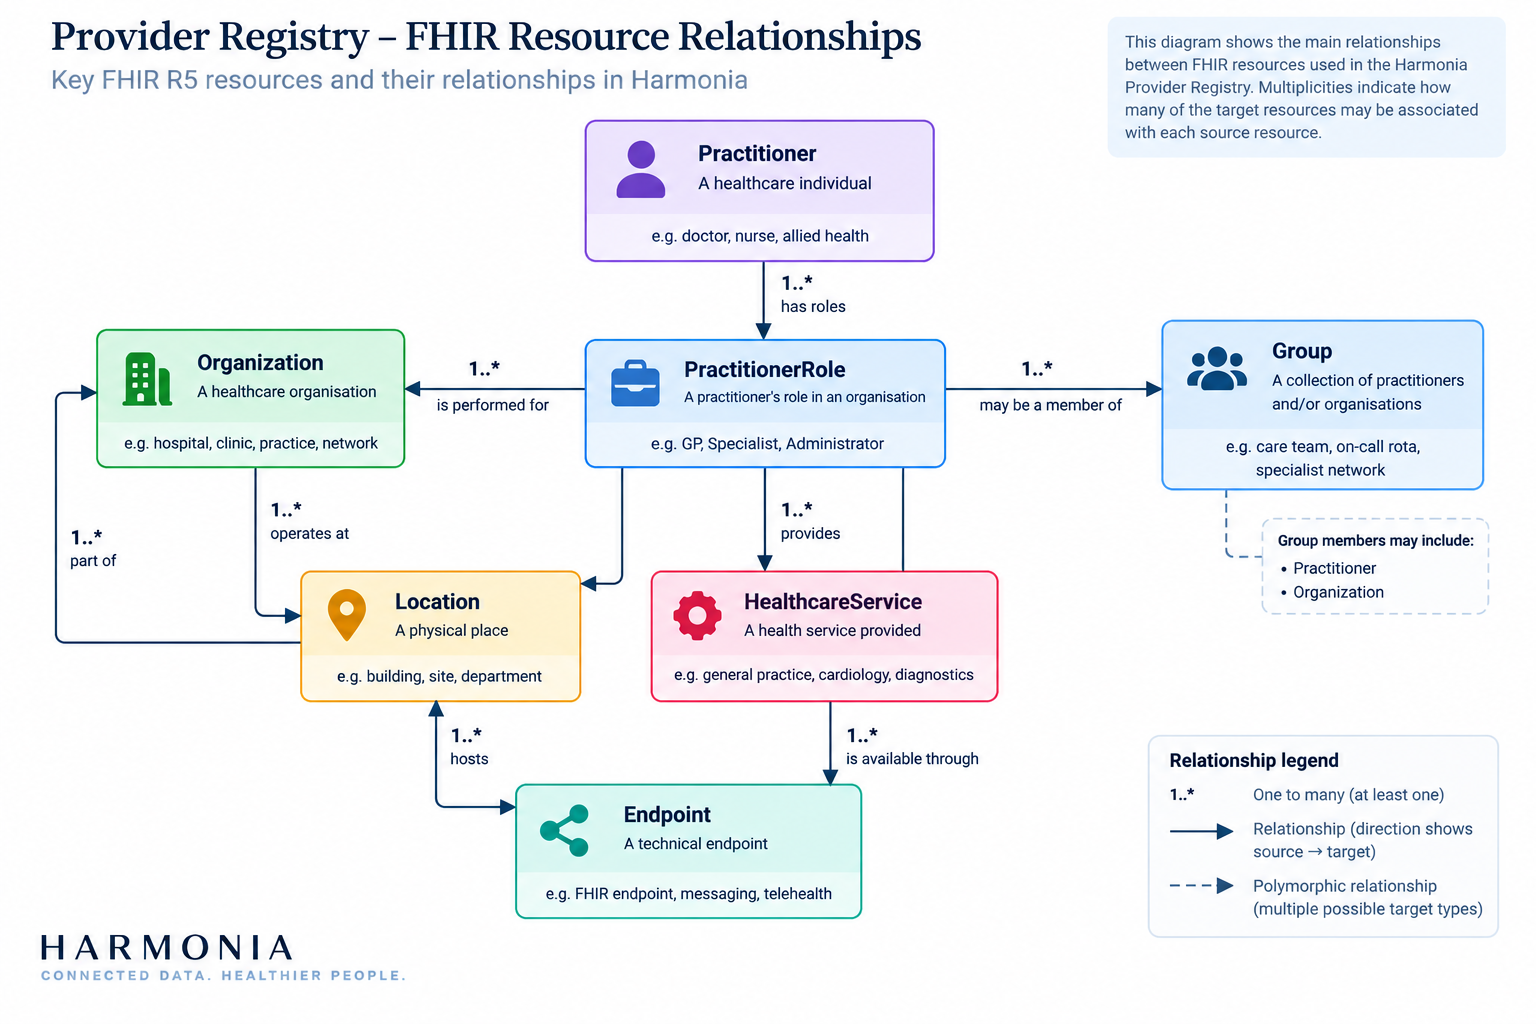
\includegraphics[width=0.94\textwidth, height=0.82\textheight,keepaspectratio]
		{images/fhir-r5-provider-registry-entity-relationship-and-referential-dependency-graph.png}
	}
	\caption{FHIR R5 Provider Registry Entity Relationship and Referential Dependency Graph}
	\label{fig:pr_graph_topology}
\end{figure}

\subsection{Endpoint as an Independent First-Class Entity}
In accordance with architectural standards, \texttt{Endpoint} is modeled and persisted strictly as an independent FHIR resource rather than an embedded string property on PractitionerRole. This allows multiple organizations, facilities, and practitioner roles to share electronic endpoints, support certificate rotation, and manage technical communication parameters (e.g., encryption protocols, payload MIME types, TLS certificates) centrally without duplicating configuration across clinical records.

% =============================================================================
% SECTION E.4: REST API GATEWAY CONTRACT & INTERACTION MATRIX
% =============================================================================
\section{REST API Gateway Contract \& Interaction Matrix}
\label{sec:pr_api_contract}

The \texttt{pylai-fhir-registry} gateway exposes standard FHIR R5 REST endpoints across all seven directory resources plus the \texttt{Task} and \texttt{metadata} operations:

\begin{table}[htbp]
\centering
\small
\begin{tabularx}{\textwidth}{l l p{3.5cm} l X}
\toprule
\textbf{Interaction} & \textbf{Verb} & \textbf{Path / URI} & \textbf{Mode} & \textbf{HTTP Response Codes} \\
\midrule
Read & \texttt{GET} & \texttt{/\{Resource\}/\{id\}} & Synchronous & \texttt{200 OK}, \texttt{404 Not Found}, \texttt{410 Gone} \\
Search & \texttt{GET} & \texttt{/\{Resource\}?\{params\}} & Synchronous & \texttt{200 OK} (\texttt{Bundle}) \\
Create Request & \texttt{POST} & \texttt{/\{Resource\}} & Asynchronous & \texttt{202 Accepted} (\texttt{Location: /Task/\{id\}}), \texttt{400 Bad Request} \\
Update Request & \texttt{PUT} & \texttt{/\{Resource\}/\{id\}} & Asynchronous & \texttt{202 Accepted} (\texttt{Location: /Task/\{id\}}), \texttt{412 Precondition Failed} \\
Task Polling & \texttt{GET} & \texttt{/Task/\{id\}} & Synchronous & \texttt{200 OK} (\texttt{Task}), \texttt{404 Not Found} \\
Metadata & \texttt{GET} & \texttt{/metadata} & Synchronous & \texttt{200 OK} (\texttt{CapabilityStatement}) \\
\bottomrule
\end{tabularx}
\caption{FHIR R5 Provider Registry REST Interaction Matrix}
\label{tab:pr_interaction_matrix}
\end{table}

\subsection{Multi-Parameter Search Capabilities}
The \texttt{FhirStorageService} in Mnemosyne executes multi-parameter search queries supporting standard FHIR search parameters:

\begin{itemize}
    \item \textbf{\texttt{Practitioner}}: \texttt{\_id}, \texttt{identifier} (HPI-I, NPI), \texttt{name} (family, given), \texttt{active}.
    \item \textbf{\texttt{PractitionerRole}}: \texttt{\_id}, \texttt{identifier}, \texttt{practitioner} (reference), \texttt{organization} (reference), \texttt{location} (reference), \texttt{service} (reference), \texttt{active}.
    \item \textbf{\texttt{Organization}}: \texttt{\_id}, \texttt{identifier} (HPI-O), \texttt{name}, \texttt{active}.
    \item \textbf{\texttt{Location}}: \texttt{\_id}, \texttt{identifier}, \texttt{name}, \texttt{organization} (managing organization reference), \texttt{status}.
    \item \textbf{\texttt{HealthcareService}}: \texttt{\_id}, \texttt{identifier}, \texttt{name}, \texttt{organization} (provided-by reference), \texttt{location} (operating site reference), \texttt{active}.
    \item \textbf{\texttt{Endpoint}}: \texttt{\_id}, \texttt{identifier}, \texttt{name}, \texttt{organization} (managing organization reference), \texttt{status}, \texttt{connection-type}.
    \item \textbf{\texttt{Group}}: \texttt{\_id}, \texttt{identifier}, \texttt{name}, \texttt{type}, \texttt{actual} (membership mode: \texttt{true}/\texttt{false}).
\end{itemize}

\subsection{CapabilityStatement Specification (\texttt{GET /metadata})}
The \texttt{CapabilityStatementProvider} dynamically builds an official FHIR R5 \texttt{CapabilityStatement} describing:
\begin{itemize}
    \item FHIR Release \texttt{5.0.0}.
    \item REST server mode with full resource descriptions for all 7 directory types plus \texttt{Task}.
    \item Advertised interactions (\texttt{read}, \texttt{search-type}, \texttt{create}, \texttt{update}).
    \item Exact supported search parameters per resource type.
    \item Security service configuration (\texttt{OAuth2} / \texttt{Bearer} token authentication).
\end{itemize}

\subsection{Asynchronous Task Polling (\texttt{GET /Task/\{id\}})}
When a client polls \texttt{GET /Task/\{id\}}, the \texttt{ProviderRegistryTaskResourceProvider} maps internal \texttt{Pragma} state directly to standard FHIR \texttt{Task} elements:
\begin{itemize}
    \item \texttt{Task.status}: Mapped from \texttt{PragmaStatus} (\texttt{requested} $\rightarrow$ \texttt{in-progress} $\rightarrow$ \texttt{completed} or \texttt{failed}).
    \item \texttt{Task.focus}: References the requested target resource (e.g. \texttt{PractitionerRole/PRR-101}).
    \item \texttt{Task.output}: Upon successful completion, embeds a reference to the persisted resource and resulting version (e.g. \texttt{Practitioner/P-100/\_history/2}). On failure, embeds the diagnostic \texttt{OperationOutcome}.
\end{itemize}

% =============================================================================
% SECTION E.5: GOVERNED CHANGE PROCESSING LIFECYCLE
% =============================================================================
\section{Governed Change Processing Lifecycle \& Pragma State Machine}
\label{sec:pr_lifecycle}

Every asynchronous change request progresses through a deterministic persistent state machine tracked across \texttt{PragmaCheckpoint} records in the \texttt{Mneme} distributed cache and \texttt{Mnemosyne} relational database:

%\begin{lstlisting}[language=bash, caption={Provider Registry Change Request State Progression}]
%+--------------------------------------------------------------------------+
%|                               [ RECEIVED ]                               |
%|               (Gateway validates JSON structure & creates Pragma)        |
%+------------------------------------+-------------------------------------+
%                                     |
%                                     v
%+--------------------------------------------------------------------------+
%|                              [ VALIDATING ]                              |
%|           (Ergon activity executes reference & business checks)          |
%+-------------------+----------------------------------+-------------------+
%                    |                                  |
%           [Validation Failed]                [Validation Passed]
%                    |                                  |
%                    v                                  v
%+---------------------------------------+  +-------------------------------+
%|             [ REJECTED ]              |  |         [ APPROVED ]          |
%|    (Embeds OperationOutcome PR-VAL-*) |  |  (Automatic or Steward Pass)  |
%+---------------------------------------+  +---------------+---------------+
%                                                           |
%                                                           v
%+--------------------------------------------------------------------------+
%|                              [ COMMITTING ]                              |
%|        (Persisting resource to Mnemosyne PostgreSQL & incrementing ver)  |
%+------------------------------------+-------------------------------------+
%                                     |
%                                     v
%+--------------------------------------------------------------------------+
%|                              [ COMPLETED ]                               |
%|        (Resource available for GET/SEARCH; Task status set to completed) |
%+--------------------------------------------------------------------------+
%\end{lstlisting}

\begin{figure}
	\setlength{\fboxrule}{0.5pt}
	\setlength{\fboxsep}{3pt}
    \centering
    \fbox{%
		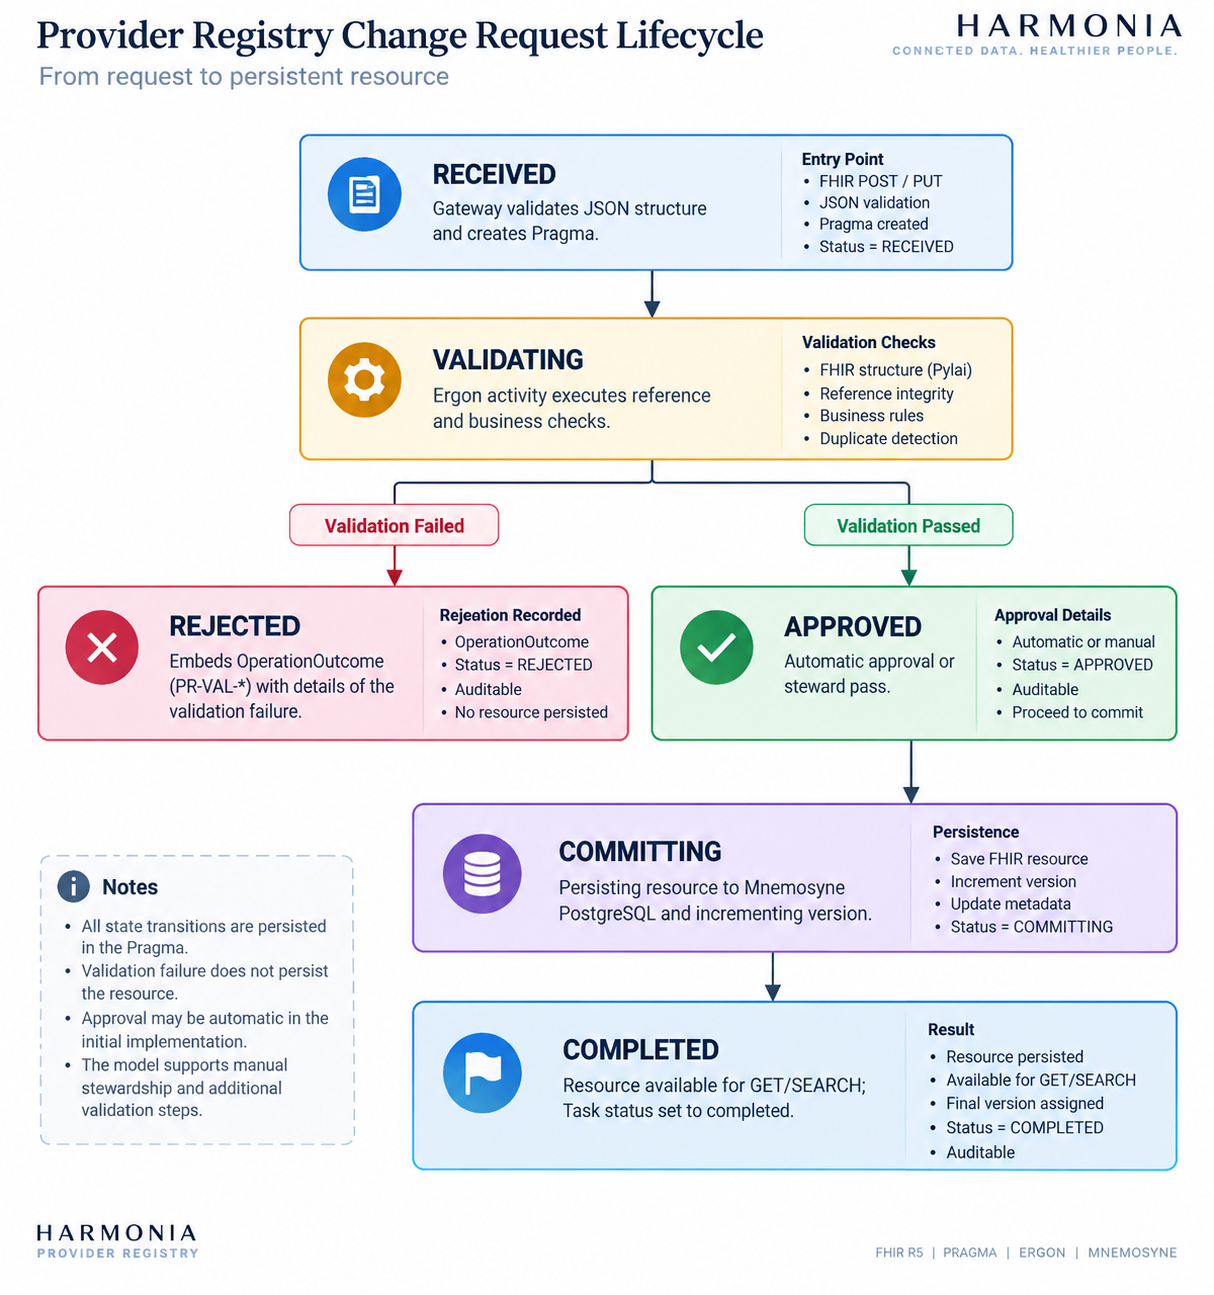
\includegraphics[width=0.94\textwidth, height=0.82\textheight,keepaspectratio]
		{images/provider-registry-change-request-state-progression.png}
	}
	\caption{Provider Registry Change Request State Progression}
	\label{fig:provider-registry-change-lifecycle}
\end{figure}

\subsection{State Machine Transition Rules}
\begin{description}
    \item[\texttt{RECEIVED} $\rightarrow$ \texttt{VALIDATING}]: Triggered when the Ponos WorkEngine consumes the change task from ActiveMQ Artemis and routes to the dedicated resource Ergon activity.
    \item[\texttt{VALIDATING} $\rightarrow$ \texttt{REJECTED}]: Fired when the submitted resource references non-existent or inactive resources, contains duplicate deterministic identifiers, or fails business schema rules. An \texttt{OperationOutcome} is generated and attached to the task output.
    \item[\texttt{VALIDATING} $\rightarrow$ \texttt{APPROVED}]: In the first iteration, change requests that pass all structural, referential, and uniqueness checks are automatically approved. The architecture includes extension hooks for human steward approval workflows.
    \item[\texttt{APPROVED} $\rightarrow$ \texttt{COMMITTING}]: The Ergon persists the approved resource into \texttt{hie\_fhir\_resources}, incrementing the \texttt{version\_id} and stamping \texttt{last\_updated}.
    \item[\texttt{COMMITTING} $\rightarrow$ \texttt{COMPLETED}]: Terminal success milestone. Checkpoints are synchronized, and the task output references the newly persisted resource version.
\end{description}

% =============================================================================
% SECTION E.6: PER-RESOURCE ERGON ACTIVITIES & REFERENTIAL INTEGRITY
% =============================================================================
\section{Per-Resource Ergon Processing Activities \& Referential Integrity Engine}
\label{sec:pr_erga_reference}

Harmonia implements dedicated, strongly-typed Ergon activities extending \texttt{ErgonBase} for each resource type:

\begin{table}[htbp]
\centering
\small
\begin{tabularx}{\textwidth}{l p{4.0cm} X}
\toprule
\textbf{Ergon Activity Class} & \textbf{Target Resource} & \textbf{Specialized Validation \& Verification Responsibilities} \\
\midrule
\texttt{PractitionerChangeErgon} & \texttt{Practitioner} & Validates legal human name, gender, qualifications, and checks duplicate deterministic HPI-I / NPI identifiers in Mnemosyne. \\
\addlinespace
\texttt{PractitionerRoleChangeErgon} & \texttt{PractitionerRole} & Performs deep referential verification ensuring target \texttt{Practitioner}, \texttt{Organization}, \texttt{Location}(s), \texttt{HealthcareService}(s), and \texttt{Endpoint}(s) exist and are active. \\
\addlinespace
\texttt{OrganizationChangeErgon} & \texttt{Organization} & Validates organization name, active status, national identifier (HPI-O), and validates parent organization hierarchy references. \\
\addlinespace
\texttt{LocationChangeErgon} & \texttt{Location} & Validates facility coordinates, addresses, operational status, and verifies managing organization reference existence. \\
\addlinespace
\texttt{HealthcareServiceChangeErgon} & \texttt{HealthcareService} & Validates specialty codes, active status, and verifies provided-by organization and location references. \\
\addlinespace
\texttt{EndpointChangeErgon} & \texttt{Endpoint} & Validates connection type coding, address URL structure, supported payload MIME types, and managing organization reference. \\
\addlinespace
\texttt{GroupChangeErgon} & \texttt{Group} & Validates group membership type (definitional vs actual), member count, and verifies individual member entity references. \\
\bottomrule
\end{tabularx}
\caption{Provider Registry Per-Resource Ergon Activity Responsibilities}
\label{tab:pr_erga_catalog}
\end{table}

\subsection{\texttt{ProviderRegistryReferenceValidator} Engine}
The \texttt{ProviderRegistryReferenceValidator} service in \texttt{mnemosyne-clinical} executes referential integrity inspections against \texttt{hie\_fhir\_resources} before approving changes:
\begin{lstlisting}[language=Java, caption={Reference Validation Contract in ProviderRegistryReferenceValidator}]
public class ProviderRegistryReferenceValidator {
    public ValidationResult validatePractitionerRoleReferences(PractitionerRole role) {
        // 1. Validate mandatory Practitioner reference
        if (role.hasPractitioner()) {
            verifyTargetExistsAndActive("Practitioner", role.getPractitioner().getReference());
        }
        // 2. Validate mandatory Organization reference
        if (role.hasOrganization()) {
            verifyTargetExistsAndActive("Organization", role.getOrganization().getReference());
        }
        // 3. Validate Location references
        for (Reference locRef : role.getLocation()) {
            verifyTargetExistsAndActive("Location", locRef.getReference());
        }
        // 4. Validate HealthcareService references
        for (Reference svcRef : role.getHealthcareService()) {
            verifyTargetExistsAndActive("HealthcareService", svcRef.getReference());
        }
        // 5. Validate Endpoint references
        for (Reference epRef : role.getEndpoint()) {
            verifyTargetExistsAndActive("Endpoint", epRef.getReference());
        }
        return ValidationResult.valid();
    }
}
\end{lstlisting}

If any referenced resource does not exist in Mnemosyne storage or is soft-deleted (\texttt{is\_deleted = true}), the validator returns a structured rejection result with issue code \texttt{PR-VAL-004} (\textit{Reference Not Found}) or \texttt{PR-VAL-005} (\textit{Reference Inactive}), halting the pipeline before mutation.

% =============================================================================
% SECTION E.7: PERSISTENCE, OPTIMISTIC CONCURRENCY & VERSIONING
% =============================================================================
\section{Authoritative Persistence, Optimistic Concurrency \& Versioning Model}
\label{sec:pr_persistence}

Authoritative directory state is persisted in PostgreSQL table \texttt{hie\_fhir\_resources} (detailed in Section~\ref{sec:relational_persistence_schema}).

\subsection{Monotonic Version Incrementing}
When a resource is first created via \texttt{createResource()}, it is assigned:
\begin{equation}
\texttt{version\_id} = 1, \quad \texttt{Meta.versionId} = \text{"1"}, \quad \texttt{Meta.lastUpdated} = \text{now()}
\end{equation}
Subsequent approved updates executed via \texttt{updateResource()} increment the version monotonically ($v_{n+1} = v_n + 1$) and update the \texttt{last\_updated} timestamp atomically.

\subsection{Optimistic Concurrency Control (\texttt{If-Match} / \texttt{ETag})}
To prevent lost updates in concurrent multi-client environments, the Provider Registry supports optimistic concurrency locking:
\begin{enumerate}
    \item When a client reads a resource, the gateway returns the current version in the HTTP header:
    \begin{equation*}
    \texttt{ETag: W/"3"}
    \end{equation*}
    \item When submitting a \texttt{PUT} update, the client supplies the precondition header:
    \begin{equation*}
    \texttt{If-Match: W/"3"}
    \end{equation*}
    \item \texttt{FhirStorageService} checks whether \texttt{entity.getVersionId() == expectedVersion}.
    \item If the database version has advanced (e.g. version 4 exists due to an intervening update), the update is rejected with \texttt{HTTP 412 Precondition Failed} and diagnostic code \texttt{PR-VAL-006}.
\end{enumerate}

% =============================================================================
% SECTION E.8: SECURITY, THEMIS GOVERNANCE & MULTI-TIER AUTHORIZATION
% =============================================================================
\section{Security, Themis Governance \& Multi-Tier Authorization}
\label{sec:pr_security}

The Provider Registry operates under the centralized governance of \textbf{Themis}, enforcing strict separation between identity verification (Authentication at Pylai) and deterministic capability evaluation (Authorization in Themis).

\subsection{Mnemonic Roles and Granular Authority Matrix}
Callers are assigned mnemonic roles (\texttt{HarmoniaRoleEnum}) which Themis policies map to granular authorities (\texttt{HarmoniaAuthorityEnum}):

\begin{table}[htbp]
\centering
\small
\begin{tabularx}{\textwidth}{l l X}
\toprule
\textbf{Role Code} & \textbf{Assigned Authorities} & \textbf{Allowed Operations \& Target Healthcare Actor} \\
\midrule
\texttt{PRV\_RDR} & \texttt{provider.read}, \texttt{provider.search} & Read and search individual directory resources; clinical clients, EMRs. \\
\texttt{PRV\_SUB} & \texttt{provider.change.submit} & Submit asynchronous change requests (\texttt{POST}/\texttt{PUT}); medical registrars. \\
\texttt{PRV\_PROC}& \texttt{provider.change.process}, \texttt{provider.resource.*} & Background Ergon task execution and persistence commit in Ponos. \\
\texttt{PRV\_APR} & \texttt{provider.change.approve}, \texttt{provider.read} & Governance review and clinical change authorization. \\
\texttt{PRV\_ADM} & \texttt{provider.admin}, \texttt{provider.*} & Full directory governance and administrative configuration. \\
\bottomrule
\end{tabularx}
\caption{Provider Registry Mnemonic Role and Granular Authority Matrix}
\label{tab:pr_rbac_matrix}
\end{table}

\subsection{\texttt{FhirSecurityInterceptor} \& Defence-in-Depth Pipeline}
The \texttt{FhirSecurityInterceptor} and downstream processing gates evaluate security deterministically:
\begin{enumerate}
    \item Extracts caller credentials (\texttt{Authorization: Bearer <token>}, \texttt{X-User-Roles}, \texttt{X-Security-Scopes}) and derives \texttt{ThemisPrincipal}.
    \item Invokes \texttt{ThemisService.authorize()} to evaluate default-deny policies (\texttt{ProviderRegistryReadPolicy} for \texttt{GET}, \texttt{ProviderRegistrySubmitPolicy} for \texttt{POST}/\texttt{PUT}).
    \item Attaches immutable caller context to \texttt{ProviderRegistryChangePragma} and serializes claims into FHIR R5 Task extensions.
    \item Ponos dispatch gate and Ergon persistence gates re-verify authorities independently, preventing privilege escalation.
    \item Rejects unauthorized interactions immediately with \texttt{HTTP 403 Forbidden} (\texttt{ForbiddenOperationException}) and logs non-PHI audit records via \texttt{ThemisAuditService}.
\end{enumerate}

% =============================================================================
% SECTION E.9: PARADEIGMA TESTBED & VERIFICATION HARNESS
% =============================================================================
\section{Paradeigma Exemplar Generation \& Verification Testbed}
\label{sec:pr_paradeigma}

To guarantee end-to-end reliability and standard compliance, the \textbf{Paradeigma} simulation framework provides automated synthetic data generators and comprehensive test suites:

\subsection{\texttt{SyntheticProviderRegistryGenerator}}
Generates realistic, fully-interconnected healthcare provider graphs adhering to Australian and international directory standards:
\begin{itemize}
    \item \textbf{Practitioners}: Synthetic physicians, specialists, and nurses with valid Australian HPI-I identifiers (prefix \texttt{800361...}), names, and specialties.
    \item \textbf{Organizations}: Hospital networks, community health clinics, and diagnostic trusts with valid HPI-O identifiers (prefix \texttt{800362...}).
    \item \textbf{Locations}: Acute care wards, outpatient suites, and pathology collection centres with physical addresses.
    \item \textbf{HealthcareServices}: Emergency, Cardiology, Radiology, and General Practice offerings.
    \item \textbf{Endpoints}: Secure FHIR REST, HL7 v2 MLLP, and Secure Messaging electronic endpoints.
    \item \textbf{PractitionerRoles}: Connected relationship graphs linking practitioners to their respective organizations, locations, services, and endpoints.
\end{itemize}

\subsection{Automated Integration \& Verification Test Suites}
The platform includes four dedicated automated test suites in \texttt{paradeigma-test}:
\begin{enumerate}
    \item \textbf{\texttt{ProviderRegistryEndToEndWriteTest}}: Validates the complete asynchronous change lifecycle: submitting \texttt{POST} requests for all 7 resources, receiving \texttt{202 Accepted}, polling \texttt{GET /Task/\{id\}} until \texttt{COMPLETED}, and executing subsequent \texttt{GET} read and search queries to confirm persisted state.
    \item \textbf{\texttt{ProviderRegistryReferentialRejectionTest}}: Submits a \texttt{PractitionerRole} referencing a non-existent \texttt{Practitioner} ID, asserting that the request transitions to \texttt{REJECTED} with error code \texttt{PR-VAL-004} and that no orphan record is persisted.
    \item \textbf{\texttt{ProviderRegistryConcurrencyTest}}: Simulates concurrent updates on the same resource, asserting that stale \texttt{If-Match} preconditions fail with \texttt{PR-VAL-006} concurrency conflict.
    \item \textbf{\texttt{ProviderRegistryRestartRecoveryTest}}: Injects broker restarts during active in-flight change processing, verifying that ActiveMQ Artemis and Ponos resume tasks safely without data loss or duplicate resource generation.
\end{enumerate}

\section{Summary \& Engineering Checklist}
\label{sec:pr_checklist}

Table~\ref{tab:pr_readiness_checklist} summarizes the key engineering invariants and operational checks for the Harmonia FHIR R5 Provider Registry.

\begin{table}[htbp]
\centering
\small
\begin{tabularx}{\textwidth}{l p{4.5cm} X}
\toprule
\textbf{Domain} & \textbf{Architectural Invariant} & \textbf{Verification Criteria} \\
\midrule
\textbf{Gateway} & Governed Write Dichotomy & Ensure \texttt{POST}/\texttt{PUT} returns \texttt{202 Accepted} with \texttt{Location: /Task/\{id\}}; direct synchronous mutation is strictly prohibited. \\
\textbf{Discovery} & Dynamic \texttt{CapabilityStatement} & Validate that \texttt{GET /metadata} accurately reflects all 7 resources, search parameters, and security schemes. \\
\textbf{Validation} & Deep Referential Integrity & Confirm \texttt{ProviderRegistryReferenceValidator} validates all target entity references before approving changes. \\
\textbf{Storage} & Hybrid Relational Document & Verify \texttt{hie\_fhir\_resources} indexes \texttt{resource\_type}, \texttt{fhir\_id}, \texttt{version\_id}, and \texttt{is\_deleted}. \\
\textbf{Concurrency}& Optimistic Locking & Enforce \texttt{If-Match} version validation on all \texttt{PUT} updates. \\
\textbf{Resilience} & Artemis Queue Durability & Verify change requests persist in \texttt{harmonia.provider.registry.change.request} across container restarts. \\
\bottomrule
\end{tabularx}
\caption{Production Readiness Checklist for FHIR R5 Provider Registry Core Services}
\label{tab:pr_readiness_checklist}
\end{table}

\newpage


\end{document}
